\documentclass[dvipsnames, svgnames, x11names, table]{book}
\pdfminorversion=4

\usepackage[linesnumbered,boxruled,algoruled]{myalgorithm2e}
\usepackage{myexercise}
\usepackage{amssymb,latexsym,amsmath,enumerate}     % Standard packages
\usepackage{fancyvrb,url}
\usepackage{verbatim}
\usepackage{hyperref}
\usepackage{array}
\usepackage{graphicx}
\usepackage{float}
\usepackage{tabu}
\usepackage{svg}
\graphicspath{{images/digital-sol/}{images/impl-sol/}}
\newcommand{\simplerisc}{\textit{SimpleRisc }}

\newcommand{\exanswer} {\noindent \textbf{Answer: } }
\newcommand{\proof} {\noindent \textbf{Proof: } }
\newcommand{\mc} {\mathcal}
\newcommand{\header}[1]{ \vskip 4mm \noindent \textbf{#1} \\}
\newcommand{\datalock}{\texttt{Data-Lock }}
\newcommand{\branchlock}{\texttt{Branch-Lock }}
\newcommand{\celsius}{$^\circ$C }
\newcommand{\reg}{\textsl{reg}}
\newcommand{\freg}{\textsl{reg}}
\newcommand{\imm}{\textsl{imm}}
\newcommand{\blabel}{\textsl{label}}
\newcommand{\mem}{\textsl{mem}}
\newcommand{\regp}{\textsuperscript{\textregistered} }
\newcommand{\regtm}{\texttrademark}
\renewenvironment{proof}{Proof: }{\hfill \rule{1ex}{1ex}}

\title{Computer Organisation and Architecture: Solution Manual}
\author{Smruti Ranjan Sarangi}

\begin{document}
\maketitle
\tableofcontents

\chapter{Introduction}
\vskip 1cm
 \begin{flushright}
Solutions by Saumya Sahay $<$saumyasahay98@gmail.com$>$
\end{flushright}
 
\section*{Exercises}
\vskip 1cm
                                                                                     

\section*{Processor and Instruction Set}

\begin{ExerciseList}
\Exercise
Find out the model and make of at least 5 processors in devices around you. The devices can
include desktops, laptops, cell phones, and tablet PCs. 

\Exercise
Make a list of peripheral I/O devices for computers. Keyboards are mice are common devices.
Search for uncommon devices. (HINT: joysticks, game controllers, fax machines)

\Exercise
What are the four properties of an instruction set?

\Exercise
Design an instruction set for a simple processor that needs to perform the following
operations: 
\begin{enumerate}
\item Add two registers
\item Subtract two registers
\end{enumerate}

\Exercise
Design an instruction set for a simple processor that needs to perform the following
operations: 

\begin{enumerate}
\item Add two registers
\item Save a register to memory
\item Load a register from memory
\item Divide a value in a register by two
\end{enumerate}

\Exercise
Design an instruction set
to perform the basic arithmetic operations -- add, subtract, multiply, and divide. 
Assume that all the instructions can have just one operand.

\Exercise[difficulty=1]
Consider the $sbn$ instruction that subtracts the second operand from the first operand,
and branches to the instruction specified by the label (third operand), if the result is negative.
Write a small program using only the $sbn$ instruction to compute the factorial of a positive
number. 
\Answer:
We assume that the variable one is initialised to 1, index to the number whose factorial is to be found and fact to 1.
fact stores the factorial of the number in index at the end of the execution of the program.

\begin{Verbatim}[frame=single]
1:  sbn temp1,temp1
2:  sbn temp1,index
3:  sbn a,temp1
4:  sbn temp,temp
5:  sbn c,c
6:  sbn temp,fact
7:  sbn a,one,11
8:  sbn c,temp
9:  sbn temp2,temp2
10: sbn temp2,one,7 
11: sbn temp2,temp2
12: sbn temp2,c
13: sbn fact,fact
14: sbn fact,c
15: sbn index,one
16: sbn temp, temp
17: sbn temp,index,1
18:<exit>
\end{Verbatim}
\Exercise[difficulty=1]
Write a small program using only the $sbn$ instruction to test if a number is prime. 

\Answer:
We assume that the variable one is initialised to 1, index to the number whose factorial is to be found and b to 1.
The program jumps to label prime if the number is prime and to notprime if the number is not prime.

\begin{Verbatim}[frame=single]
1: sbn a,a
2: sbn temp,temp
3: sbn temp,num
4: sbn a,num,
5: sbn temp1,temp
6: sbn temp1,one
7: sbn b,temp1
8: sbn temp2,temp2
9: sbn temp2,temp
10: sbn temp2,b
11: sbn temp2,one,prime
12: sbn c,c
13: sbn temp4,temp4
14: sbn quo,quo
15: sbn c,one
16: sbn a,b,1
17: sbn quo,c
18: sbn temp4,1,16
19: sbn a,one,not_prime
\end{Verbatim}

\end{ExerciseList}

\section*{Theoretical Aspects of an ISA*}
\begin{ExerciseList}

\Exercise
Explain the design of a modified Turing machine.

\Exercise
Prove that the $sbn$ instruction is Turing complete.

\Exercise
Prove that a machine with memory load, store, branch, and subtract instructions is Turing complete.

\Exercise[difficulty=2]
Find out other models of universal machines from the internet and compare them with
Turing Machines. 
\end{ExerciseList}

\section*{Practical Machine Models}

\begin{ExerciseList}
\Exercise What is the difference between the Harvard architecture and Von Neumann
architecture?

\Exercise What is a register machine? 

\Exercise What is a stack machine? 


\Exercise
Write a program to compute $\mathbf{a + b + c - d}$ on a stack machine. 
\Answer:
\begin{Verbatim}[frame=single]
push d 
push c 
subtract //c-d
push a 
push b 
add    //a+b
add    //a+b+c-d 
pop w
\end{Verbatim}
\Exercise
Write a program to compute $\mathbf{a + b + (c - d)*3}$  on a stack machine. 
\Answer:
\begin{Verbatim}[frame=single]
push d 
push c 
subtract //c-d
push 3
multiply //(c-d)*3
push a 
push b 
add    //a+b
add    //a+b+(c-d)*3
pop w
\end{Verbatim}
\Exercise
Write a program to compute $\mathbf{(a + b/c) *(c - d)+e}$
on a stack machine. 
\Answer:
\begin{Verbatim}[frame=single]
push c
push b
divide // b/c
push a
add    //(a+(b/c))
push d
push c
subtract
multiply   //(a+(b/c))*(c-d)
push e
add    //(a+(b/c))*(c-d)+e
pop w

\end{Verbatim}
\Exercise[difficulty=2]
Try to search the internet, and find answers to the following questions.  
\begin{enumerate}
\item When is having a separate instruction memory more beneficial?
\item When is having a combined instruction and data memory more beneficial?
\end{enumerate}


\end{ExerciseList}





\chapter{Language of Bits}
\section*{Exercises}
\vskip 1cm

\setcounter{Exercise}{0}
\setcounter{Answer}{0}


\section*{Boolean Logic}

\begin{ExerciseList}

\Exercise
$A$, $B$, $C$ and $D$ are Boolean variables. Prove the following results:

\begin{enumerate}[a) ]
\item
$A.B + \overline{A}.B + \overline{B}.C + \overline{B}.\overline{C} = 1$
\item
$(\overline{A} + \overline{B}).(\overline{A}+B).(A + \overline{B}.D+C) = \overline{A}.\overline{B}.D+\overline{A}.C$
\item
$\overline{\overline{A}.\overline{B}+\overline{B}.C} = A.\overline{C} + B$
\item
$A.\overline{B} + \overline{A}.\overline{B} + A.\overline{B}.C.D = \overline{B}$
\end{enumerate}

\Answer:
\begin{enumerate}[a) ]
\item
LHS $= B.(A+\overline{A}) + \overline{B}.(C+\overline{C}) = B + \overline{B} =1$
\item
LHS $= \overline A.(1 + B + \overline B)(A + \overline{B}.D+C) = \overline{A}.\overline{B}.D+\overline{A}.C$
\item
LHS $= (A + B).(B + \overline C) = A.B + B + A.\overline C = B + A.\overline C$
\item
LHS $= \overline B.(A + \overline A) + A.\overline B.C.D = \overline B.(1+A.C.D) = \overline B$

\end{enumerate}

\Exercise 
Construct a circuit to compute the following functions using only NOR gates.
\begin{enumerate}[a)]
\item $overline{A}$
\item $A+B$
\item $A.B$
\item $A \oplus B$
\end{enumerate}

\Exercise 
Construct a circuit to compute the following functions using only NAND gates.
\begin{enumerate}[a)]
\item $overline{A}$
\item $A+B$
\item $A.B$
\item $A \oplus B$
\end{enumerate}

\Exercise[difficulty=2]
Prove that any Boolean function can be realised with just NAND or NOR gates.
[HINT: Use the idea of decomposing a function into its set of minterms.]

\Exercise 
Why are the first and last rows or columns considered to be adjacent in a Karnaugh Map?

\Exercise
Minimise the following Boolean functions using a Karnaugh Map.
\begin{enumerate}[a)]
\item $ABC + AB\overline{C} + \overline{A}BC$
\item $ABCD + A\overline{BC}D + A\overline{D}$
\end{enumerate}

\Exercise[difficulty = 1]
Consider the Karnaugh map of the function $A_1 \oplus A_2 \ldots \oplus A_n$. Prove that
it looks like a chess board. Why cannot we minimise this expression further?

\end{ExerciseList}


\section*{Integer Number Systems}

\begin{ExerciseList}
\Exercise
Convert the following 8 bit binary numbers in 1's complement form to decimal.
\begin{enumerate}[a) ]
\item
01111101
\item
10000000
\item
11111111
\item
00000000
\item
11110101
\end{enumerate}

\Answer:
\begin{enumerate}[a) ]
\item
125
\item
-127
\item
0
\item
0
\item
-10
\end{enumerate}


\Exercise
Convert the following unsigned numbers (in the given base) to decimal:
\begin{enumerate}[a) ]
\item
$(243)_5$
\item
$(77)_8$
\item
$(FFA)_{16}$
\item
$(100)_4$
\item
$(55)_6$
\end{enumerate}

\Answer:
\begin{enumerate}[a) ]
\item
73
\item
63
\item
4090
\item
16
\item
35
\end{enumerate}

\Exercise
Do the following calculations on unsigned binary numbers and write the result as an unsigned binary number.
\begin{enumerate}[a) ]
\item
$1100110101 + 1111001101$
\item
$110110110 + 10111001$
\item
$11101110 - 111000$
\item
$10000000 - 111$
\end{enumerate}
 

\Answer:
\begin{enumerate}[a) ]
\item
11100000010
\item
1001101111
\item
10110110
\item
1111001
\end{enumerate}

\Exercise
What are the pros and cons of the 1's complement number system?

\Exercise
What are the pros and cons of the sign-magnitude number system?

\Exercise
What is a number circle? How is it related to the 2's complement number system? 

\Exercise
What does the point of discontinuity on the number circle signify?

\Exercise 
Why is moving $k$ steps on the number circle in a clockwise direction
equivalent to moving $2^n$ - $k$ steps in an anti-clockwise direction? 
Assume that the number circle contains $2^n$ nodes.

\Exercise
What are the advantages of the 2's complement notation over other number systems?

\Exercise
Outline a method to quickly compute the 2's complement of a number.

\Exercise
Prove the following result in your own words:
    \begin{equation}
		\mc{F}(u - v) \equiv \mathcal{F}(u) + (2^n - \mathcal{F}(v))
	\end{equation}

\Exercise
Let us define {\em sign contraction} to be the reverse of sign extension. What are the rules
for converting a 32 bit number to a 16 bit number by using sign contraction? Can we do this
conversion all the time without losing information?

\Exercise
What are the conditions for detecting an overflow while adding two 2's complement numbers?

\end{ExerciseList}

\section*{Floating Point Number System}
\begin{ExerciseList}
\Exercise
Describe the IEEE 754 format.

\Exercise
Why do we avoid representing the bit to the left of the decimal point in the significand?

\Exercise
Define denormal numbers. How do they help to extend the range of normal floating point numbers?

\Exercise
In the standard form of a denormal number, why is the exponent term equal to $2^{-126}$? Why is
it not equal to $2^{-127}$?

\Exercise
Convert the following floating point numbers into the IEEE 32 bit 754 format. Write your answer in the
hexadecimal format.
\begin{enumerate}[a) ]
\item $-1 * (1.75 * 2^{-29} + 2^{-40} + 2^{-45})$
\item $52$
\end{enumerate}

\Answer :
\begin{enumerate}[a) ]
\item 0xB1601080
\item 0x42500000
\end{enumerate}

\Exercise
What is the range of positive and negative denormalised floating point numbers numbers?
\Answer Range:
\begin{itemize}
\item Positive denormalised numbers: $2^{-149}$ to $(2^{-126} - 2^{-149})$
\item Negative denormalised numbers: $-(2^{-126} - 2^{-149})$ to $-2^{-149}$
\end{itemize}



\Exercise
What will be the output of the following code snippet assuming that the fractions are stored in IEEE 32 bit 754 format:
\begin{Verbatim}[frame=single]
float a=pow(2,-50);
float b=pow(2,-74);
float d=a;
for(i=0; i<100000; i++)
{
	d=d+b;
}
if(d>a) 
	printf("%d",1);
else
	printf("%d",2);
\end{Verbatim}	

\Answer 2

\Exercise
We claim that the IEEE 754 format represents real numbers approximately. Is this statement
correct?

\Exercise[difficulty=1]
Prove that it is not possible to exactly represent $\sqrt{2}$ even if we have an indefinitely
large number of bits in the mantissa.

\Exercise[difficulty=1]
How does having denormal numbers make floating point mathematics slightly more intuitive?

\Exercise[difficulty=1]
What is the correct way for comparing two floating point numbers for equality?


\Exercise[difficulty=2]
Assume that the exponent $e$ is constrained to lie in the range $0 \leq e \leq X$ with a bias of $q$ , and the base is $b$ . The
significand is $p$ digits in length.
Use an IEEE 754 like encoding. However,
you need to devote one digit to store the value to the left of the decimal point in the significand.

\begin{enumerate}[a) ]
\item What are the largest and smallest positive values that can be written in normalised form.
\item What are the largest and smallest positive values that can be written in denormalised form.
\end{enumerate}

\Answer Since the base is b, the most significant digit may not be just 0 or 1, so it will be included in the significand. Therefore, the fraction representation will have 1 digit before decimal, and p-1 digits after decimal point. The valid range of the exponent is 1 to $X-1$. 

\begin{enumerate}[a) ]
\item Largest positive normalised value:
The largest significand is: $(b-1).\underbrace{(b-1) .... (b-1)}_{p-1}$.
This is equal to $(b-1) \times (1 + b^{-1} + \ldots + b^{-(p-1)})$ = $(b - b^{-p+1})$. 
The largest value of the exponent is $X - 1 - q$. Thus the largest normalised value is
\fbox{$(b - b^{-p+1}) \times b^{X - 1 - q}$}. 

Smallest positive normalised value = \fbox{$b^{1-q}$} because the smallest possible
significand is $1.\underbrace{00000}_{p-1}$. 

\item Largest positive denormalised value : 
Largest positive significand with 0 before the decimal point is: $0.\underbrace{(b-1) \ldots (b-1)}_{p-1}$ 
= $(b^{-1} + \ldots b^{-(p-1)}$ = $ (1 - b^{-(p-1)})$. The exponent in a denormalised number: $b^{1-q}$.
Thus, the largest positive denormalised number is \fbox{$(1 - b^{-(p-1)}) \times b^{1-q}$}. 

Smallest positive denormalised value = \fbox{$ b^{1-q} * b^{-(p-1)} = b^{2 - p - q}$}
\end{enumerate}


\Exercise[difficulty=1]
Most of the floating point numbers cannot be represented accurately in hardware due to
 the loss of precision. However, if we choose some other representation, we can 
represent certain kinds of floating point numbers without error.

\begin{enumerate}[a) ]
\item Give a representation for storing rational numbers accurately.
Devise a normalised form for it. 

\item Can other floating point numbers such as $\sqrt{2}$  be represented in a similar way?
\end{enumerate}

\Answer  --

\begin{enumerate}[a) ]
\item
Use 1 bit for the sign (S), and use 16 bits for the numerator, and 16 bits for the denominator. These are 
positive unsigned numbers. 

The normal form is: 
\[
	(-1)^S \times \frac{a}{b} 
\]
Here, $b \ne 0$. $a$ and $b$ are coprime.

\item
We cannot represent $\sqrt{2}$ because it is not a rational number.
\end{enumerate}

\Exercise 
Design a floating point representation, for a base 3 system on the lines of the IEEE 754 format.

\Answer
Each digit can be either 0, 1 or 2. The numbers will have a sign bit $(S)$ which can be 0 or 1.
Let us use 8 digits to represent the exponent ($E$). The bias of the exponent can be $(3^8 - 1)/2$ = 3280.
We need to one digit to represent the digit at the left of the decimal point. We can no longer use
a default value of 1. Thus the mantissa will thus contain (32 - 1 - 8 - 1 = 22) digits.

The normalised form of the  floating point number is:

\[
A = (-1)^S D.M \times 3^{(E - bias)}
\]

bias = 3280, $D \in (1,2)$, $0 \le M < 3$, $1 \le E \le 3^8 - 2$. 

\begin{itemize}
\item
A is 0 if:\\
$D=0$, $M=0$ and $E=0$
\item
A is $+\infty$ if:\\
$S=0$,  $E=3^8-1$ and $M=0$
\item
A is $-\infty$ if:\\
$S=1$,  $E=3^8-1$ and $M=0$
\item
A is NAN if: \\
$E = 3^8 - 1$, and $M \ne 0$
\item
Denormalised form:\\
$D=0$, $M \ne 0$ and $E=0$
\end{itemize}

\end{ExerciseList}
\section*{Strings}

\begin{ExerciseList}
\Exercise
Convert the string ``459801'' to ASCII. The ASCII representation of 0 is 0x30.
Assume that all the numbers are represented in the ASCII format in sequence.

\Answer 
ASCII : 00110100 00110101 00111001 00111000 00110000 00110001

\Exercise
Find the Unicode representation for characters in a non-English language, and compare
it with the ASCII encoding.

\end{ExerciseList}

\section*{Design Problems}
\begin{ExerciseList}
\Exercise
In this section, we have minimised Boolean expressions using Karnaugh maps. We solved
all our examples manually. This method is not scalable for expressions containing
hundreds of variables. Study automated techniques for minimising Boolean expressions
such as the Quinn-McCluskey tabulation method. Write a program to implement this method.

\end{ExerciseList}


\newpage
\chapter{Assembly Language}
\vskip 2cm
\begin{flushright}
Solutions by Saumya Sahay $<$saumyasahay98@gmail.com$>$
\end{flushright}
\section*{Exercises}
\vskip 1cm

\setcounter{Exercise}{0}
\setcounter{Answer}{0}

\section*{Assembly Language Concepts}

\begin{ExerciseList}

\Exercise What is the advantage of the register indirect addressing mode over the memory direct
addressing mode?
\Answer :
\begin{enumerate}
\item The advantages of register indirect addressing mode is that it makes accessing data dynamic rather than static as in the case of direct addressing mode.
ode.
\end{enumerate}

\Exercise 
When is the base-offset addressing mode useful?
\Answer :
Base offset is useful to access fields of a structure or objects.

\Exercise
Consider the base-scaled-offset addressing mode, which directs the hardware to automatically
multiply the offset by 4. When is this addressing mode useful?
\Answer :
Based-scaled offset modeis useful while traversing stacks and complexdata structures.

\Exercise Which addressing modes are preferable in a machine with a large number of registers?
\Answer :
Base index offset, Base index addressing modes,Register indirect addressing.

\Exercise Which addressing modes are preferable in a machine with very few registers?
\Answer :
Immediate addressing,Memory-direct addressing modes.

\Exercise Assume that we are constrained to have at the most two operands per instruction. Design
a format for arithmetic instructions such as add and multiply in this setting.
\Answer :
\begin{enumerate}
\item add R0,R1 (stores the value of R0+R1 in R0)
\item sub R0,R1 (subtracts R1 from R0 and stores in R0)
\end{enumerate}


\end{ExerciseList}

\section*{Assembly Programming}

\begin{ExerciseList}

\Exercise Write simple assembly code snippets in \simplerisc to compute the following: 

\begin{enumerate}[i) ]
\item $a + b + c$
\item $a + b - c/d$
\item $(a + b)*3 - c/d$
\item $a/b - (c*d)/3$
\item $(a\ll2) - (b\gg 3)$ (($\ll$ (left shift logical), $\gg$ (left shift arithmetic))
\end{enumerate}

\Answer :
We store the values of a,b,c and d in registers R0,R1,R2and R3 respectively.\\
\begin{enumerate}
\item \begin{Verbatim}[frame=single]
add R0,R0,R1
add R0,R2,0
\end{Verbatim}
\item \begin{Verbatim}[frame=single]
div R2,R2,R3
add R0,R0,R1
sub R0,R0,R2
\end{Verbatim}
\item \begin{Verbatim}[frame=single]
add R0,R0,R1
mul R0,R0,3
div R2,R2,R3
sub R0,R0,R2
\end{Verbatim}
\item \begin{Verbatim}[frame=single]
div R0,R0,R1
mul R2,R2,R3
div R2,R2,3
sub R0,R0,R2
\end{Verbatim}
\item
\begin{Verbatim}[frame=single]
lsl R0,R0,2
asr R1,R1,3
sub R0,R0,R1
\end{Verbatim}
\end{enumerate}

\Exercise Write a program to load the value $0xFFEDFC00$ into $r0$. Try to minimise
the number of instructions.
\Answer :
\begin{Verbatim}
movh R0,0xFFED
addu R0,R0,0xFC00
\end{Verbatim}

\Exercise
Write an assembly program to set the $5^{th}$ bit 
of register $r0$ to the value of the $3^{rd}$ bit of $r1$. Keep the rest of the contents
of $r0$ the same. The convention
is that the LSB is the first bit, and the MSB 
is the $32^{nd}$ bit. (Use less than or equal to 5 $SimpleRisc$ assembly statements) 
\Answer:
\begin{Verbatim}[frame=single]
and R1,R1,4
lsl R1,R1,2
and R0,R0,0xffef
or R0,R0,R1
\end{Verbatim}

\Exercise
Write a program in \simplerisc assembly to convert an integer stored in memory from the little endian to the big endian format.
\Answer :
\begin{Verbatim}[frame=single]
mov R0,R1
lsl R2,R0,24
lsr R3,R0,24
movu R6,0xff00
movh R7,0x00ff
and R4,R0,R6
lsl R4,R4,8
and R5,R0,R7
lsR R5,R5,8
add R3,R3,R5
add R3,R3,R4
add R2,R2,R3
st R2,[R1]
.print R2
\end{Verbatim}

\Exercise 
Write a program in \simplerisc assembly to compute the factorial of a positive number using an
iterative algorithm.
\Answer:
\begin{Verbatim}[frame=single]
mov R1,1
mov R2,R0
.loop: 
	mul R1,R1,R2
	sub R2,R2,1
	cmp R2,1
	bgt .loop
.exit: .print R1

\end{Verbatim}

\Exercise 
Write a program in \simplerisc assembly to find if a number is prime.
\Answer:
\begin{Verbatim}[frame=single]
mov R2,2
.loop:
	mod R3,R1,R2
	cmp R3,0
	beq .no
	add R2,R2,1
	cmp R2,R1
	bgt .loop
	mov R0,1
	b .exit
.no:
	mov R0,0
.exit:
	.print R0

\end{Verbatim}
\Exercise Write a program in \simplerisc assembly to test if a number is a perfect
square. 
\Answer :
\begin{Verbatim}[frame=single]
mov R2,0
.loop:
	mul R3,R2,R2
	cmp R3,R1
	beq .yes
	add R2,R2,1
	cmp R1,R2
	bgt .loop
	mov R0,0
	b .exit
.yes:
	mov R0,1
.exit:
	.print R0
\end{Verbatim}
\Exercise Given a 32-bit integer in $r3$,
write a \simplerisc assembly program to count the number of 1 to 0 transitions in it. 
\Answer: 
\begin{Verbatim}[frame=single]
movu R1,0x0001
mov R2,32
mov R4,0
mov R5,0
mov R6,R0
.loop1:
	cmp R2,0
	beq .exit
	lsr R6,R0,R5
	and R3,R6,R1
	sub R2,R2,1
	add R5,R5,1
	cmp R3,1
	beq .loop1
.loop2:
	cmp R2,0
	beq .exit
	lsr R6,R0,R5
	and R3,R6,R1
	sub R2,R2,1
	add R5,R5,1
	cmp R3,0
	beq .loop2
	add R4,R4,1
	b .loop1
.exit:
	.print R4
\end{Verbatim}
\Exercise[difficulty=1] 
Write a program in \simplerisc assembly to find the smallest number that is a sum of
two different pairs of cubes. [Note: 1729 is the Hardy-Ramanujan number. $1729 =12^3 + 1^3
= 10^3 + 9^3$].
\Answer :
\begin{Verbatim}[frame=single]

.main:
	mov r0,0
	mov r4,0
	mov r5,0
	mov r6,0
.loop1:
	mov r3,0
	mov r1,1
.loop2:
	mul r4,r1,r1
	mul r4,r4,r1
	cmp r4,r0
	bgt .break2
	mov r2,1
.loop3:
	cmp r2,r1
	bgt .break3
	mul r5,r2,r2
	mul r5,r5,r2
	add r6,r4,r5
	cmp r6,r0
	beq .check
	b .next
.check:
	add r3,r3,1
	cmp r3,2
	beq .break1
.next:
	add r2,r2,1
	b .loop3
.break3:
	add r1,r1,1	
	b .loop2
.break2:
 	add r0,r0,1
   	b .loop1
.break1:
	.print r0

\end{Verbatim}

\Exercise Write a \simplerisc 
assembly program that checks if a 32-bit number is a palindrome.
Assume that the input is available in $r3$. The program should set $r4$
 to 1 if it is a palindrome, otherwise $r4$ should contain a 0.
A palindrome is a number which is the same when read from both
 sides. For example, 1001 is a 4 bit palindrome.
\Answer :
\begin{Verbatim}[frame=single]
	mov R0,1044480
	mov R3,0
	mov R4,31
	movu R2,0x0001
	mov R5,0
	andu R1,R0,0xffff
	.loop:
		and R3,R2,R1
		lsl R2,R2,1
		lsl R3,R3,R4
		add R5,R5,R3
		sub R4,R4,2
		cmp R4,0
		bgt .loop
		lsr R0,R0,16
		lsr R5,R5,16
		sub R0,R5,R0
		cmp R0,0
		beq .palin
		mov R0,0
		b .exit
	.palin:
		mov R0,1
	.exit:
	
\end{Verbatim}
\Exercise Design a \simplerisc program that examines a 32-bit 
value stored in $r1$ and counts the number of contiguous sequences of 1s. For example, the value:
\begin{displaymath}
0111 0001 0001 1110 1100 0111 0001 1111 
\end{displaymath}
contains six sequences of 1s. Write the result in $r2$.
\Answer :
\begin{Verbatim}[frame=single]
movu R1,0x0001
mov R2,32
mov R4,0
mov R5,0
mov R6,R0
.loop1:
	cmp R2,0
	beq .exit
	lsr R6,R0,R5
	and R3,R6,R1
	sub R2,R2,1
	add R5,R5,1
	cmp R3,0
	beq .loop1
	add R4,R4,1
.loop2:
	cmp R2,0
	beq .exit
	lsr R6,R0,R5
	and R3,R6,R1
	sub R2,R2,1
	add R5,R5,1
	cmp R3,1
	beq .loop2
	b .loop1
.exit:
	.print R4

\end{Verbatim}
\Exercise[difficulty=2]
Write a program in \simplerisc assembly to subtract two 64 bit numbers stored
in two registers.

\Exercise[difficulty=2]
In some cases, we can rotate an integer to the right by $n$  positions (less than or equal to 31) so that we obtain the same number.
For example: a 8-bit number 11011011 can be right rotated by 3 or 6
places to obtain the same number.
Write an assembly program
to {\em efficiently} count the number of ways we can rotate a number to the right such that the result is 
equal to the original number. 
\Answer:
\begin{Verbatim}[frame=single]
mov R0,1431655765
mov R1,31
mov R3,R0
.loop:	cmp R1,0
	beq .exit
	lsl R2,R0,31
	lsr R0,R0,1
	sub R1,R1,1
	movu R5,0xffff
	addh R5,R5,0x7fff
	and R0,R5,R0
 	or R0,R0,R2
	cmp R3,R0
 	beq .inc
	 b .loop
.inc :  
	 add R4,R4,1
	 b .loop
.exit : 
	.print R4
\end{Verbatim}
\Exercise[difficulty=2]
A number is known as a cubic Armstrong number if the sum of the cubes of the decimal digits is equal to the
number itself. For example, 153 is a cubic Armstrong number (153 = $1^3 + 5^3 + 3^3$). You are given a number in register, $r0$,
and it is known to be between 1 and 1 million. Can you write a piece of assembly code in $SimpleRisc$ to find out
if this number is an Armstrong number. Save 1 in $r1$ if it is an Armstrong number; otherwise, save 0.
\Answer :
\begin{Verbatim}[frame=single]
mov R4,R1
mov R2,0
.loop:
	mod R2,R1,10
	mul R3,R2,R2
	mul R3,R3,R2
	add R0,R0,R3
	div R1,R1,10
	cmp R1,0
	bgt .loop
	cmp R4,R0
	beq .arms
	mov R5,0
	b .exit
.arms:
	mov R5,1
.exit:
	.print R5
\end{Verbatim}

\Exercise[difficulty=3]
Write a \simplerisc assembly language program to find the greatest common divisor of two binary numbers $u$ and $v$.
Assume the two inputs (positive integers) 
to be available in $r3$ and $r4$. Store the result in $r5$.
[HINT: The gcd of two even numbers $u$ and $v$ is $2*gcd(u/2,v/2)$]
\Answer: 
\begin{Verbatim}[frame=single]
mov R0,42
mov R1,98
mov R4,1
 	cmp R0,0
 	beq .exit
	cmp R1,0 
	beq .case1
.cases:	
	cmp R0,R1
	bgt .exchange
	mod R3,R1,R0
	cmp R3,0
	beq .exit

.case2:
	mod R3,R0,2
	cmp R3,0
	beq .divide1
	b .case3

.divide1:
	div R0,R0,2
	mod R3,R1,2
	cmp R3,0
	beq .check
	b .cases

.check:
	div R1,R1,2
	mul R4,R4,2
	b .cases


.case3:
	mod R3,R1,2
	cmp R3,0
	beq .divide2
	
	sub R0,R1,R0
	div R0,R0,2
	b .cases

.divide2:
	div R1,R1,2
	b .cases

.case1: 
	mov R0,R1
	b .exit

.exchange:
	mov R3,R0
	mov R0,R1
	mov R1,R3
	b .cases
.exit:
	mul R0,R0,R4
\end{Verbatim}

\end{ExerciseList}

\section*{Instruction Set Encoding}

\begin{ExerciseList}

\Exercise Encode the following \simplerisc instructions:

\begin{enumerate}[i) ]
\item $sub$ $sp$, $sp$, 4
\item $mov$ $r4$, $r5$
\item $addu$ $r4$, $r4$, 3
\item $ret$
\item $ld$ $r0$, $[sp]$
\item $st$ $r4$, $8[r9]$
\end{enumerate}
\Answer :
\begin{enumerate}
\item Binary: 00001 1 1110 1110 000000000000000100\\
Hexadecimal : 0x0FB80004  
\item Binary: 01000 0 0100 0000 000000000000000101\\
Hexadecimal:0x41000005
\item Binary: 00000 1 0100 0100 010000000000000011\\
Hexadecimal: 0x05110003
\item Binary: 10100\\
Hexadecimal: 0x00000014
\item Binary:01110 1 0000 1110 000000000000000000\\
Hexadecimal : 0x74380000
\item Binary:01111 1 0100 1001 000000000000001000\\
Hexadecimal : 0x7G240008
\end{enumerate}

\end{ExerciseList}
\section*{Design Problems}
\begin{ExerciseList}
\Exercise

Design an emulator for the \simplerisc ISA. The emulator reads an assembly program line by line, checks each
assembly statement for errors, and executes it. 
Furthermore, define two assembler directives namely $.print$, and $.encode$ to print data on the screen.
The $.print$ directive takes a register or memory location as input. When the emulator encounters the $.print$
directive, it prints the value in the register or memory location to the screen. Similarly, when the emulator
encounters the $.encode$ directive it prints the 32 bit encoding of the instruction on the screen. Additionally,
it needs to also execute the instruction.

\end{ExerciseList}




























\newpage
\chapter{ARM Assembly Language}

\vskip 1cm
\section*{Exercises}
\vskip 1cm

\setcounter{Exercise}{0}
\setcounter{Answer}{0}


\section*{Basic ARM Instructions}

\begin{ExerciseList}

\Exercise
Translate the following code in C to the
ARM instruction set using a minimum number of instructions.
Assume the variables $a$, $b$, $c$, $d$ and $e$ are
32-bit integers and stored in $r0$, $r1$, $r2$, $r3$ and $r4$ respectively. 

\begin{enumerate}
	\item[(a) ] 
\begin{Verbatim}
a=a+b+c+d+e;
\end{Verbatim}
\item[(b) ] 
\begin{Verbatim}
a=b+c;
d=a+b;
\end{Verbatim}
	\item[(c) ]
\begin{Verbatim}
a=b+c+d;
a=a+a;
\end{Verbatim}
	\item[(d) ] 
	\begin{Verbatim}
a=2*a+b+c+d;
\end{Verbatim}
	\item[(e) ] 
\begin{Verbatim}
a=b+c+d; 
a=3*a;
\end{Verbatim}

\end{enumerate}

\Answer:
\begin{enumerate}
	\item[(a) ]
\begin{Verbatim}[frame=single]
add r0, r0, r1
add r0, r0, r2
add r0, r0, r3
add r0, r0, r4
\end{Verbatim}
	\item[(b) ]
\begin{Verbatim}[frame=single]
add r0, r1, r2
add r3, r0, r1
\end{Verbatim}
	\item[(c) ]
\begin{Verbatim}[frame=single]
add r0, r1, r2
add r0, r0, r3
add r0, r0, r0
\end{Verbatim}
	\item[(d) ]
\begin{Verbatim}[frame=single]
add r0, r1, r0, lsl #1
add r0, r0, r2
add r0, r0, r3
\end{Verbatim}
	\item[(e) ]
\begin{Verbatim}[frame=single]
add r0, r1, r2
add r0, r0, r3
add r0, r0, r0, lsl #1
\end{Verbatim}
\end{enumerate} 


\Exercise
Translate the following pieces of code from the 
ARM assembly language to a high level language.
Assume that the variables $a$, $b$, $c$, $d$ and $e$ (containing integers)
are stored in the registers $r0$, $r1$, $r2$, $r3$ and $r4$ respectively.

\begin{enumerate}
\item[(a) ] 
\begin{Verbatim}[frame=single]
add r0, r0, r1
add r0, r0, r2
add r0, r0, r3
\end{Verbatim}
\item[(b) ]
\begin{Verbatim}[frame=single]
orr r0, r0, r1, lsl #1
and r1, r0, r1, lsr #1
\end{Verbatim}
\item[(c) ]
\begin{Verbatim}[frame=single]
add r0, r1, r2
rsb r1, r0, r2
\end{Verbatim}
\item[(d) ]
\begin{Verbatim}[frame=single]
add r0, r1, r2
add r0, r3, r4
add r0, r0, r1
\end{Verbatim}
\item[(e) ]
\begin{Verbatim}[frame=single]
mov r0 #1, lsl #3
mov r0, r0, lsr #1
\end{Verbatim}
\end{enumerate}


\Answer:
\begin{enumerate}
\item[(a) ]
$a=a+b+c+d$;
\item[(b) ]
$a=a\:|\:(b*2)$;\\
$b=a\:\&\:(b/2)$;
\item[(c) ]
$a=b+c$; \\
$b=c-a$;
\item[(d) ]
$a=d+e+b$;
\item[(e) ]
$a=4$;
\end{enumerate}



\Exercise Answer the following:
\begin{enumerate}
\item[(a) ] Write the smallest possible ARM assembly program to load the constant 0xEFFFFFF2 into register
r0.
\item[(*b) ] Write the smallest possible ARM assembly program to load the constant 0xFFFD67FF into register
r0.
\end{enumerate}

\Answer:
\begin{enumerate}
\item[(a) ]
\begin{Verbatim}[frame=single]
mvn r0, #0xD
\end{Verbatim}
\item[(b) ]
\begin{Verbatim}[frame=single]
mvn r0, #0x29800
\end{Verbatim}
\end{enumerate}

\Exercise[difficulty=1]
Using valid ARM assembly instructions, load the constant, 
0xFE0D9FFF, into register r0. Try do to it in the minimum number of instructions. DO NOT use pseudo-instructions or assembler directives.

\Answer 0xFE0D9FFF = $(1111\: 1110\: 0000\: 1101\: 1001\: 1111\: 1111\: 1111)_2$
\begin{Verbatim}[frame=single]
mvn r0, 0x26000
sub r0, r0, 0x1F00000
\end{Verbatim}


\Exercise
Can you give a generic set of ARM instructions or a methodology using which you can load any 32 bit immediate value into a register?
Try to minimise the number of instructions. %Also show that the bound on the number of instructions is tight.

\Answer
Arm architecture allows 12 bits for specifying an immediate with 8 bits of payload and 4 bits to specify rotation. So a 32-bit number can be broken down into 4 sets of 8-bit numbers and then loaded using add instructions.
\\
Example: \\Suppose we want to load the immediate 0xAAAAAAAA into R0. Following are the steps:
\begin{Verbatim}[frame=single]
mov r0, #0xAA
add r0, r0, #0xAA00
add r0, r0, #0xAA0000
add r0, r0, #0xAA000000
\end{Verbatim}



\Exercise
Convert the following C program to ARM assembly. 
Store the integer, $i$, in register $r0$. Assume that the
starting address of array $a$ is saved in register $r1$, and the starting address of array $b$ is saved in register
$r2$.

\begin{Verbatim}[frame=single]
int i;
int b[500];
int a[500];
for(i=0; i < 500; i++) {
    b[i] = a[a[i]];
}
\end{Verbatim}

\Answer:
\begin{Verbatim}[frame=single]
l1:
	ldr r3, [r1, #0]
	add r1, r1, #4
	ldr r4, [r3, #0]
	str r4, [r2, #0]
	add r2, r2, #4
	add r0, r0, #1
	cmp r0, #500
	bne l1
	mov pc, lr
main:
	mov r0, #0
	bl l1
\end{Verbatim}

\Exercise[difficulty=2]
Consider the instruction, {\em mov lr, pc}. Why does this instruction add 8 to the PC, and use that value to set
the value of $lr$? When is this behaviour helpful?
\end{ExerciseList}

\section*{Assembly Language Programming}

\begin{itemize}
\item For all the questions below, assume that two specialised functions, $\_\_div$ and $\_\_mod$, are available.
The $\_\_div$ function divides the contents of $r1$ by the contents of $r2$, and saves the result in $r0$.
Similarly, the $\_\_mod$ function is used to divide $r1$ by $r2$, and save
the remainder in $r0$. Note that in this case both the functions
perform integer division.
\end{itemize}

\vskip 2cm

\begin{ExerciseList}

\Exercise
Write an ARM assembly language program to compute the
2's complement of a number stored in $r0$.
\Answer
Code:
\begin{Verbatim}[frame=single]
rsb r1, r0, #0
\end{Verbatim}



\Exercise
Write an ARM assembly language program that subtracts two 
64-bit integers stored in four registers.

Assumptions:
\begin{itemize}
\item Assume that you are subtracting $A - B$
\item $A$ is stored in register, $r4$ and $r5$. The MSB is in $r4$, and the LSB is in $r5$.
\item $B$ is stored in register, $r6$ and $r7$. The MSB is in $r6$, and the LSB is in $r7$.
\item Place the final result in $r8$(MSB), and $r9$(LSB). 
\end{itemize}

\Answer :
\begin{Verbatim}[frame=single]
sub r9, r5, r7
cmp r5, r7
sub r8, r4, r6
sublo r8, r8, #1
\end{Verbatim}
An alternate smaller code:
\begin{Verbatim}[frame=single]
subs r9, r5, r7
sbc r8, r4, r6
\end{Verbatim}


\Exercise
Write an assembly program to add two 96-bit numbers $A$
 and $B$ using the minimum number of instructions.
$A$ is stored in three registers $r2$, $r3$ and $r4$ 
with the MSB in $r2$ and LSB in $r4$.
$B$ is stored in registers $r5$, $r6$ and $r7$ with the
 MSB in $r5$ and LSB in $r7$. Place the final result in $r8$(MSB), $r9$ and $r10$(LSB).

\Answer :
\begin{Verbatim}[frame=single]
adds r10, r4, r7
adcs r9, r3, r6
adc r8, r2, r5
\end{Verbatim}

\Exercise
Write an ARM assembly instruction code to count the number of 1's in a 32 bit number.

\Answer :
\begin{Verbatim}[frame=single]
l0:
	and r1, r0, r3
	mov r0, r0, lsl #1
	cmp r1, #0
	addne r4, r4, #1
	cmp r0, #0
	bne l0
	mov pc, lr
count:
	mov r4, #0
	mov r0, #1
	bl l0
\end{Verbatim}


\Exercise
Given a 32-bit integer in $r3$,
write an ARM assembly program to count the number of 1 to 0 transitions in it. 

\Answer Code:
\begin{Verbatim}[frame=single]
l1:
	and r1, r3, r0
	mov r0, r0, lsl #1
	and r2, r3, r0
	sub r2, r2, r1, lsl #1
	cmp r2, r0
	addeq r4, r4, #1
	cmp r0, #0x80000000
	bne l1
	mov pc, lr
transition:
	mov r4, #0
	mov r0, #1
	bl l1
\end{Verbatim}


\Exercise[difficulty=1]
Write an ARM assembly program that checks if a 32-bit number is a palindrome.
Assume that the input is available in $r3$. The program should set $r4$
 to 1 if it is a palindrome, otherwise $r4$ should have 0.
A palindrome is a number which is the same when read from both
 sides. For example, 1001 is a 4 bit palindrome.

\Answer Code:
\begin{Verbatim}[frame=single]
l1:
	and r1, r3, r0
	mov r0, r0, lsl #1
	cmp r1, #0
	mov r1, r1, lsl #1
	mov r2, r2, lsl #1
	addne r2, r2, #1
	cmp r0, #0
	bne l1
	mov pc, lr
palin:
	mov r4, #0
	mov r0, #1
	mov r2, #0
	bl l1	
	cmp r3, r2
	moveq r4, #1
\end{Verbatim}


\Exercise
Design an ARM Assembly Language program that will examine a 32-bit 
value stored in $r1$ and count the number of contiguous sequences of 1s. For example, the value:
\begin{displaymath}
0111 0001 0001 1110 1100 0111 0001 1111 
\end{displaymath}
contains six sequences of 1s. Write the final value in register r2. Use conditional instructions
as much as possible.

\Answer Following is the program
\begin{Verbatim}[frame=single]
l0:
	cmp r4, #0
	moveq r4, #1
	addeq r2, r2, #1
	mov pc, lr
l1:
	and r3, r1, r0
	cmp r3, #0
	stmfd sp!, {lr}
	blne l0
	ldmfd sp!, {lr}
	cmp r3, #0
	moveq r4, #0
	mov r0, r0, lsl #1
	cmp r0, #0
	bne l1
	mov pc, lr
count:
	mov r2, #0
	mov r0, #1
	mov r4, #0
	bl l1
\end{Verbatim}


\Exercise[difficulty=2]
In some cases, we can rotate an integer to the right by $n$  positions (less than or equal to 31) so that we obtain the same number.
For example: a 8-bit number 11011011 can be right rotated by 3 or 6
places to obtain the same number.
Write an ARM assembly program
to {\em efficiently} count the number of ways we can rotate a number to the right such that the result is 
equal to the original number. 
\Answer:
\begin{Verbatim}[frame=single]
l0:
	mov r1, #32
	div r4, r1, r0
	mod r2, r1, r0
	cmp r2, #0
	subeq r4, r4, #1
	mov pc, lr
l1:
	cmp r1, r3
	mov r1, r1, ror #1
	add r0, r0, #1
	bne l1
	stmfd sp!, {lr}
	bl l0
	ldmfd sp!, {lr}
	mov pc, lr
count:
	mov r4, #0
	mov r0, #1
	mov r1, r3, ror #1
	bl l1
\end{Verbatim}

\Exercise
Write an ARM assembly program to load and store an integer from memory, where the memory saves it in the
big endian format.

\Answer
Load instruction:
\begin{Verbatim}[frame=single]
ldrb r2, [r0, #0]
mov r1, r2
ldrb r2, [r0, #-1]
add r1, r1, r2, lsl #8
ldrb r2, [r0, #-2]
add r1, r1, r2, lsl #16
ldrb r2, [r0, #-3]
add r1, r1, r2, lsl #24
\end{Verbatim}

Store instruction:
\begin{Verbatim}[frame=single]
and r2, r1, #0xFF
strb r2, [r0, #0]
and r2, r1, #0xFF00
mov r2, r2, lsr #8
strb r2, [r0, #-1]
and r2, r1, #0xFF0000
mov r2, r2, lsr #16
strb r2, [r0, #-2]
and r2, r1, #0xFF000000
mov r2, r2, lsr #24
strb r2, [r0, #-3]
\end{Verbatim}






\Exercise
Write an ARM assembly program to find out if a number is prime using a recursive algorithm.

\Answer:
\begin{Verbatim}[frame=single]
l1:
	mod r5, r3, r4
	cmp r5, #0
	addeq r2, r2, #1
	add r4, r4, #1
	cmp r4, r6
	ble l1
	mov pc, lr
prime:
	mov r7, #0
	mov r3, r0
	mov r6, r0, lsr #1
	mov r4, #1
	mov r2, #0
	bl l1
	cmp r2, #1
	moveq r7, #1
\end{Verbatim}




\Exercise[difficulty=1]
Suppose you decide to take your ARM device to some place with a high amount of radiation,
which can cause some bits to flip, and consequently corrupt data. 
Hence, you decide to store a single bit checksum, which stores the parity of all the other bits, 
at the LSB position of the number (Essentially you can now store only 31 bits of data in a register).
Write an ARM assembly program, which adds the two numbers taking care of the checksum. 
Assume that no bits flip while the program is running. 

\Answer Code
\begin{Verbatim}[frame=single]
l1:
	and r2, r5, r0
	cmp r2, #0
	eorne r1, r1, #1
	mov r0, r0, lsl #1
	cmp r0, #0
	bne l1
	add r5, r5, r1
	mov pc, lr
add:
	mov r0, #2
	mov r1, #0
	mvn r2, #1
	and r3, r3, r2
	and r4, r4, r2
	add r5, r3, r4
	bl l1
\end{Verbatim}





\Exercise[difficulty=1]
Let us encode a 32 bit number by using 2 bits to represent 1 bit. We shall represent logical 0 by 
01, and logical 1 by 10. 
Now let us assume that a 16 bit number 
is encoded and stored in a 32 bit register $r3$. 
Write a program in ARM assembly to convert it back into a 16 bit number, and save the result in $r4$. 
Note that 00 and 11 are invalid inputs and
indicate an error. The program should set $r5$ to 1 in case of an error; otherwise, $r5$ should be 0.

\Answer Program:
\begin{Verbatim}[frame=single]
l1:
	and r1, r3, r0
	mov r4, r4, lsl #1
	cmp r1, r9
	movlo r5, #1
	addeq r4, r4, #1
	cmp r1, r8
	movhi r5, #1
	mov r0, r0, lsr #2
	mov r8, r8, lsr #2
	mov r9, r9, lsr #2
	cmp r0, #0
	bne l1
	mov pc, lr
decode:
	mov r5, #0
	mov r4, #0
	mov r0, #0xC0000000
	mov r8, #0x80000000
	mov r9, #0x40000000
	bl l1
\end{Verbatim}



\Exercise[difficulty=2]
Write an ARM assembly program to convert a 32-bit number to its 12 bit immediate form, 
if possible, with first 4 bits for rotation and next 8 bits for the payload. 
If the conversion is possible, set $r4$ to 1 and store the result in $r5$, 
otherwise, $r4$ should be set to 0. Assume that the input number is available in register $r3$.

\Answer The code:
\begin{Verbatim}[frame=single]
l0:
	and r2, r3, r1
	mov r8, #0
	cmp r2, #0
	movne r8, #1
	cmp r6, #16
	andlt r8, r8, #1
	moveq r4, #0
	moveq pc, lr
	add r6, r6, #1
	cmp r8, #1
	moveq r3, r3, ror #2
	beq l0	
	cmp r2, #0
	movne r4, #0
	addeq r5, r3, r6, lsl #8
	mov pc, lr
immediate:
	mov r4, #1
	mvn r1, #0xFF
	mvn r6, #0
	mov r7, #0
	bl l0
\end{Verbatim}





\Exercise[difficulty=2]
Suppose you are given a 32-bit binary number. You are told that the number has exactly one bit equal to 1;
the rest of the bits are 0. Provide a fast algorithm to find the location of that bit. 
Implement the algorithm in ARM assembly. Assume the input to be available in $r9$. 
Store the result in $r10$.

\Answer
We will use a technique similar to binary search. To check if bit 1 is present to left or right of the middle pivot position, we will start with a filter, which is a sequence of continuous 1's starting from MSB up to the pivot. If bit 1 is left of pivot, new pivot is calculated (as in binary search) and filter is modified using LSL instruction. If bit 1 is right of pivot, new pivot is again calculated and the filter is modified using ASR instruction. Following is the code to implement it.
\begin{Verbatim}[frame=single]
@left = r0
@right = r1
@middle = r2
@filter = r3
l0: 
	@1 to left of middle
	add r1, r2, #1
	add r5, r0, r1
	mov r5, r5, lsr #1
	sub r7, r5, r2
	mov r3, r3, lsl r7
	mov r4, r4, lsl r7
	mov r2, r5
	mov pc, lr
l1:
	@1 to right of middle
	sub r0, r2, #1
	add r5, r0, r1
	mov r5, r5, lsr #1
	sub r7, r2, r5
	mov r3, r3, asr r7
	mov r4, r4, lsr r7
	mov r2, r5
	mov pc, lr
control:
	and r8, r9, r4
	cmp r8, #0
	movne r10, r2
	movne pc, lr
	and r8, r9, r3
	cmp r8, #0
	stmfd sp!, {lr}
	blne l0
	ldmfd sp!, {lr}
	cmp r8, #0
	stmfd sp!, {lr}
	bleq l1
	ldmfd sp!, {lr}
	b control
search:
	mov r0, #31
	mov r1, #0
	mov r2, #15
	mov r3, #0xff000000
	add r3, r3, #0xff0000
	mov r4, #0x10000
	bl control
\end{Verbatim}




\Exercise[difficulty=3]
Write an ARM assembly language program to find the greatest common divisor of two binary numbers $u$ and $v$.
Assume the two inputs (positive integers) 
to be available in $r3$ and $r4$. Store the result in $r5$.
[HINT: The gcd of two even numbers $u$ and $v$ is $2*gcd(u/2,v/2)$]

\Answer
The algorithm, also known as Stein's algorithm is as follows:

\begin{enumerate}
	\item[1. ] $gcd (v, v) = v$
	\item[2. ] $gcd(0, v) = v$, and $gcd(u, 0) = u$ 
	\item[3. ] If $u$ and $v$ are both even, then $gcd(u, v) = 2\:.\:gcd(u/2, v/2)$
	\item[4. ] If $u$ is even and $v$ is odd, then $gcd(u, v) = gcd(u/2, v)$, because $2$ is not a common divisor. Similarly for the other case, then $gcd(u, v) = gcd(u, v/2)$.
	\item[5. ] If $u$ and $v$ are both odd:
	\begin{enumerate}
		\item[i) ] If $u \geq v$, then $gcd(u, v) = gcd((u - v)/2, v)$ 
		\item[ii) ] If $u < v$, then $gcd(u, v) = gcd((v - u)/2, u)$
	\end{enumerate}
\end{enumerate}
Following is the code in ARM assembly language:
\begin{Verbatim}[frame=single]
l0:
	moveq r3, r3, lsr #1
	moveq r4, r4, lsr #1
	add r6, r6, #1
	mov pc, lr
l1:
	cmp r2, #1
	moveq r3, r3, lsr #1
	movne r4, r4, lsr #1
	mov pc, lr
l2:
	cmp r3, r4
	subge r3, r3, r4
	movge r3, r3, lsr #1
	movlt r7, r3
	sublt r3, r4, r3
	movlt r3, r3, lsr #1
	movlt r4, r7
	mov pc, lr
bcase:
	mov r0, #0
	cmp r3, r4
	moveq r5, r3
	addne r0, r0, #1
	cmp r3, #0
	moveq r5, r4
	addne r0, r0, #1
	cmp r4, #0
	moveq r5, r3
	addne r0, r0, #1
	mov pc, lr
case1:
	and r1, r3, #1
	and r2, r4, #1
	add r1, r1, r2
	cmp r1, #0
	stmfd sp!, {lr}
	bleq l0
	ldmfd sp!, {lr}
	cmp r1, #1
	stmfd sp!, {lr}
	bleq l1
	ldmfd sp!, {lr}
	cmp r1, #2
	stmfd sp!, {lr}
	bleq l2
	ldmfd sp!, {lr}
	mov pc, lr
control:
	stmfd sp!, {lr}
	bl bcase
	ldmfd sp!, {lr}
	cmp r0, #3
	moveq r3, r3, lsl r6
	moveq pc, lr
	stmfd sp!, {lr}
	bl case1
	ldmfd sp!, {lr}
	b control
gcd:
	mov r6, #0
	bl control
\end{Verbatim}

\end{ExerciseList}

\subsection*{ARM Instruction Encoding}

\begin{ExerciseList}
\Exercise
How are immediate values encoded in the ARM ISA?

\Exercise
Encode the following ARM instructions. Find the opcodes for 
instructions from the ARM architecture manual~\cite{armbook}.

\begin{enumerate}[i) ]
\item add r3, r1, r2
\item ldr r1, [r0, r2]
\item str r0, [r1, r2, lsl \#2]
\end{enumerate}


\end{ExerciseList}


\subsection*{Design Problems}

\begin{ExerciseList}
\Exercise
Run your ARM programs on an ARM emulator such as the QEMU (\url{www.qemu.org}) emulator, or $arm-elf-run$ (available at \url{www.gnuarm.com}).

\end{ExerciseList}





















\newpage
\chapter{x86 Assembly Language}
\vskip 1cm
\begin{flushright}
Solutions by Saumya Sahay $<$saumyasahay98@gmail.com$>$
\end{flushright}
\section*{Exercises}
\vskip 1cm
\setcounter{Exercise}{0}
\setcounter{Answer}{0}

\section*{x86 Machine Model}


\begin{ExerciseList}

\Exercise
What are the advantages of the segmented addressing mode? Why do modern x86 processors
need the LDT and GDT tables?
 \Answer  :
\begin{enumerate}
\item Protection:Each program can be allocated a certain section of memory .Other programs cannot use this memory, so each program is protected from interference from other programs.
\item Extended memory: Increases the memory a single program can access.
\item Virtualmemory: Expands the address space.
\item Multitasking:Enables the microprocessor to switch from one program to another so the computer can execute several programs at once
\end{enumerate}

The code, data and stack have their own segments in a x86 processor, thus for program execution we need to access the segments related to a process.
The LDT being local to a process, is used to access segments that a process uses as each entry is indexed by segment id, contains starting address of segment, and privileges required to access it.
The GDT  is  a system wide table that is shared by all processes running on machine. For this purpose, it contains pointers to each LDT.\\

\Exercise
Explain the memory addressing modes in x86.
\Answer :
\begin{enumerate}
\item register-indirect: V $\leftarrow$ [r1] . The register saves the address of the memory location that contains the value.
\item base-offset : V $\leftarrow$ [r1+offset] . The base memory address is fetched from r1, constant offset is added and the new memory is accessed by the processor.
\item base-index :V $\leftarrow$ [r1+r2] . The memory address is equal to the sum of register 1 and register 2.
\item base-index-offset :V $\leftarrow$ [r1+r2+offset] . The memory address contains the value as the sum of r1,r2 and offset.
\item base-scaled-index-offset :V $\leftarrow$ [r1+(index*scale) +offset]. The base is in register r1.The index is stored in other register which is multiplied by a power of 2. After this, the offset is added.  
\item memory- direct : V $\leftarrow$ [memory in hexadecimal].
\end{enumerate}

\Exercise
Describe the floating point registers and the floating point stack in x86.
\Answer :
FP registers : A total of 16 registers
\begin{enumerate}
\item 8 general purpose st0 to st7
\item  FPCR Floating-point control register
\item  FPSR Floating-point status register
\item  FPTAG Tag word
\item  FPIOFF Instruction offset
\item  FPISEL Instruction selector
\item  FPDOFF Data offset
\item  FPDSEL Data selector
\end{enumerate}

FP STACK-The FPU has 8 registers---st0 to st7, formed into a stack called FP stack.FPU instructions push numbers onto the stack from memory, are acted upon by fp instructions and then popped off the stack back to memory.\\

\Exercise[difficulty=1]
We can specify an entire 32 bit immediate in a single instruction in x86. Recall that this was not possible in ARM
and \simplerisc. What are the advantages and disadvantages of having this feature in the ISA?
\Answer:
Advantages : 
\begin{enumerate}
\item No memory reference other than instruction fetch is required to obtain the operand, thus saving one memory or cache cycle in the instruction cycle.
\item Specifying an immediate reduces the number of lines of code in a given algorithm.
\end{enumerate}
Disadvantage :
\begin{enumerate}
\item Inflexible: The value retrieved is hard coded and non-changeable, since modification of code once it is running is improper and in many systems impossible.
\end{enumerate} 

\Exercise [difficulty=1]
We claim that using a stack based architecture makes the software very portable. It does not need to be aware of 
the number and semantics of registers in an ISA. Comment on this statement, and try to find other reasons
for preferring a stack based machine.
\Answer:A stack based architecture can get by with just two visible registers, the top of the stack and the next instruction address. It simply works by popping data, performing instructions on it and pushing it back to the stack. The other registers have no immediate need. So, it does not need to be aware of the number and semantics of registers in ISA.

Reasons for preferring a stack based machine is:
\begin{enumerate}
\item Very compact object code: Stack machines have much smaller instructions than the other styles of machines.  
\item Able to use Out-of-Order Execution: Out-of-order execution in stack machines seems to reduce or avoid many theoretical and practical difficulties.
\item Simple compilers: Compilers for stack machines are simpler and quicker to build than compilers for other machines
\item Fast operand access: Since there are no operand fields to decode, stack machines fetch each instruction and its operands at same time. So compared to register machines, stack machines can omit operand fetching stage.
\item Minimal processor state: A machine with an expression stack can get by with just two visible registers, the top-of-stack address and the next-instruction address.
\end{enumerate}

\Exercise[difficulty=2]
Given an arithmetic expression containing floating point operands, how can we evaluate it using a floating point
stack? What should be the order of loading and operating on operands? 
[HINT: A regular arithmetic operation such as -- (1 + 2.5) * 3.9 -- is called an infix expression. To evaluate
expressions using a stack, we need to convert it into a postfix expression of the form -- 1 2.5 + 3.9 *. Here,
we first push 1 and 2.5 on the stack, add the result, push 3.9 on the stack, and multiply the first two entries.
The reader should read more about postfix expressions in textbooks on discrete mathematics.]
\Answer :
We use stack to first convert infix to postfix notation by the stack and then calculate value of postfix expression using a stack.
Transforming Infix to Postfix :
Let Q be the arithmetic expression in infix notation and  P be the equivalent postfix expression.
\begin{enumerate}
\item Push left paranthesis onto Stack and add right parenthesis to the end of Q.
\item Scan Q from left to right and repeat steps 3 to 6 for each element of Q until STACK is empty
\item If an operand is encountered add it to P
\item If a left parenthesis is encountered, push onto STACK
\item If an operator op is encountered , then:
     Repeatedly pop from STACK and add to P each operator on the top of STACK which has the same precedence as or higher precedence than op\\
     Add op to STACK\\
---End of If structure
\item If a right parenthesis is encountered, then:
Repeatedly pop from STACK and add to P each operator until a left parenthesis is encountered.\\
Remove the left parenthesis.\\
---End of If structure
---End of Step 2 loop
\item Exit
\end{enumerate}
Evaluation of postfix :
\begin {enumerate}
\item Add a right parenthesis at the end of P
\item Scan P from left to right and repeat steps 3 and 4 for each element of P until parenthesis is encountered.
\item If an operand is encountered , put it on STACK .
\item If an operator op is encountered
               Remove the top two elements of STACK, A being the top element and B being the other one.\\
               Evaluate B op A.\\
               Place the result of this evaluation back on STACK.\\
---End of If structure
---End of Step 2 loop
\item Pop the top element of STACK to get the final value of the mathematical expression.
\item Exit\\
\end{enumerate}


\end{ExerciseList}
\section*{Assembly Programming using Integer Instructions}

\begin{ExerciseList}
\Exercise Write x86 assembly code snippets  to compute the following: 

\begin{enumerate}[i) ]
\item $a + b + c$
\item $a + b - c/d$
\item $(a + b)*3 - c/d$
\item $a/b - (c*d)/3$
\item $(a\ll2) - (b\gg 3)$ (($\ll$ (left shift logical), $\gg$ (left shift arithmetic))
\end{enumerate}
\Answer :

\begin{enumerate}
\item \begin{Verbatim}[frame=single]
mov eax,[a]
add eax,[b]
add eax,[c]
\end{Verbatim}
\item 
\begin{Verbatim}[frame=single]
mov eax,[c]
mov ebx,[d]
idiv ebx
mov ebx,[a]
mov ecx,[b]
add ebx,ecx
sub ebx,eax
\end{Verbatim}
\item
\begin{Verbatim}[frame=single]
mov eax,[a]
mov ebx,[b]
imul ecx,[eax+ebx],3
mov eax,[c]
mov ebx,[d]
idiv ebx
sub ecx,eax
\end{Verbatim}
\item 
\begin{Verbatim}[frame=single]
mov eax,[c]
mov ebx,[d]
imul ebx,eax
mov eax,3
idiv ebx
mov ebx,eax
mov eax,[a]
mov ecx,[b]
idiv ecx
sub eax,ebx
\end{Verbatim}
\item \begin{Verbatim}[frame=single]
mov eax,[a]
shl eax,2
mov ebx,[b]
shr eax,3
sub eax,ebx
\end{Verbatim}
\end{enumerate}
\Exercise
Write an assembly program to convert an integer stored in memory from the little endian to the big endian format.
\Answer:
\begin{Verbatim}[frame=single]
mov eax,[num]
mov ebx,eax
shr ebx,24
mov ecx,0
or ecx,ebx
mov ebx,eax
and ebx,0x000000ff
shl ebx,24
or ecx,ebx
mov ebx,eax
and ebx,0x00ff0000
shr ebx,8
or ecx,ebx
mov ebx,eax
and ebx,0x0000ff00
shl ebx,8
or ecx,ebx
\end{Verbatim}
\Exercise 
Compute the factorial of a positive number using an
iterative algorithm.
\Answer  :
\begin{Verbatim}[frame=single]
	mov eax,[num]
	mov ebx, 2
	mov ecx, 1
.fact:
       imul ecx,ebx
       inc ebx
       cmp ebx,eax
       jle.fact
exit:
\end{Verbatim}
\Exercise 
Compute the factorial of a positive number using a
recursive algorithm.
\Answer  :
\begin{Verbatim}[frame=single]
		mov eax,[num]
function:
               mov ebx, 1
               cmp, eax, 1
               je.return
               push eax
               dec eax
               call function
               pop eax
               imul ebx,eax
.return:
               ret
\end{Verbatim}
\Exercise 
Write an assembly program to find if a number is prime.
\Answer  :
\begin{Verbatim}[frame=single]
	mov eax,[num]
	mov ebx, 2
	mov ecx , eax
.prime:
           mov edx, 0 
           idiv ebx
           cmp edx, 0
           je.notprime
           inc ebx
           mov eax, ecx
           cmp ebx, eax
           jl.prime
           mov eax, 1
           jmp.exit
.notprime:
           mov eax 0
.exit:
\end{Verbatim}

\Exercise Write an assembly program to test if a number is a perfect
square. 
\Answer :
\begin{Verbatim}[frame=single]
	mov eax,[num]
	mov ebx, 0
	mov ecx, 1
.square:
        mov edx,ecx
        imul edx,ecx
        cmp edx,eax
        je .perfect
        inc ecx
        cmp ecx,eax
        jne .square
        mov ebx,0
.perfect:
        mov ebx, 1
.exit:
\end{Verbatim}

\Exercise Write an assembly program to test if a number is a perfect
cube.
\Answer :
\begin{Verbatim}[frame=single]
	mov eax,[num]
	mov ebx, 0
	mov ecx, 1
.cube:
        mov edx,ecx
        imul edx,ecx
	imul edx,ecx
        cmp edx,eax
        je .perfect
        inc ecx
        cmp ecx,eax
        jne .cube
        mov ebx,0
.perfect:
        mov ebx, 1
.exit:
\end{Verbatim}
\Exercise Given a 32-bit integer, count the number of 1 to 0 transitions in it. 
\Answer :
\begin{Verbatim}[frame=single]
main:    
       mov eax, [num]   
       mov ecx,32   
       mov ebx,0   
.loop: shr eax, 1
        jc .loop
.loop2: jz .exit
        shr eax, 1
        jnc .loop2
        inc ebx
        jmp .loop
.exit:  
\end{Verbatim}
\Exercise Write an assembly program that checks if a 32-bit number is a palindrome.
A palindrome is a number which is the same when read from both sides. For example, 1001 is a 4 bit palindrome.
\Answer :
\begin{Verbatim}[frame=single]
mov eax,[num]
mov ebx,0x00000001
mov ecx,0x80000000
mov edx,31
.loop:  test eax,ecx
	jnz .one

.zero:  test eax,ebx
	jz .next
	jmp .no

.next:  sub edx,1
	cmp edx,0
	je .yes
	shr ecx,1 
	shl ebx,1
	jmp .loop

.yes:   mov ecx,1
	jmp .exit

.one:   test eax,ebx
	jnz .next

.no:    mov ecx,0
.exit:
\end{Verbatim}
\Exercise Write an assembly program to examine a 32-bit 
value stored in $eax$ and count the number of contiguous sequences of 1s. For example, the value:
\begin{displaymath}
0111 0001 0001 1110 1100 0111 0001 1111 
\end{displaymath}
contains six sequences of 1s. Write the final value in register r2.
\Answer :
\begin{Verbatim}[frame=single]
 mov eax, [num]
 mov ecx,32
 mov ebx,0 
.loop1:
	dec ecx
	cmp ecx,0 
	jl .exit
	shr eax,1 
	jc .loop2
	jmp .loop1
.loop2: 
	shr eax, 1
	dec ecx
	jc .loop2
	inc ebx
	jmp .loop1
.exit:
\end{Verbatim}
\Exercise
Write an assembly program to count the number of 1's in a 32 bit number.
\Answer :
\begin{Verbatim}[frame=single]
    mov eax, [num]
    mov ecx,32
    mov edx,0 
.loop:dec ecx
      cmp ecx,0
      jl .exit
      shl eax,1
      jnc .loop
      inc edx
      jmp .loop
.exit:
 
\end{Verbatim}
\Exercise[difficulty=1] 
Write an assembly program to find the smallest number that is a sum of
two different pairs of cubes. [Note: 1729 is known as the Hardy-Ramanujan number. $1729 =12^3 + 1^3
= 10^3 + 9^3$]. 

\Exercise[difficulty=2]
In some cases, we can rotate an integer to the right by $n$  positions (less than or equal to 31) so that we obtain the same number.
For example: a 8-bit number 11011011 can be right rotated by 3 or 6
places to obtain the same number.
Write an assembly program
to {\em efficiently} count the number of ways we can rotate a number to the right such that the result is 
equal to the original number. 
\Answer :
\begin{Verbatim}[frame=single]
mov eax, [num]    
    mov ecx,32  
    mov ebx,0  
    mov edx,eax  
.loop:  
    dec ecx  
    cmp ecx,1  
    jl .exit  
    ror eax,1  
    cmp edx,eax  
    jne .loop  
    inc ebx  
    jmp .loop  
.exit:  
\end{Verbatim}
\Exercise[difficulty=3]
Write an assembly language program to find the greatest common divisor of two binary numbers $u$ and $v$.
Assume the two inputs (positive integers) 
to be available in $eax$ and $ebx$. Store the result in $ecx$.
[HINT: The gcd of two even numbers $u$ and $v$ is $2*gcd(u/2,v/2)$]
\Answer :
\begin{Verbatim}[frame=single]
mov eax,[num1]
mov ebx,[num2]
mov ecx,1
.cases: cmp eax,0 ;num2=0
	je .exit
	cmp ebx,0 ;num1=0 
 	je .case1	
	cmp eax,ebx ;num1=num2
	je .exit

.case2: mov edx,eax  ;num1 is even
	test edx,1
	jnz .case3

.check: sar eax,1
	mov edx,ebx  ;both even
	test edx,1
	jz .mul
	jmp .cases

.case3: mov edx,ebx  ;only num2 is even 
	test edx,1
	jnz .case4
	sar ebx,1
	jmp .cases
	
.case4: mov edx,eax  ;both odd
	and eax, ebx
	test eax, 1
	jz .cases
	mov eax,edx
	cmp eax,ebx
	jl .exchange
	sub eax,ebx
	sar eax,1
	jmp .cases
	
.mul:   sar ebx,1  ;counter for 2*gcd(even/2,even/2)
	sal ecx,1
	jmp .cases

.case1: xchg eax,ebx
	jmp .exit

.exchange: xchg eax,ebx
	   jmp .case4
.exit:     imul ecx,ebx
\end{Verbatim}
\Exercise
Write an assembly program that uses string instructions to set the value of a range of memory addresses to 0.
Reduce the code size by using the $rep$ prefix.
\Answer :
\begin{Verbatim}[frame=single]
cld  
mov eax 0  
mov ecx 10  
rep stosd
\end{Verbatim}

\end{ExerciseList}


\section*{Assembly Programming using Floating Point Instructions}

\begin{ExerciseList}
\Exercise
Why is the $mov$ instruction a very versatile instruction?
\Answer
The mov instruction in x86 is able to move the contents of a register, immediate or even memory location into another memory location or register(Exception:Source and Destination can't both be memory locations).This way the mov instruction can achieve the function of loading and storing memory values because it accepts memory operands, preventing us from dedicating any seperate load/store instruction in x86 and allowing us to fuse the functionality of three RISC instructions into a single CISC instruction.

\Exercise
Write an assembly program to find the roots of the equation $x^2 - x - 1 = 0$. Recall that the roots
of a quadratic equation of the form $ax^2 + bx+ c$ are equal to $\frac{-b \pm \sqrt{b^2 - 4ac}}{2a}$.
\Answer :
\begin{Verbatim}[frame=single]
fld dword [b]
fmul st0
fstp dword [esp]
fld dword [a]
fld dword [c]
fmul st1
fadd st0
fadd st0
fld dword [esp]
fsub st0,st1
comi st0,0
jl .no_real
fsqrt st0
fld dword [b]
fneg st0
fld dword [esp]
fadd st0,st1
fstp dword [esp]
fld dword [a]
fadd st0
fld dword [esp]
fdiv st1
\end{Verbatim}

\Exercise Verify the following trigonometric identities for random values of $\theta$ using assembly
programs. Use the
$rdrand$ instruction that loads a random 32 bit integer into a register.

\vskip 1cm

\begin{center}
\begin{tabular}{||l|l||}
\hline
\hline
S. No. & Identity \\
\hline
1 & $sin^2(\theta) + cos^2(\theta) = 1$ \\
\hline
2 & $sin \left ( \frac{\pi}{2} - \theta \right ) = cos(\theta)$ \\
\hline
3 & $cos(\theta + \phi) = cos(\theta)cos(\phi) - sin(\theta)sin(\phi)$ \\
\hline
4 & $sin(\theta) + sin(\phi) = 2 sin \left ( \frac{\theta + \phi}{2} \right ) cos \left ( \frac{\theta - \phi}{2} \right
)$  \\
\hline
\hline
\end{tabular}
\end{center}
\Answer :
\begin{enumerate}
\item \begin{Verbatim}[frame=single]
	fld dword [theta]
	fsin
	fmul st0
	fstp dword [esp]
	fld dword [theta]
	fcos
	fmul st0
	fld dword [esp] 
	fadd st0,st1
	fld dword [one]
	fsub st0,st1
	fabs
	fld dword [threshold]
	fsub st0,st1
	ja .equal
	mov eax, 0
	jmp .exit

.equal:
	mov eax, 1
.exit:
\end{Verbatim}
\item \begin{Verbatim}[frame=single]

	fld dword [theta]
	fld dword [pi]
	fdiv dword [two]
	fsub st0,st1
	fsin
	fstp dword [esp]
	fld dword [theta]
	fcos
	fld dword [esp] 
	fsub st0, st1
	fld dword[threshold]
	comi st0,st1
	ja.equal
	mov eax, 0
	jmp .exit

.equal:
	mov eax, 1
.exit:
\end{Verbatim}

\item \begin{Verbatim}[frame=single]

	fld dword [theta] 
	fcos
	fld dword [fi]
	fcos
	fmul st0,st1
	fstp dword [esp]
	fld dword [theta]
	fsin
	fld dword [fi]
	fsin
	fmul st0,st1
	fld dword [esp]
	fsub st0,st1
	fstp dword [esp] 
	fld dword [theta]
	fld dword [fi]
	fadd st0,st1
	fcos
	fld dword [esp]  
	fsub st0, st1
	fld dword [threshold]
	fcomi st0, st1
	ja .equal
	mov eax, 0
	jmp .exit

.equal:
	mov eax, 1
.exit:
\end{Verbatim}

\item \begin{Verbatim}[frame=single]
	fld dword [theta]
	fsin
	fld dword [fi]
	fsin
	fadd st0,st1
	fstp dword [esp]
	fld dword [theta]
	fld dword [fi]
	fadd st0,st1
	fdiv dword [two]
	fsin
	fadd st0
	fld dword [theta]
	fld dword [fi]
	fsub st0,st1
	fcos
	fmul st0,st2
	fld dword [esp]  
	fsub st0, st1
	fld dword [threshold]
	fcomi st0, st1
	ja .equal
	mov eax, 0
	jmp .exit

.equal:
	mov eax, 1
.exit:

\end{Verbatim}
\end{enumerate}
\Exercise
Assume that we have two arrays of 10 floating point numbers, where the starting addresses of the arrays are stored in
$eax$ and $ebx$ respectively. Find the arithmetic mean (AM), geometric mean (GM), and harmonic mean (HM) using 
assembly routines. Verify that $AM \ge GM \ge HM$. 

\Exercise[difficulty=1]
Let us compute the value of the constant, $e$ using an assembly program.
Use the following mathematical expression.
\[
	e = 1 + \frac{1}{1!} + \frac{1}{2!} + \frac{1}{3!} + \frac{1}{4!} + \ldots + \frac{1}{10!}
\]

\Exercise[difficulty=2]
For random values of $\theta$ show that following identity holds:
\[
sin(\theta) = \theta - \frac{\theta^3}{3!} + \frac{\theta^5}{5!} - \ldots
\]

\end{ExerciseList}

\section*{x86 ISA Encoding}

\begin{ExerciseList}
\Exercise
What are the values of the SIB and ModR/M bytes for the instruction, {\em mov eax, [eax + ebx*4]}?
\Answer :
ModR/M :0x08 \\
SIB    :0x98\\
\Exercise
What are the values of the SIB, ModR/M, and displacement bytes for the instruction, {\em mov eax, [eax + ebx*4 + 32]}?
\Answer :
ModR/M :0x44\\
SIB    :0x0x98\\
Displacement bytes:0x20\\   
\Exercise
What is the value of the $ModR/M$ byte when we need to specify a memory address that does not have any base
or index registers? Assume that the value of the $reg$ field is 000. 
\Answer:
ModR/M: 0x03

\Exercise[difficulty=1] Assume that we have an instruction that has a single operand of the form $[ebp]$. How do we encode it
using the fields in the ModR/M byte?
\Answer:
ModR/X :0x48

\Exercise[difficulty=1] What are the values of the SIB and ModR/M bytes for the instruction, {\em mov eax, [ebx*4]}?
\Answer:
ModR/M:0x04\\
SIB   :0x9D  

\end{ExerciseList}


\subsection*{Design Problems}

\begin{ExerciseList}
\Exercise
Write an x86 assembly emulator that can read an assembly file, and execute each assembly instruction one by one.

\Exercise
Use the GNU compiler to generate an assembly file for a test program written in C using the command, {\em gcc -S
-masm=intel}. 

\end{ExerciseList}































\newpage
\chapter{Logic Gates, Registers, and Memories}
\begin{flushright}
\textbf{Solutions prepared by Prajwala TM $<$prajwala.tm@gmail.com$>$}
\end{flushright}
\section*{Exercises}
\vskip 1cm

\setcounter{Exercise}{0}
\setcounter{Answer}{0}


\section*{Transistors and Logic Gates}

\begin{ExerciseList}
\Exercise
Describe the operation of a P-N junction.
\Answer
The majority carriers on the $n$ side are electrons whereas those on the $p$ side are holes. When a junction is formed in a silicon wafer by doping, a concentration gradient is created between $p$-type and $n$-type materials. This results in electrons moving from $n$ side to 
$p$ side and holes moving from $p$ side to $n$ side through the junction. When an electron leaves the $n$-side region, it leaves behind an ionised donor (a positive charge). Similarly when a hole is diffused to $n$-side, it leaves behind an ionised acceptor (a negative charge).  This movement of electrons from $n$-side to $p$-side (n$\rightarrow$p) and the movement of holes from $p$-side to $n$-side is called (p$\rightarrow$n) “diffusion” and it results in a current named as “diffusion current“.When more and more electrons leaves the $n$-region and more and more holes leaves the $p$-region, a region of positive and negative charges is formed at the junction. Positive charges get accumulated near the $n$-side junction and negative charges get accumulated near the $p$-side junction. This region is known as “depletion” region.Thus, there is a layer of -ve charges accumulated at the $p$-side of junction and a layer of +ve charges accumulated at the $n$-side of the junction. This results in the formation of an electric field directed from positive charge to negative charge. This electric field causes electrons to move from $p$ side to $n$ side (p$\rightarrow$n) and the holes to move from $n$ side to $p$ side 
(n$\rightarrow$p). This motion of charge carriers due to electric field is known as “drift”.The current resulting from the flow of electrons and holes due to this electric field (generated by depletion region) is known as “drift current”.
At steady state, the drift and diffusion currents balance each other , and there is effectively "NO CURRENT FLOW" across the junction.
\Exercise
Define drift and diffusion current.
\Answer
Diffusion current is the current in a p-n junction caused by the diffusion of charge carriers (holes and/or electrons) due to the concentration gradient between the n and p sides of the p-n junction. The drift current is the current due to the motion of charge carriers caused by the force exerted on them by an electric field across the depletion region.
\Exercise
Describe the operation of a NMOS transistor? 
\Answer
An NMOS transistor is made by connecting two p-n junctions. It consists of a central substrate of $p$-type doped silicon. There are two small regions on both sides containing $n$-type doped silicon. These are known as $source$ and $drain$ respectively. The region in the middle of the source and drain is known as $channel$. On top of the channel, there is a thin insulating layer typically made of silicon dioxide, and is covered by a metallic or polysilicon based conducting layer. This is called the $gate$.\\
Each of these terminals - source, drain, gate can be connected to a voltage source. The gate voltage can be either logical 1 or logical 0. If the gate voltage is logical 1, then the electrons in the channel get attracted towards the gate. If the voltage at the gate is larger than a certain voltage known as "Threshold voltage", then a low resistance conducting path is formed between the drain and source due to accumulation of electrons. Thus, a current can flow between the drain and source. Hence, when the gate voltage is a logical 1, the NMOS transistor switch is turned on. If its a logical 0, then the switch is turned off. 
\begin{figure}[H]
  \centering
  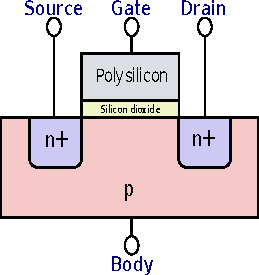
\includegraphics[width=10cm,height=5cm,clip=true,keepaspectratio]{nmos.pdf}
\end{figure}
\Exercise
Draw the circuit of a CMOS inverter, NOR gate, and NAND gate.
\begin{figure}[H]
  \centering
  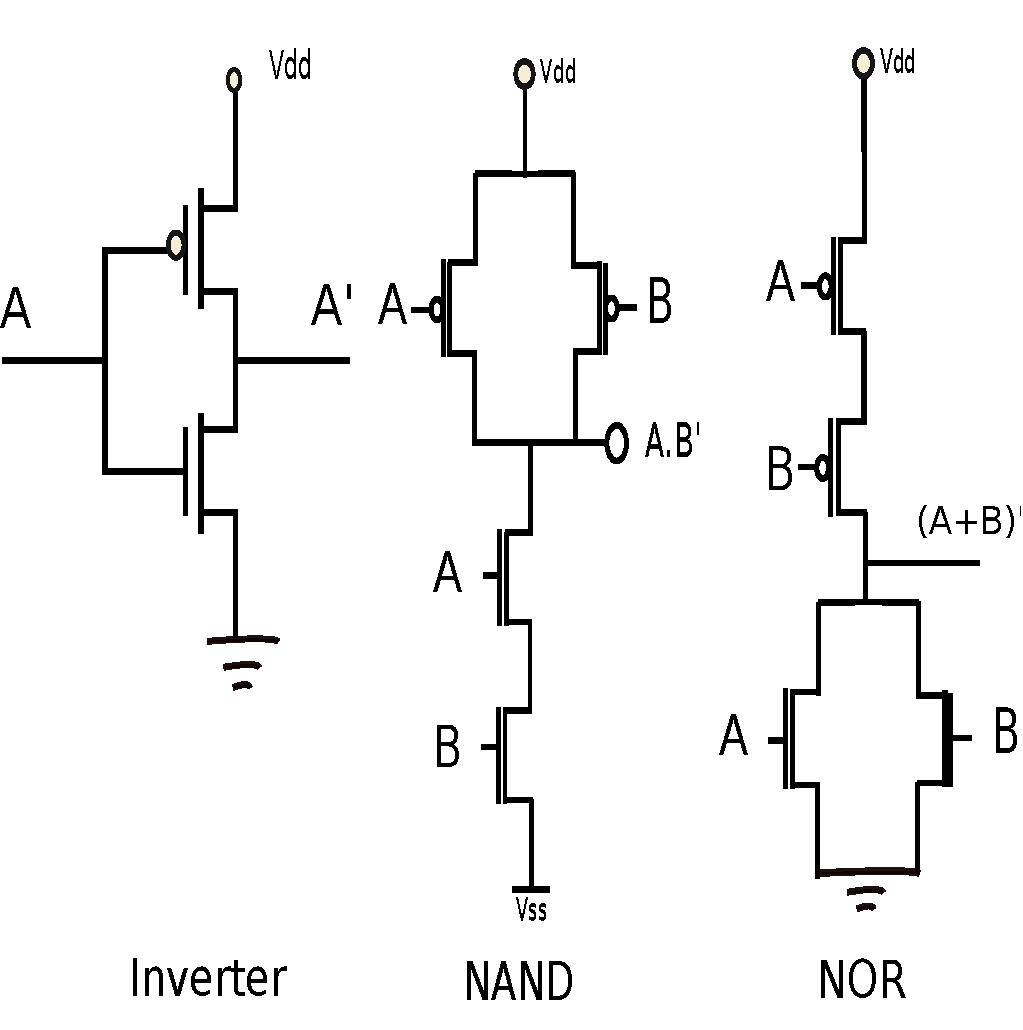
\includegraphics[width=10cm,height=8cm,keepaspectratio]{4.pdf}
\end{figure}
\Exercise
Implement the AND, OR and NOT gates using NAND gates only.
\begin{figure}[H]
  \centering
  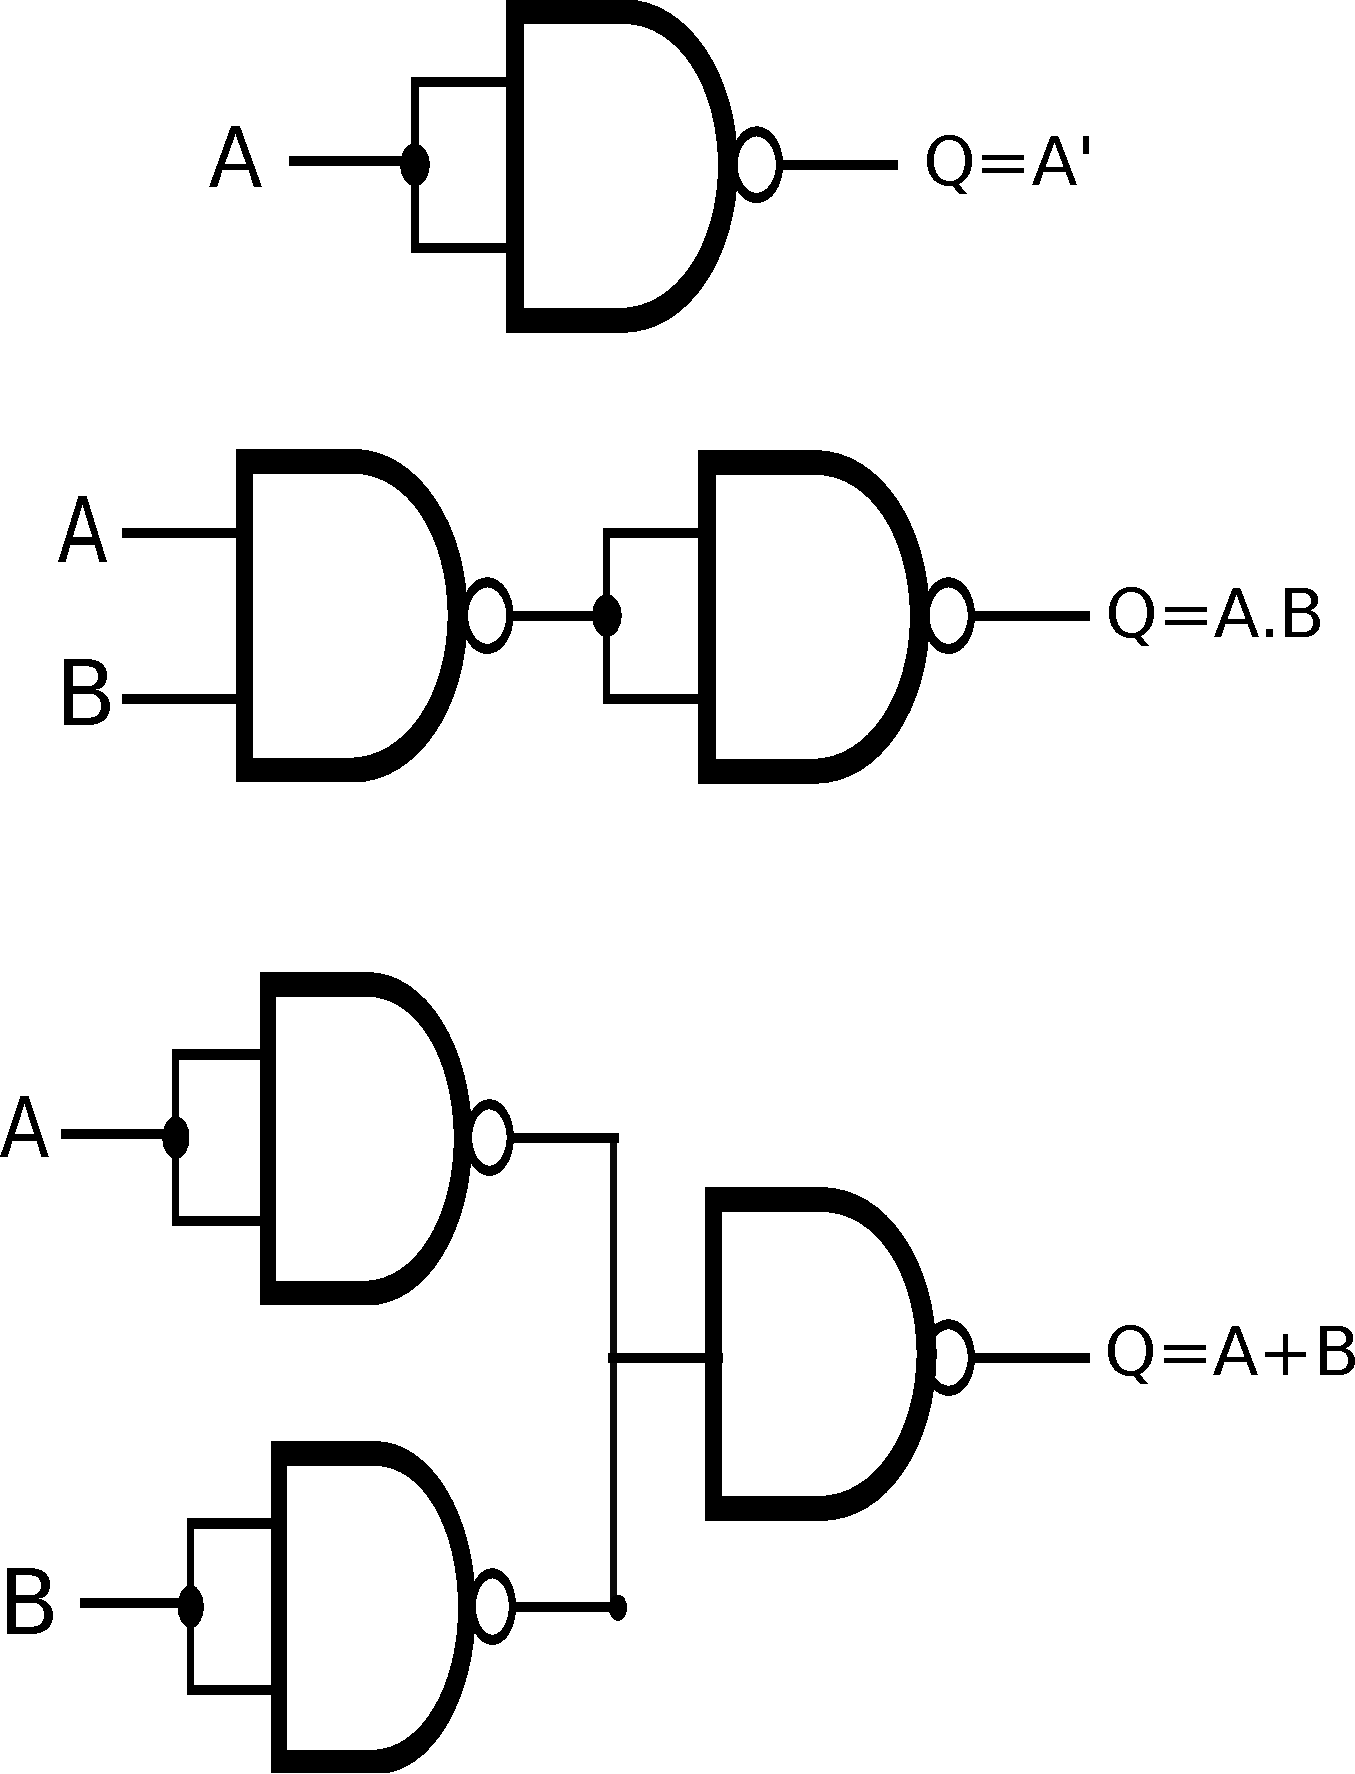
\includegraphics[width=10cm,height=8cm,keepaspectratio]{5.pdf}
\end{figure}
\Exercise
Implement the AND, OR and NOT gates using NOR gates only.
\begin{figure}[H]
  \centering
  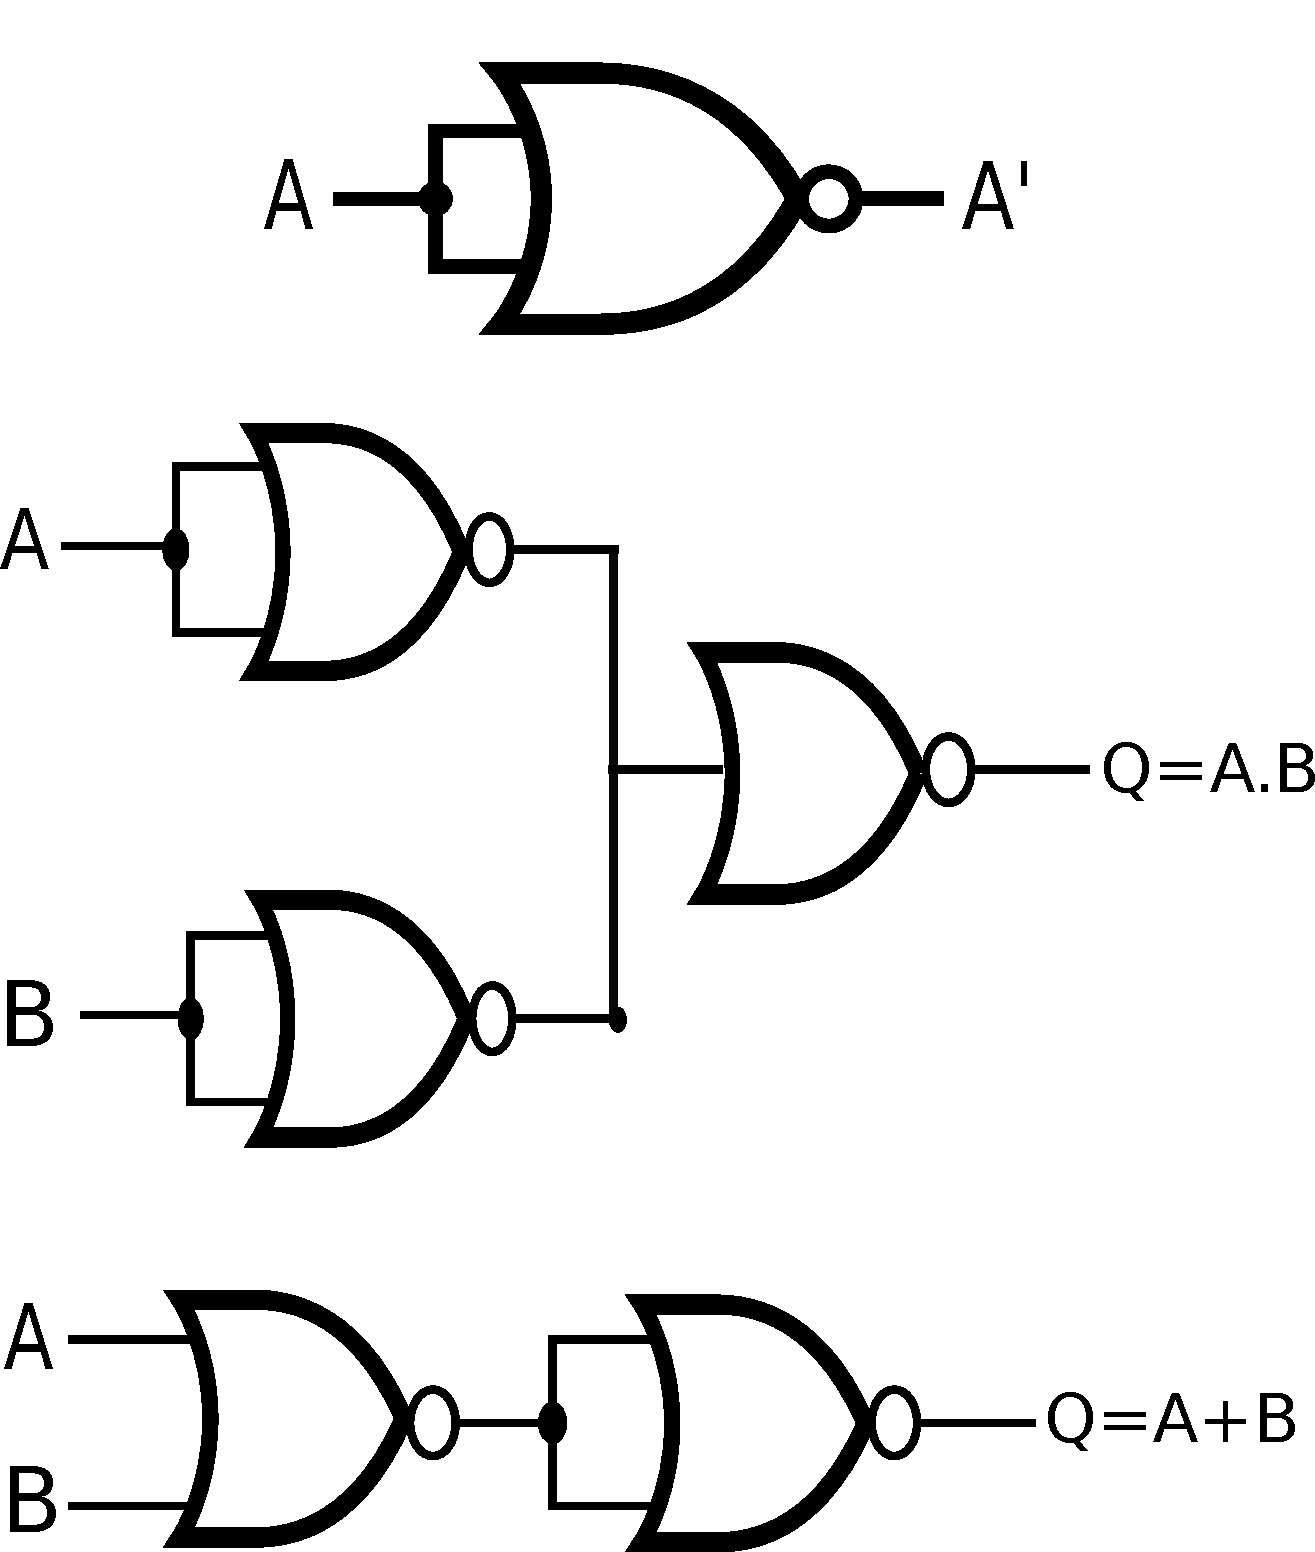
\includegraphics[width=10cm,height=8cm,keepaspectratio]{6.pdf}
\end{figure}
\Exercise
Implement XOR and XNOR gates using NAND gates only.
\begin{figure} [H]
  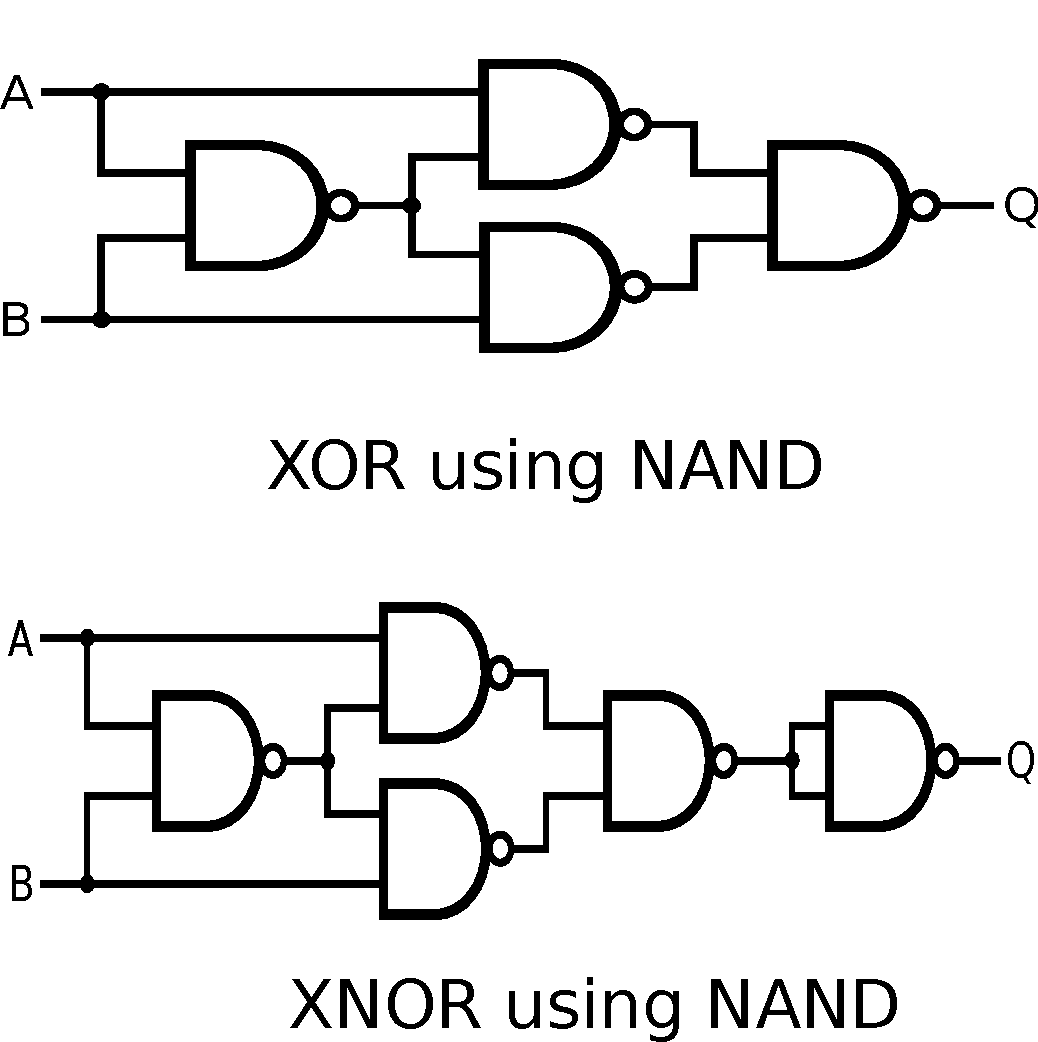
\includegraphics[width=10cm,height=8cm,keepaspectratio]{7xor.pdf}
\end{figure}

\Exercise
\label{que:gatec}
Implement the following Boolean functions by using only AND, OR and NOT gates.
\begin{enumerate}[ a) ]
\item
$\overline A .B + A.\overline B + \overline A.\overline B.\overline C$
\item
$\overline{(A+B+C)}.(\overline A.\overline B+C)$
\item
$\overline{(A+B)}.\overline{(\overline C+\overline D)}$
\item
$\overline A.\overline B.\overline C + A.B.C + \overline D$
\end{enumerate}
a)
\begin{figure} [H]
  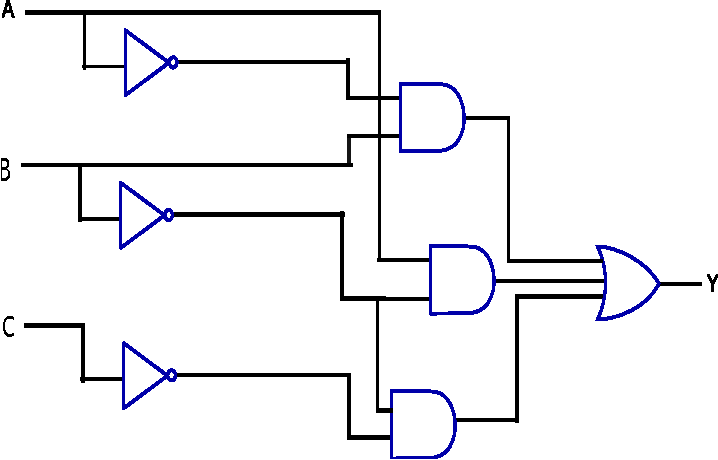
\includegraphics[width=10cm,height=8cm,keepaspectratio]{8a.pdf}
\end{figure}
b)\begin{figure} [H]
  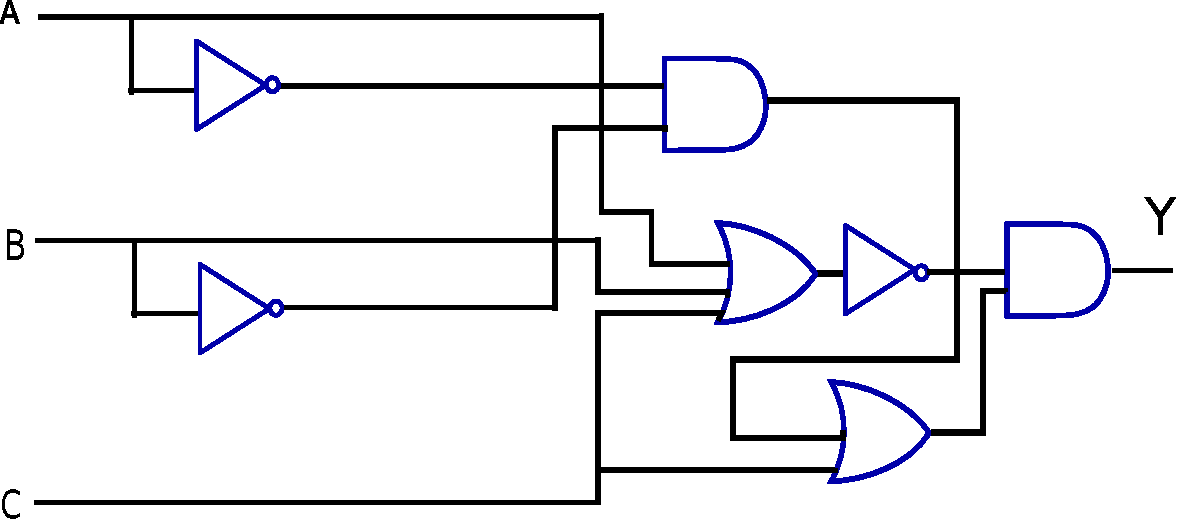
\includegraphics[width=10cm,height=8cm,keepaspectratio]{8b.pdf}
\end{figure}
c)\begin{figure} [H]
  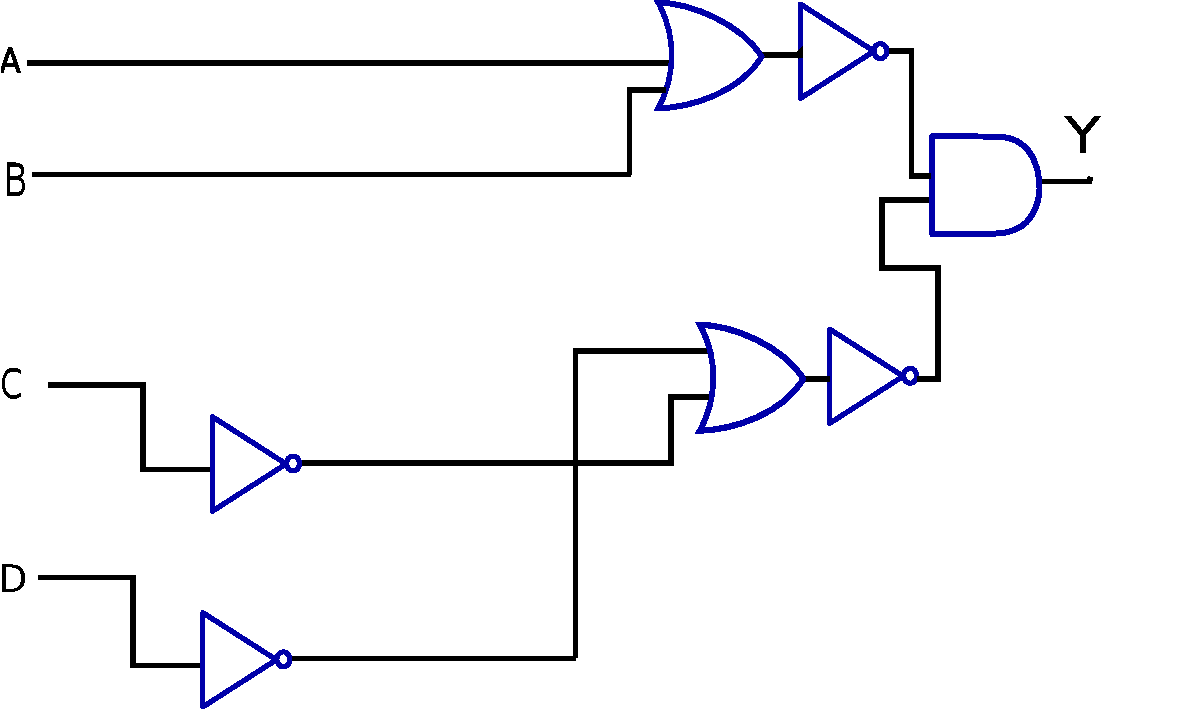
\includegraphics[width=10cm,height=8cm,keepaspectratio]{8c.pdf}
\end{figure}
d)\begin{figure} [H]
  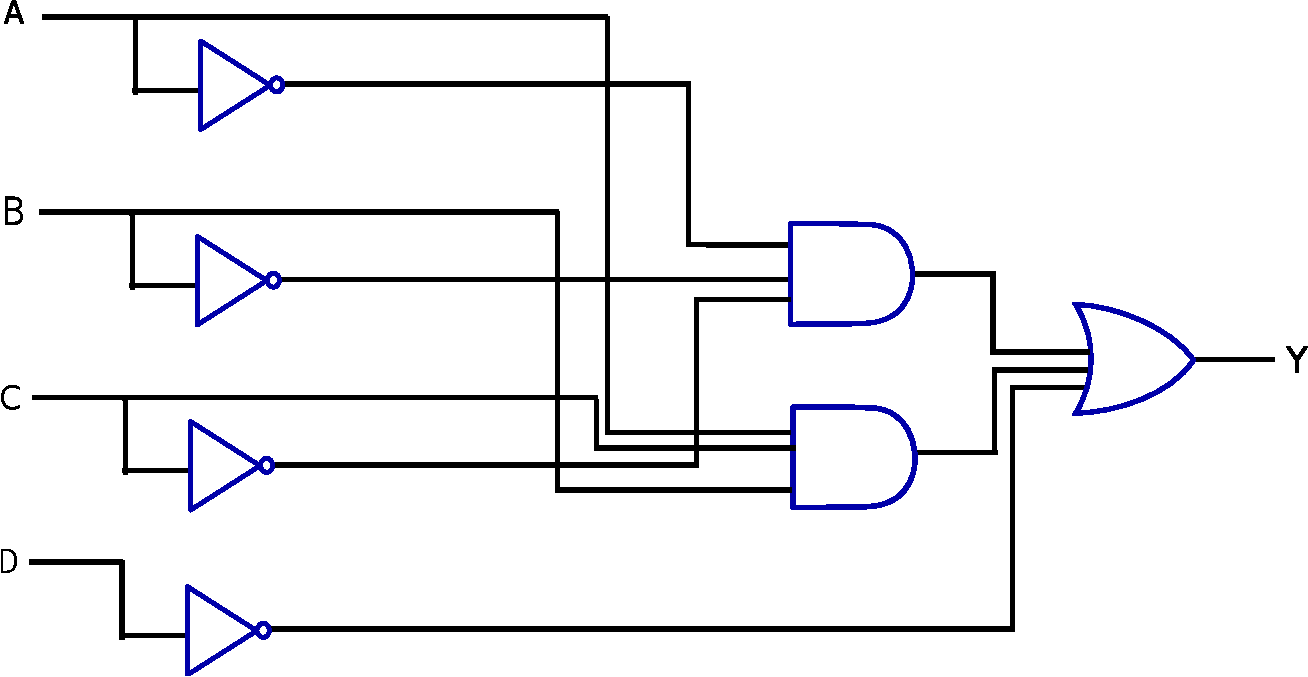
\includegraphics[width=10cm,height=8cm,keepaspectratio]{8d.pdf}
\end{figure}

\Exercise
Answer Question~\ref{que:gatec} by using only NAND gates.

\Answer
a)
\begin{figure} [H]
  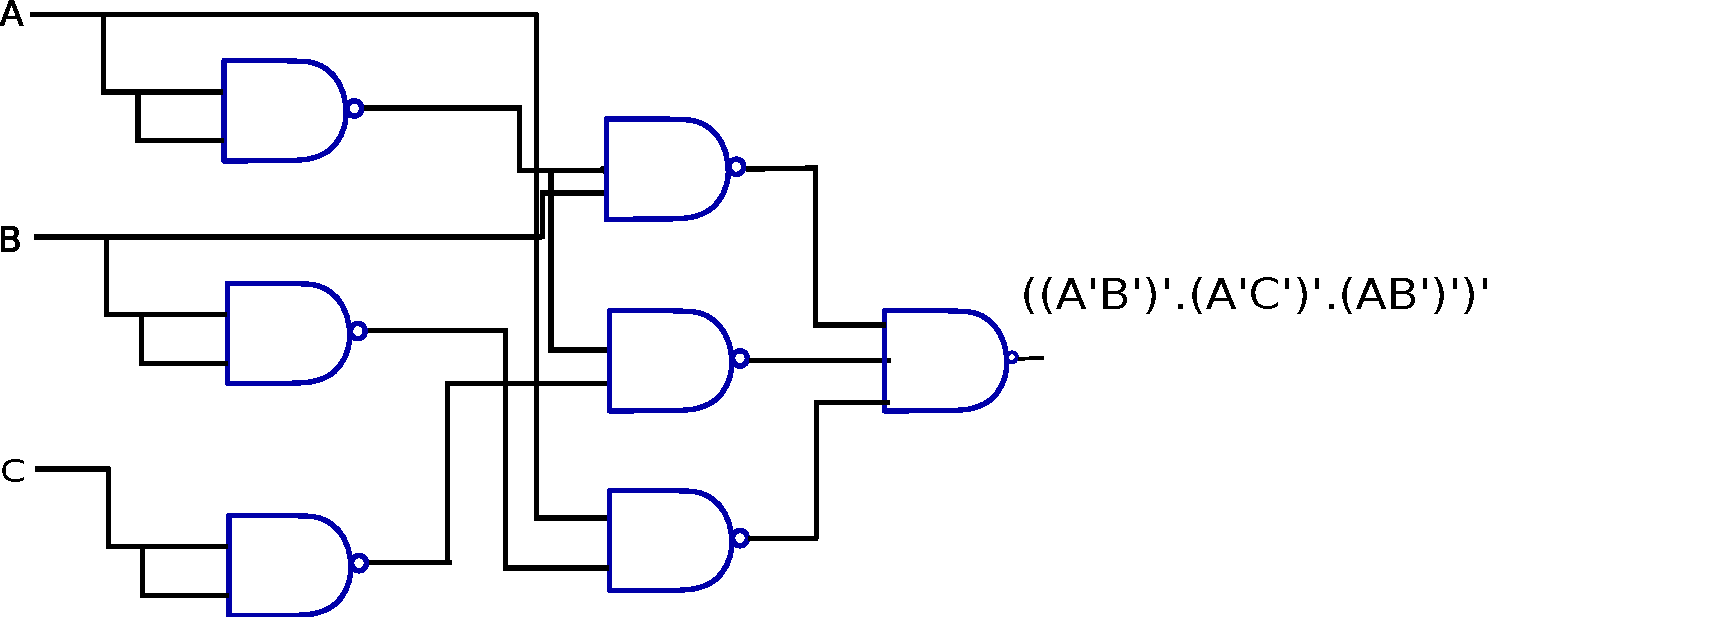
\includegraphics[width=10cm,height=8cm,keepaspectratio]{9a.pdf}
\end{figure}
b)\begin{figure} [H]
  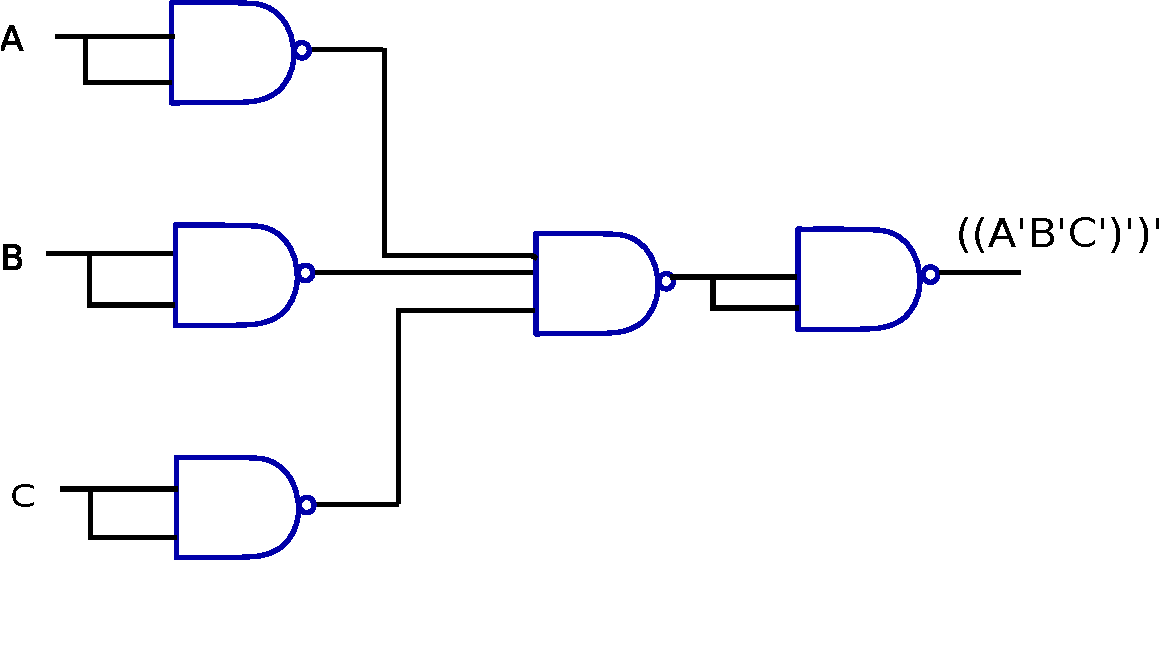
\includegraphics[width=10cm,height=8cm,keepaspectratio]{9b.pdf}
\end{figure}
c)\begin{figure} [H]
  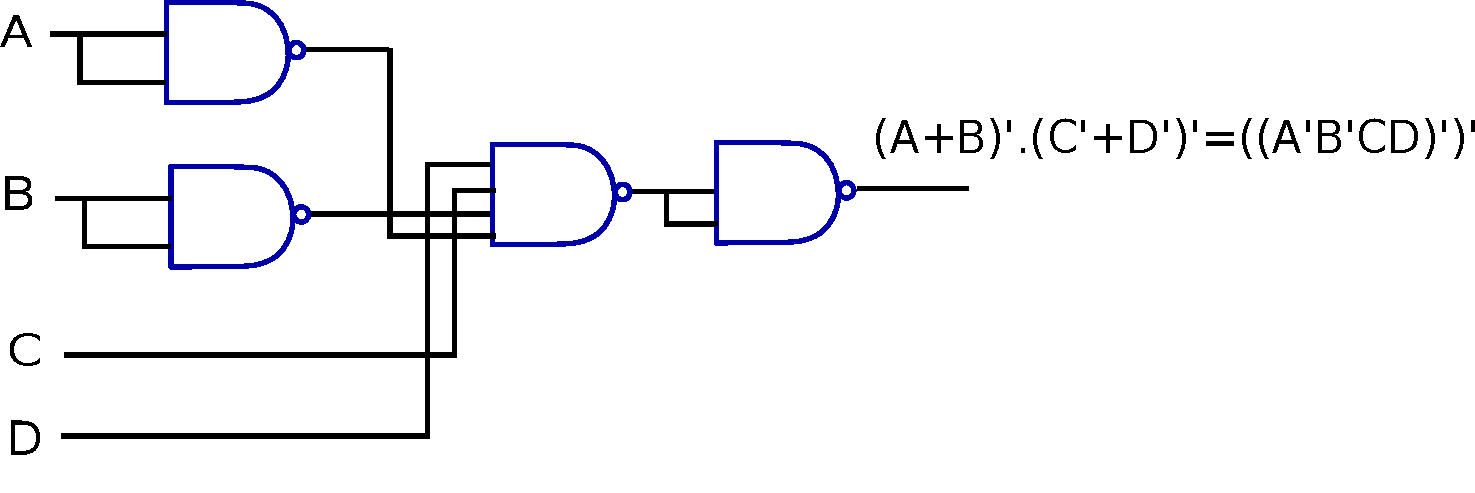
\includegraphics[width=10cm,height=8cm,keepaspectratio]{9c.pdf}
\end{figure}
d)\begin{figure} [H]
  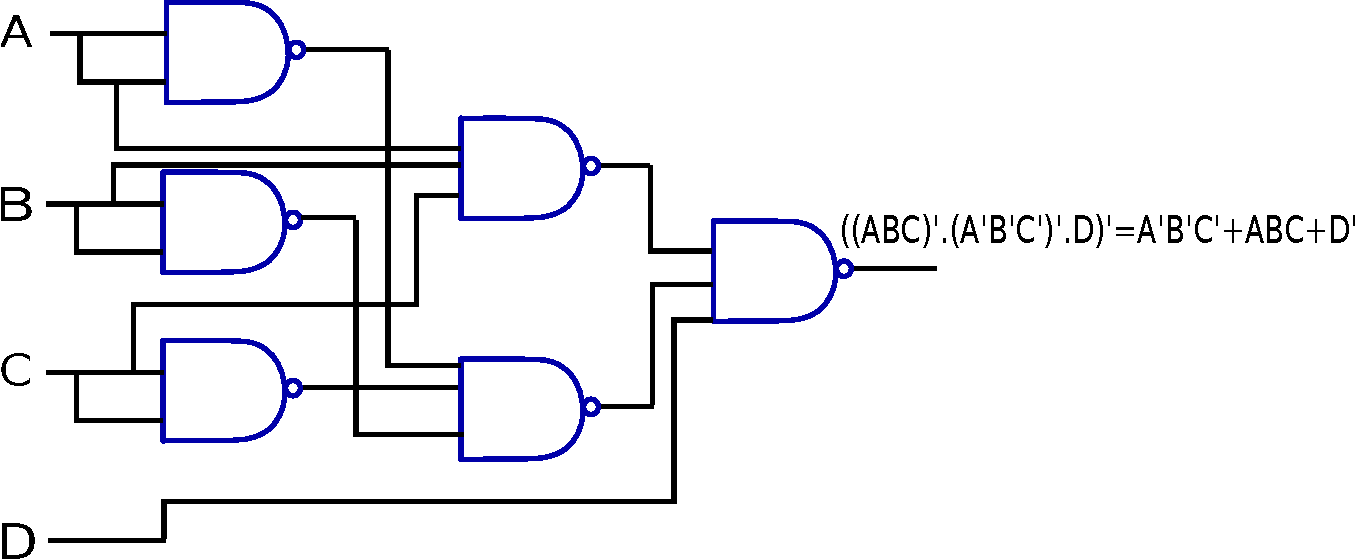
\includegraphics[width=10cm,height=8cm,keepaspectratio]{9d.pdf}
\end{figure}

\end{ExerciseList}

\subsection*{Combinational Logic and Sequential Logic}

\begin{ExerciseList}
\Exercise
Draw the circuit diagram of a $3 \times 8$  decoder.

\begin{figure} [H]
  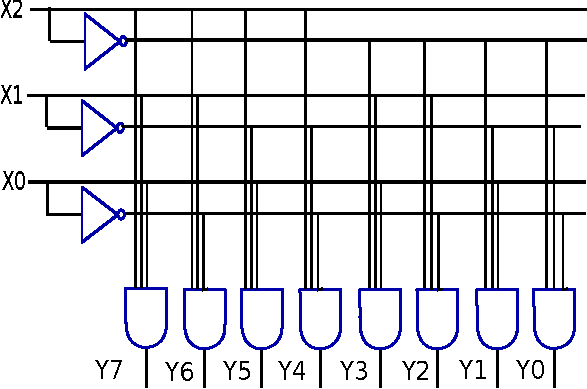
\includegraphics[width=10cm,height=8cm,keepaspectratio]{10.pdf}
\end{figure}
\Exercise
Draw the circuit diagram of a $8-3$ bit encoder.

\begin{figure} [H]
  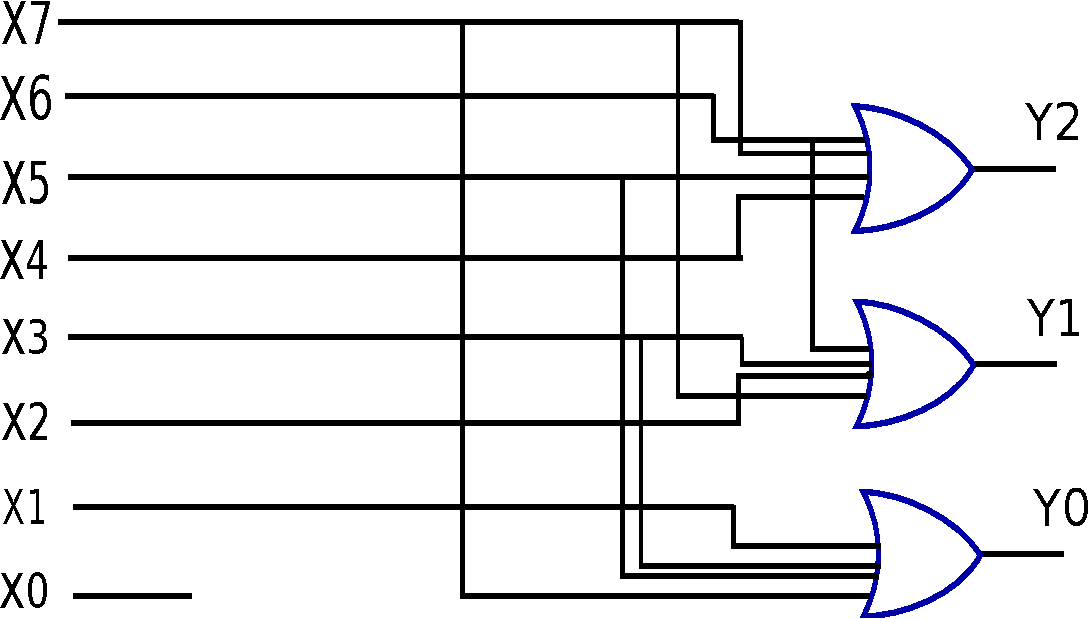
\includegraphics[width=10cm,height=8cm,keepaspectratio]{11.pdf}
\end{figure}

\Exercise
Draw the circuit diagram of a $8-3$ bit priority encoder.
\begin{figure} [H]
  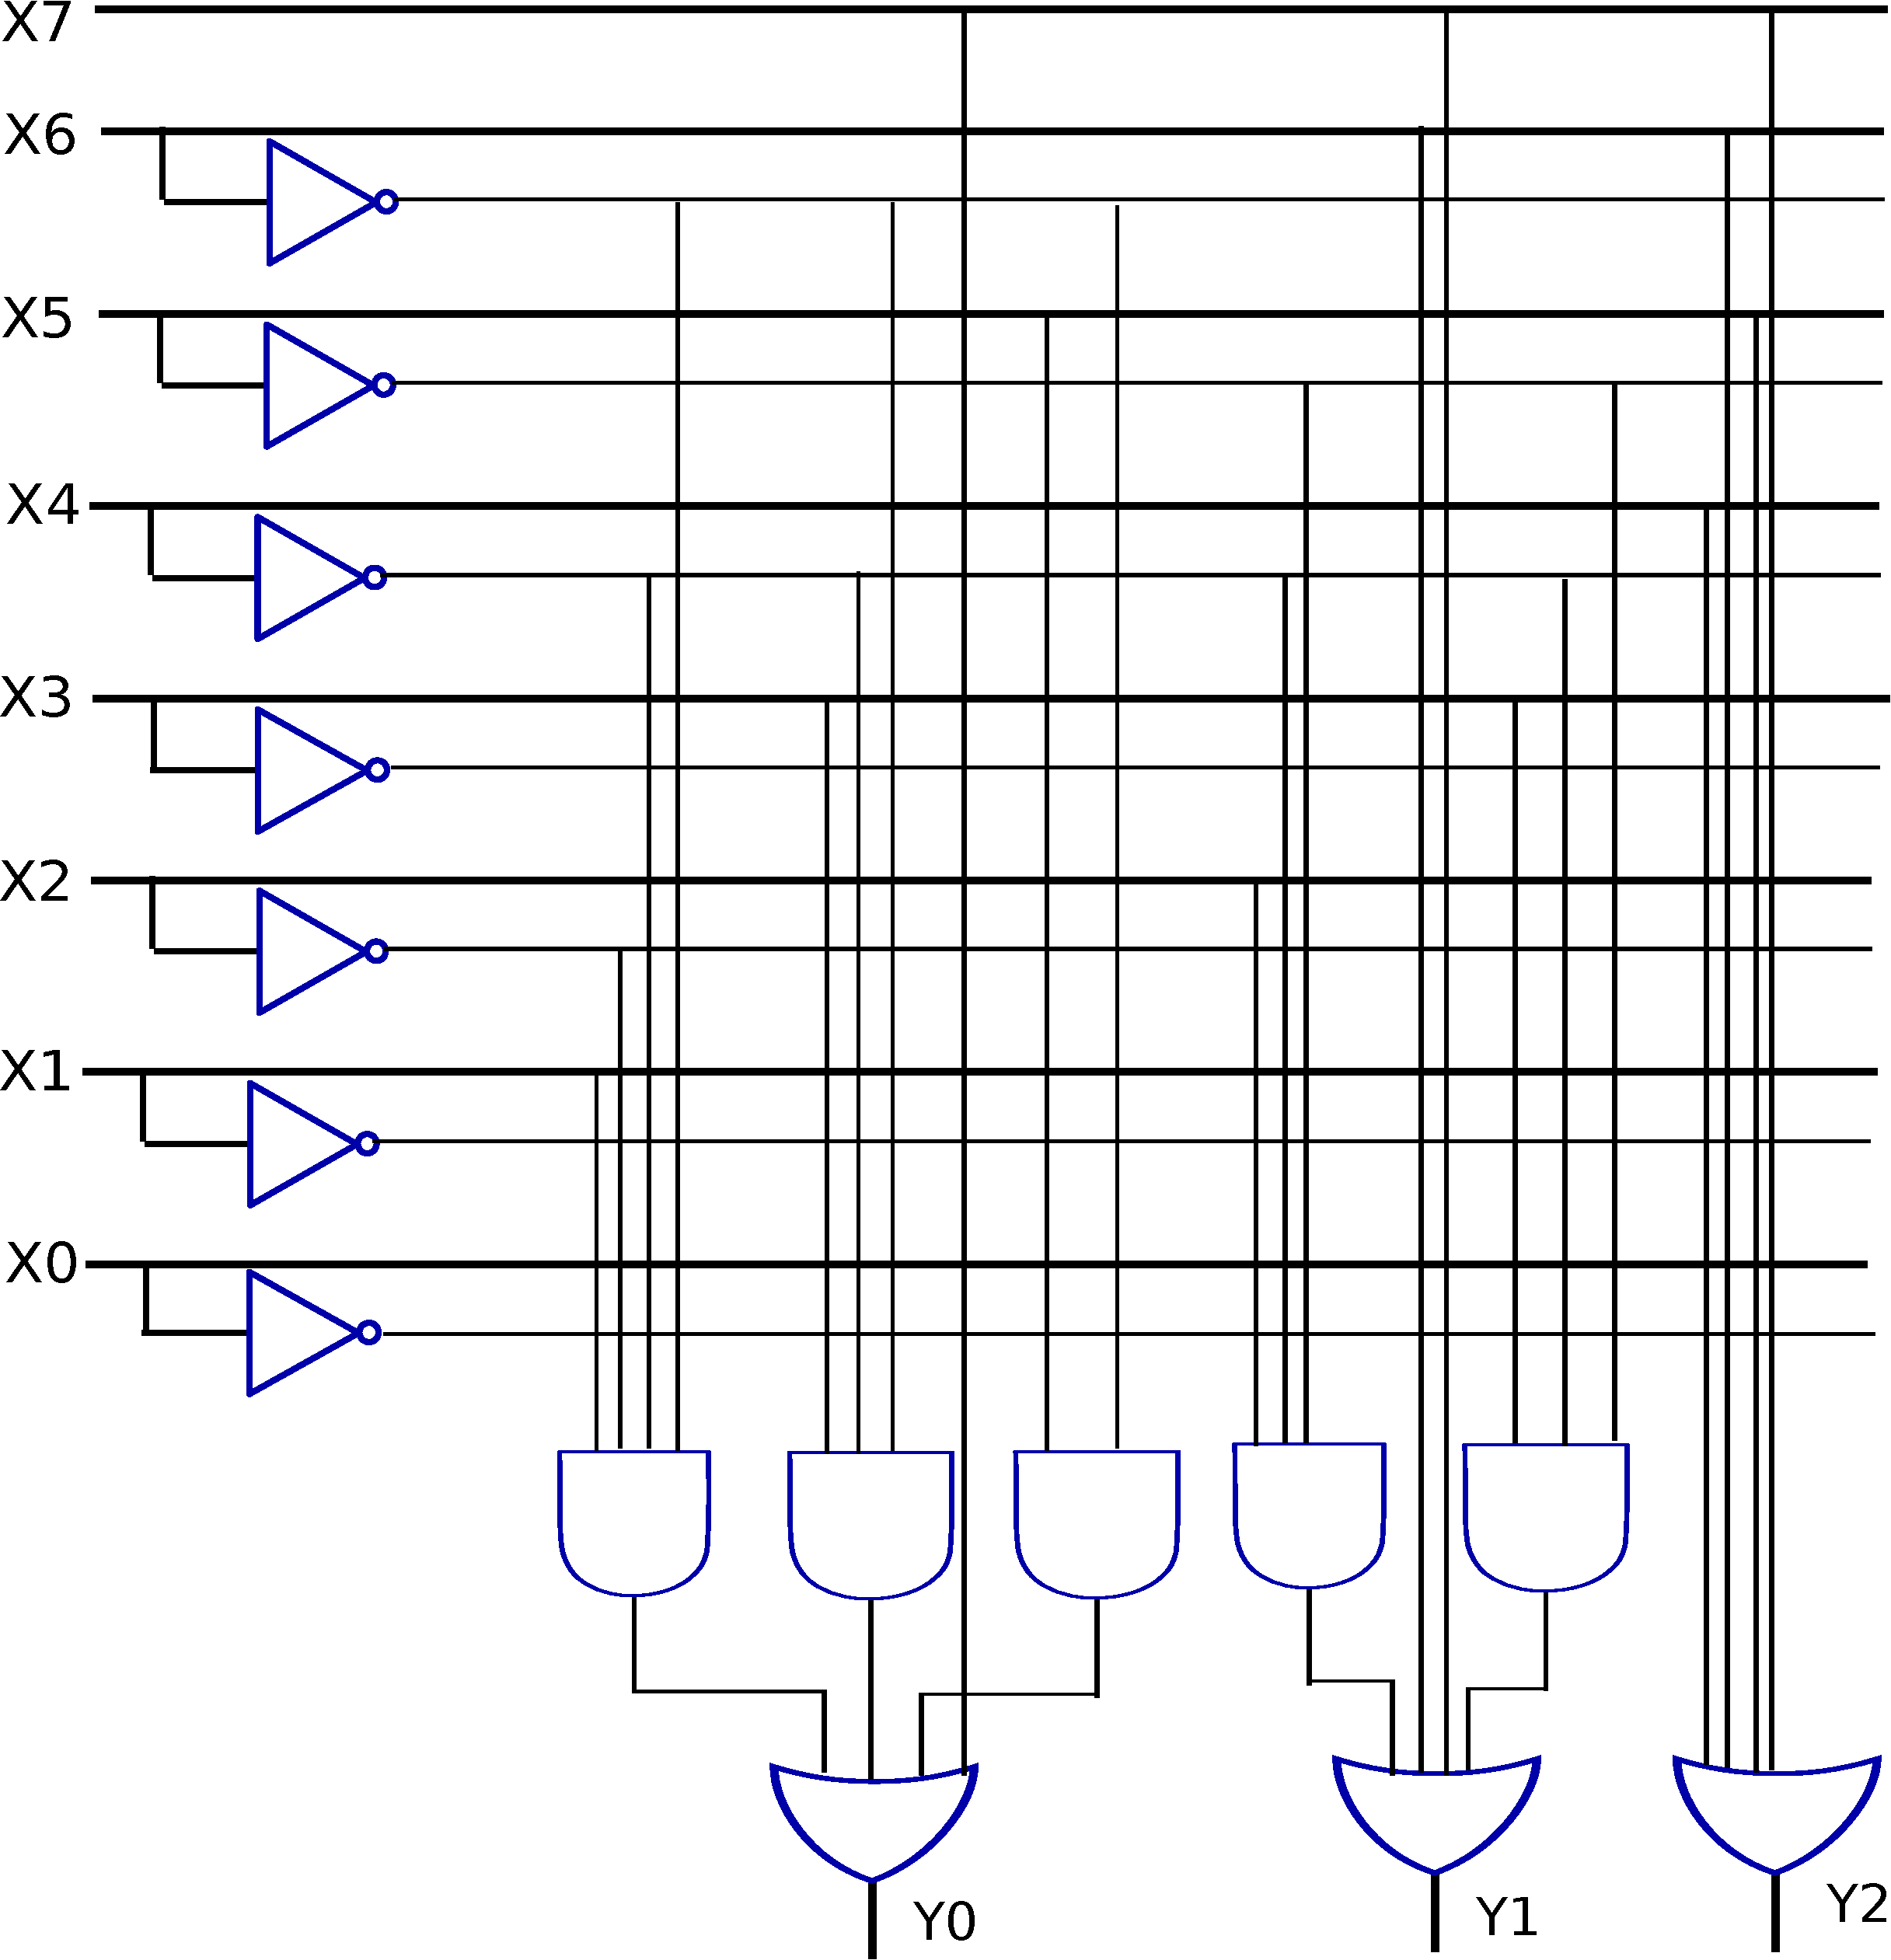
\includegraphics[width=10cm,height=10cm,keepaspectratio]{12.pdf}
\end{figure}

\Exercise
Suppose a poll has to be conducted with three entities A, B and C, each of which can
either vote a `yes' (encoded as 1) or a `no' (encoded as 0). The final output
is equal to the majority opinion. Draw a truth table of the
system, simplify the function, and implement it using logic gates.
\Answer $\newline$

\begin{figure} [H]
  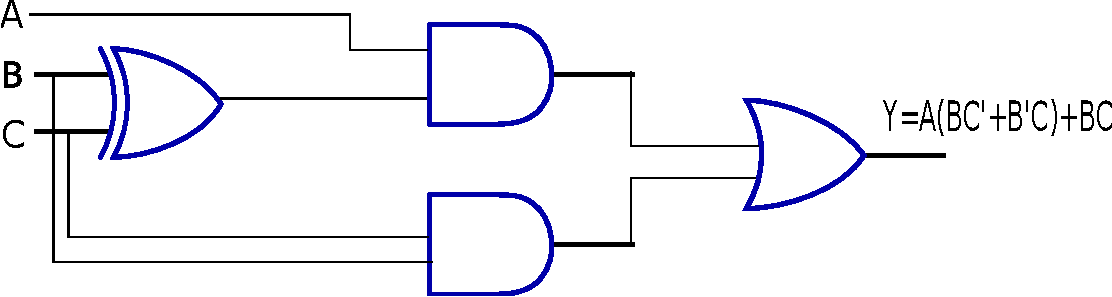
\includegraphics[width=10cm,height=10cm,keepaspectratio]{13.pdf}
\end{figure}



\begin{tabu} to 0.4\textwidth { | X[l] | X[c] | X[cr] |X[r]|}
 \hline
 A & B & C & Y \\
 \hline
 0 & 0 & 0 & 0\\
\hline
 0 & 0 & 1 & 0\\
\hline
 0 & 1 & 0 & 0\\
\hline
 0 & 1 & 1 & 1\\
\hline
 1 & 0 & 0 & 0\\
\hline
 1 & 0 & 1 & 1\\
\hline
 1 & 1 & 0 & 1\\
\hline
 1 & 1 & 1 & 1\\
\hline
\end{tabu}\\

$Y= \overline A BC + A \overline BC + AB\overline C +ABC\newline
 =BC + A(\overline B C+B\overline C) \newline$
 
\Exercise[difficulty=1]
Most circuits in modern computers are built using NAND and NOR gates, because
they are easy to build using CMOS technology.
Suppose another
technology in invented in the near future, 
which implements a new gate, $X$, very efficiently. $X$ takes 3
inputs $A$, $B$ and $C$ and computes:
 $X(A,B,C) = A.B + \overline C$.
Using only X gates and NOT gates, how will you implement the following function:
$f(A,B,C) = A+B+C$?


\Answer
$A+B = X(A,1,\overline B )\\
A+B+C = X(A+B, 1, \overline C )\\
\Rightarrow A+B+C = X(X(A,1,\overline B ),1,\overline C)$

\Exercise[difficulty = 2]
Implement the following logic functions using a 4 to 1 multiplexer, and a single
NOT gate.

\begin{enumerate}[(a) ]
\item
$AB + BC + AC$
\item
$\overline A + \overline B + \overline C$
\item
$A.\overline B + A.B.\overline C$
\end{enumerate}

\Answer 
a)\begin{figure}[H]
  \centering
  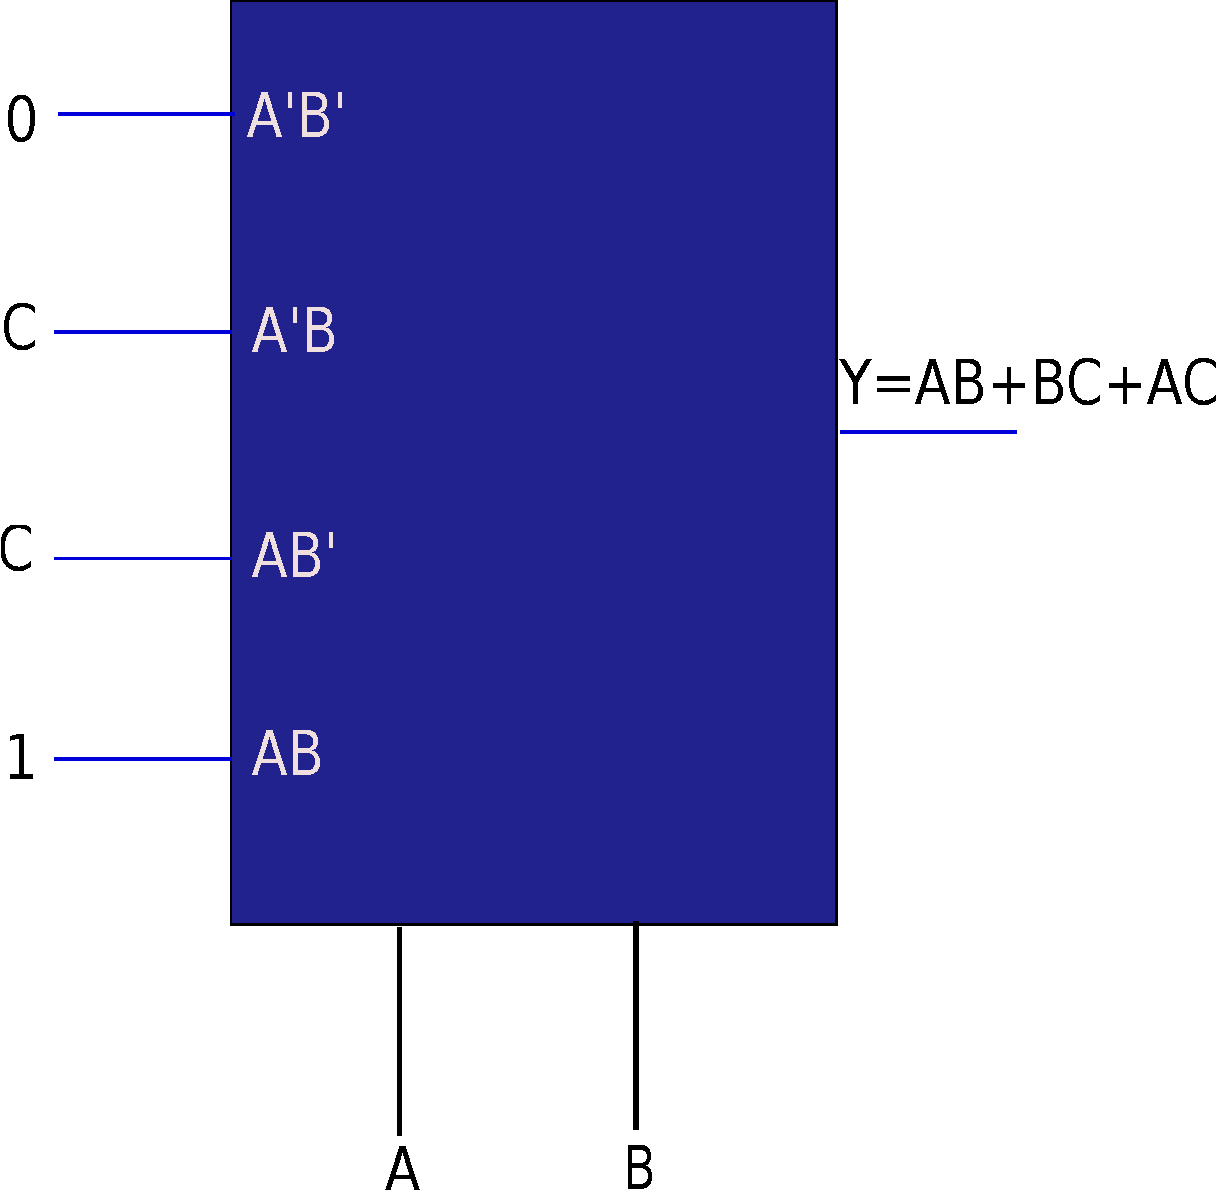
\includegraphics[width=10cm,height=8cm,keepaspectratio]{15a.pdf}
\end{figure}

b)\begin{figure}[H]
  \centering
  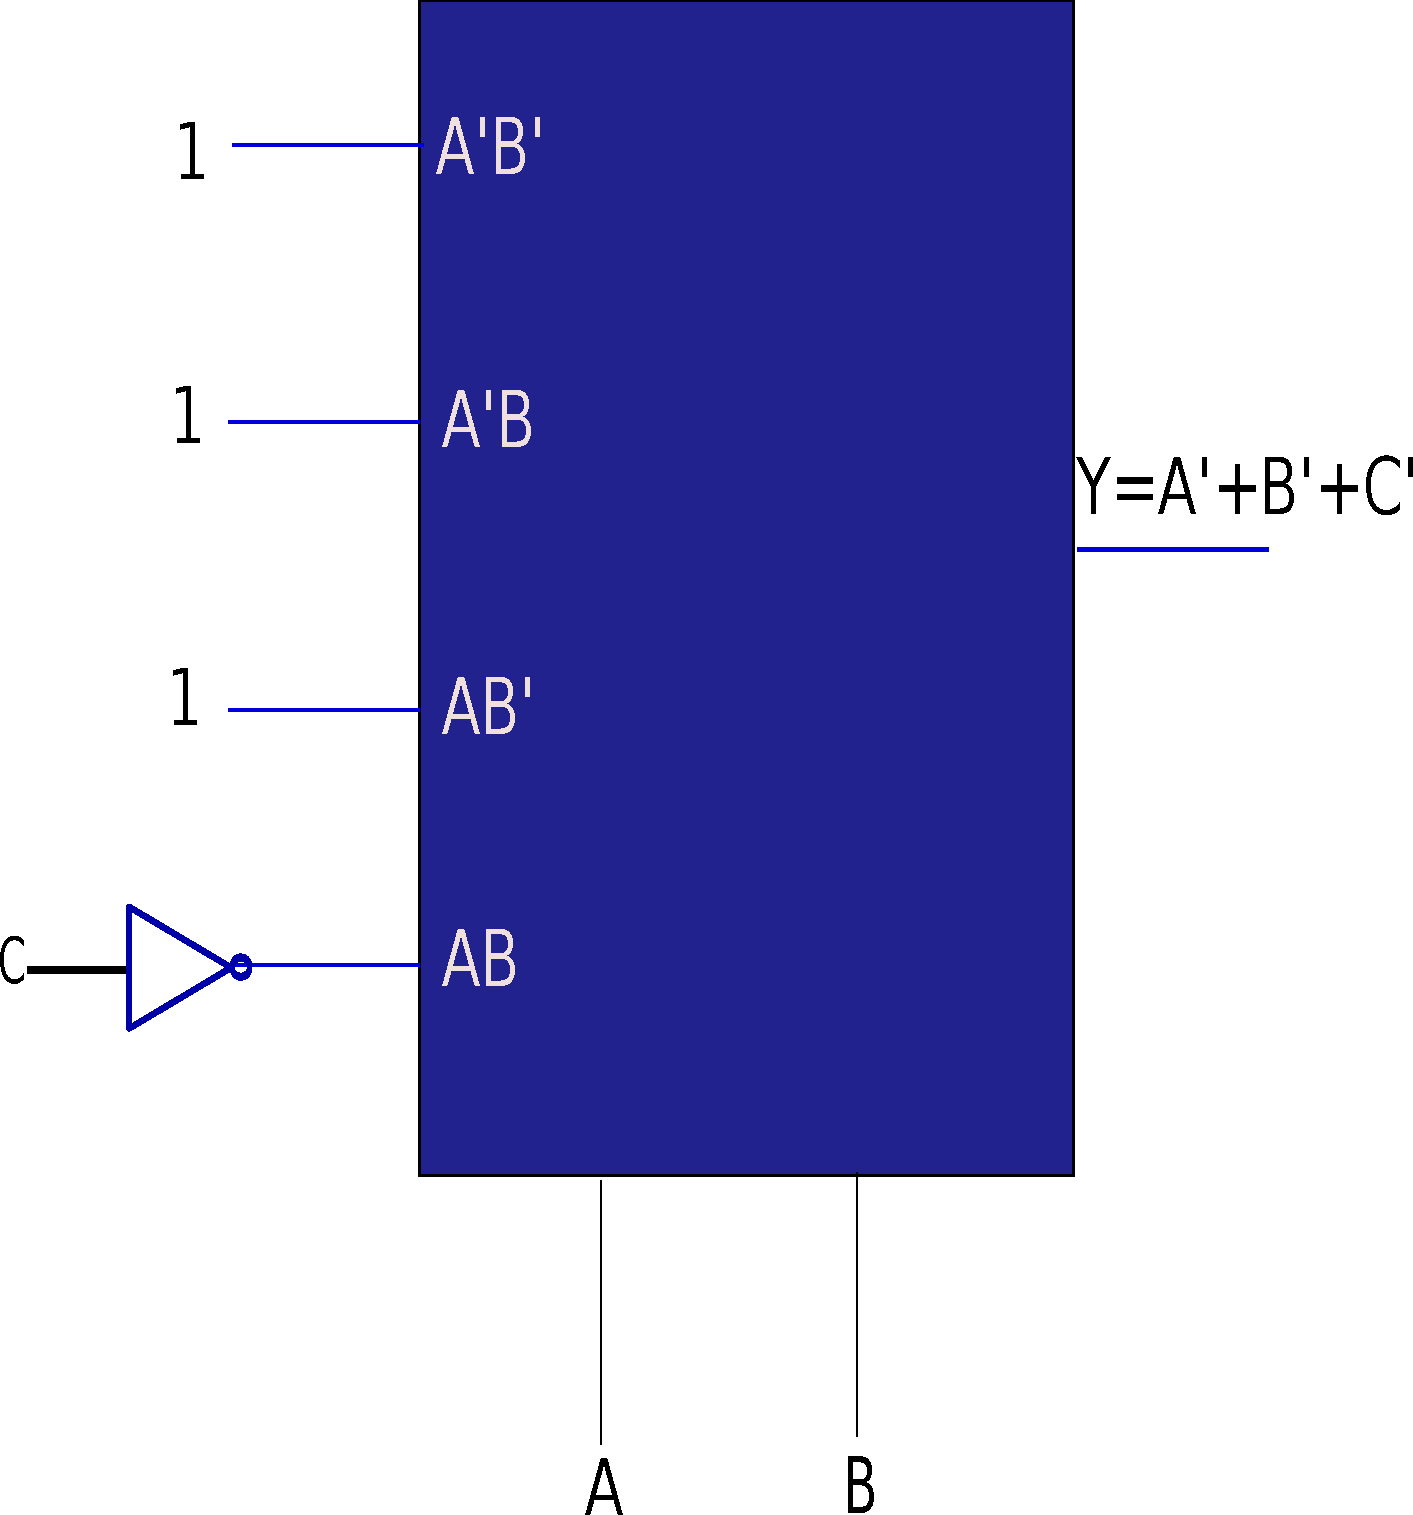
\includegraphics[width=10cm,height=8cm,keepaspectratio]{15b.pdf}
\end{figure}

c)\begin{figure}[H]
  \centering
  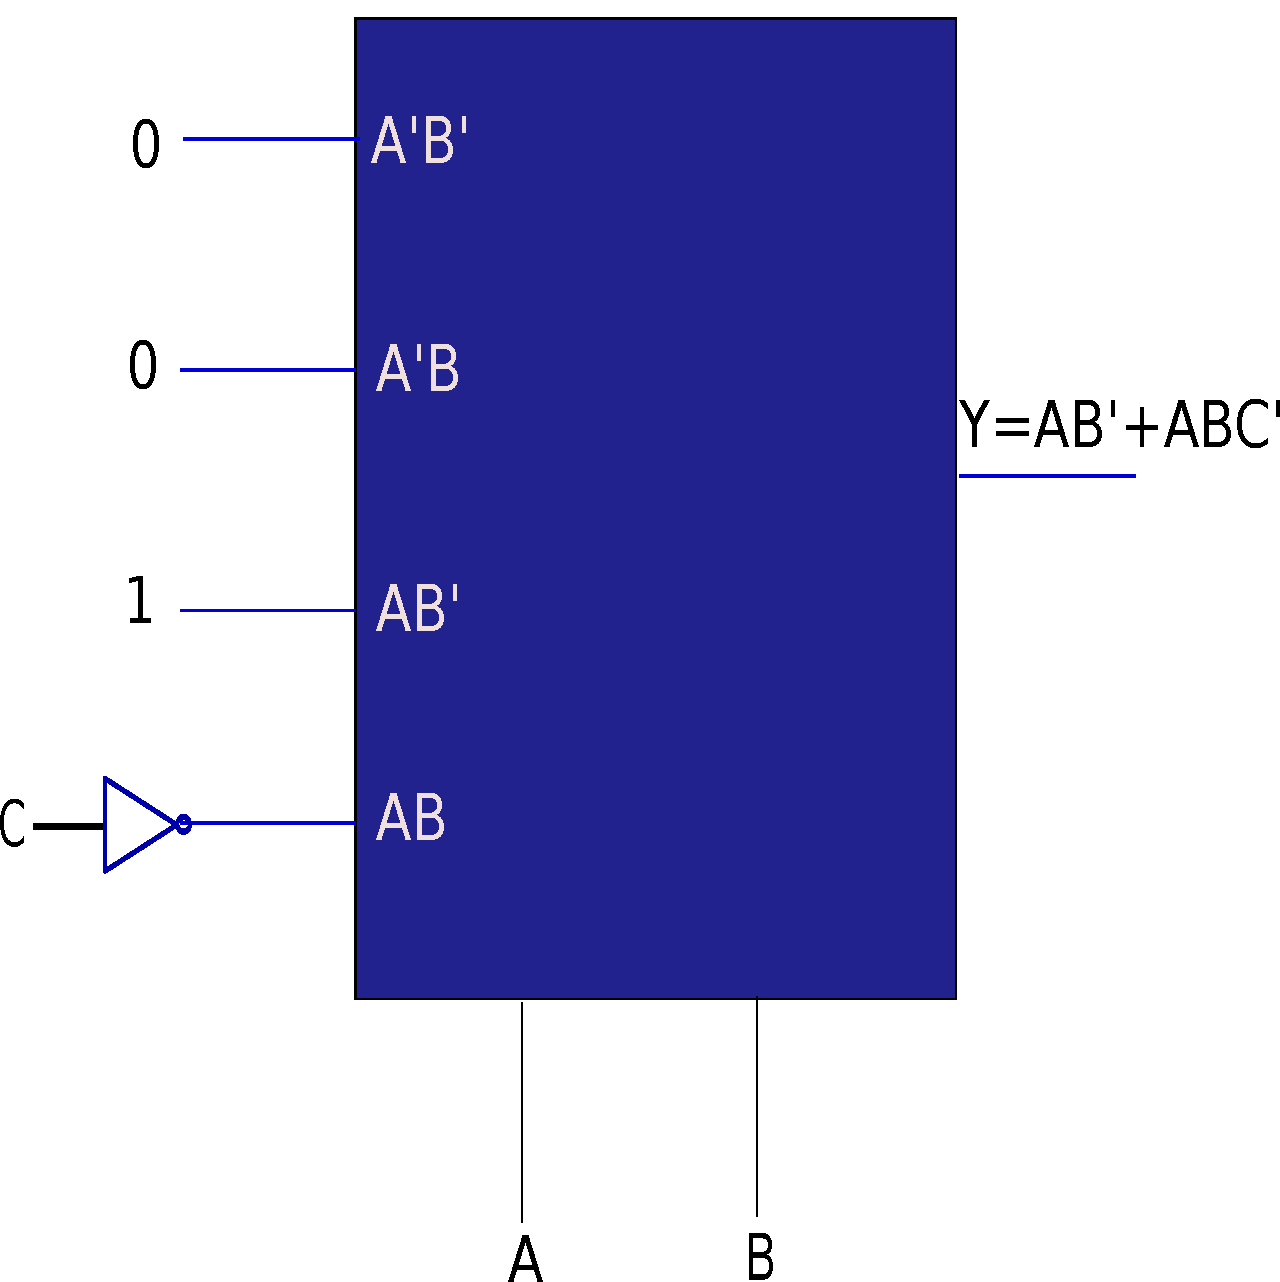
\includegraphics[width=10cm,height=8cm,keepaspectratio]{15c.pdf}
\end{figure}
\Exercise[difficulty=2]
Is it possible to implement every 3 variable Boolean function with a 4 to 1 multiplexer,
and a single NOT gate? Prove your answer.

\Answer
Yes, it is possible.Let $F(A,B,C)$ be the function we want to implement using a $4\times 1$
MUX. The range of this function is \{0, 1\}. We can now define an equivalent
$G(A,B)$ with range \{0, 1, $C$, $\overline C$\} such that for for each given
$A$, $B$ and $C$, $F(A,B,C) = G(A,B)$ . Now giving $A$ and $B$ to the control
lines of the multiplexer, the data lines can be set accordingly , using the truth table to give the correct output. This is possible for every 3 variable Boolean function as every $F(A,B,C)$ can be expressed as $G(A,B)$ which takes only one of the four values - \{0, 1, $C$, $\overline C$\} . Thus, the aforesaid implementation is possible.

\end{ExerciseList}

\section*{Sequential Logic}

\begin{ExerciseList}
\Exercise
What is the difference between a flip-flop and a latch?
\Answer 
1. Latch continuously checks its inputs and changes outputs accordingly. A flip-flop on the other hand, checks its inputs and changes outputs correspondingly, only at times determined by the clocking signal.\\
2. A latch is level-triggered, that is the value of the output is determined at each level of the clock pulse. A flip-flop is edge triggered, that is the output is determined at either the positive/negative edge of the clock pulse. \\
\Exercise
Define the following terms:
\begin{enumerate}[i)]
\item Setup time
\item Hold time
\item Metastability
\item {\em Keep out} region
\end{enumerate}
\Answer 
\hspace{3mm} \\
a) \textit{Setup time}: The units of time for which the input is desired to be kept stable before the triggering of the clock pulse is called \textit{setup time}. \\
b) \textit{Hold time}: The units of time for which the input is desired to be kept stable after the triggering of the clock pulse is called \textit{hold time}. \\
c) \textit{Metastability}: The phenomenon in which the output of a flip-flop becomes non-deterministic, fluctuating and oscillating due to a change in the input during positive/negative edge of the clock, depending on the type of edge-triggering, is called \textit{metastability}. \\
d) \textit{Keep-out region}: The window of time during which it is desired to keep the inputs stable is called \textit{keep-out region}. \\
\Exercise
Why do we wish to avoid the indeterminate state in an S-R flip-flop?
\Answer
The SR flip-flop using NAND gates gives an indeterminate output when both S and R are equal to 1. We need to avoid this as it may result in a race condition, and the output can become unpredictable. The output keeps oscillating/fluctuating between 0 and 1. 
\Exercise
What is the advantage of an edge sensitive flip-flop?
\Answer
In a level sensitive flipflop, circuits have half a clock cycle to compute the correct outputs ie: when the clock is 0. When the clock is 1 (high), the outputs are visible. In an edge sensitive flip-flop, changes are visible only at the upward/downward edge of a clock. This gives us more accurate results since a unique well-defined point is needed for determination of accurate outputs. Also, an edge sensitive flip-flop gives one full cycle for computation of correct outputs. Another issue is with the circuits that have feedback (the outputs are connected back to the inputs) where level triggering causes chaos, because the level is wide enough (half a clock cycle) that the output can feed back to the inputs within the same period, and output becomes unpredictable.     \\
\Exercise[difficulty = 1]
What is the fundamental advantage of a JK flip-flop over a D flip-flop? 
\Answer
The fundamental advantage is that a JK flip-flop is used for toggling by shorting the inputs J and K and giving it a logical 1. The D flipflop has only (J=1 and K=0 and viceversa) states when enabled, and latches the previous state values when disabled. Thus, a JK flip-flop can be used like a D flip-flop with toggling.
 
\Exercise
Describe the design of registers in your own words.
\Answer
Registers are groups of flip-flops, where each flip-flop is capable of storing one bit of information. An $n$-bit register is a group of n flip-flops. The basic function of a register is to hold information in a digital system and make it available to the logic elements for the computing process. Registers consist of a finite number of flip-flops. Since each flip-flop is capable of storing either a "0" or a "1", there is a finite number of 0-1 combinations that can be stored into a register. Each of those combinations is known as state or content of the register. There are many types of registers: \\
1. \textit{Parallel-in Parallel out}: \\
This can be designed using D flipflops where each D flipflop is connected to an input line. The $n$ bits are loaded in parallel to each of the $n$ D flipflops and are also read out in parallel at every negative or positive clock edge. \\
2. \textit{Serial-in Parallel out}: \\
This can be designed using D flipflops, where we have a single input that is fed to the leftmost D flip-flop. Every cycle, the input moves to the adjacent flip-flop on the right. Thus, in order to load $n$ bits, it takes $n$ cycles. The first bit will get loaded into the leftmost flipflop in the first cycle, and it will take $n$ cycles for it to reach the last flipflop. Then, the output is taken by reading all the $n$ bits in parallel. This is also known as \textit{shift} register. \\

\Exercise
An edge sensitive toggle flip-flop (or T flip-flop) is the one which takes a
clock signal and a single input T and toggles its output on every rising (or
falling) clock edge. How will you construct an edge sensitive T flip-flop form
an edge sensitive J-K flip-flop?

\Answer
Short the inputs J and K of J-K flip-flop into a single wire and call it T.
When T=1 (i.e. J=1 and K=1) the output toggles every clock edge (of same
direction), and when T=0 (i.e. J=0 and K=0), the output remains same.

\Exercise[difficulty=1]
Can you create a negative edge triggered D flipflop using two 2 multiplexers, and a NOT gate?
\begin{figure}[H]
  \centering
  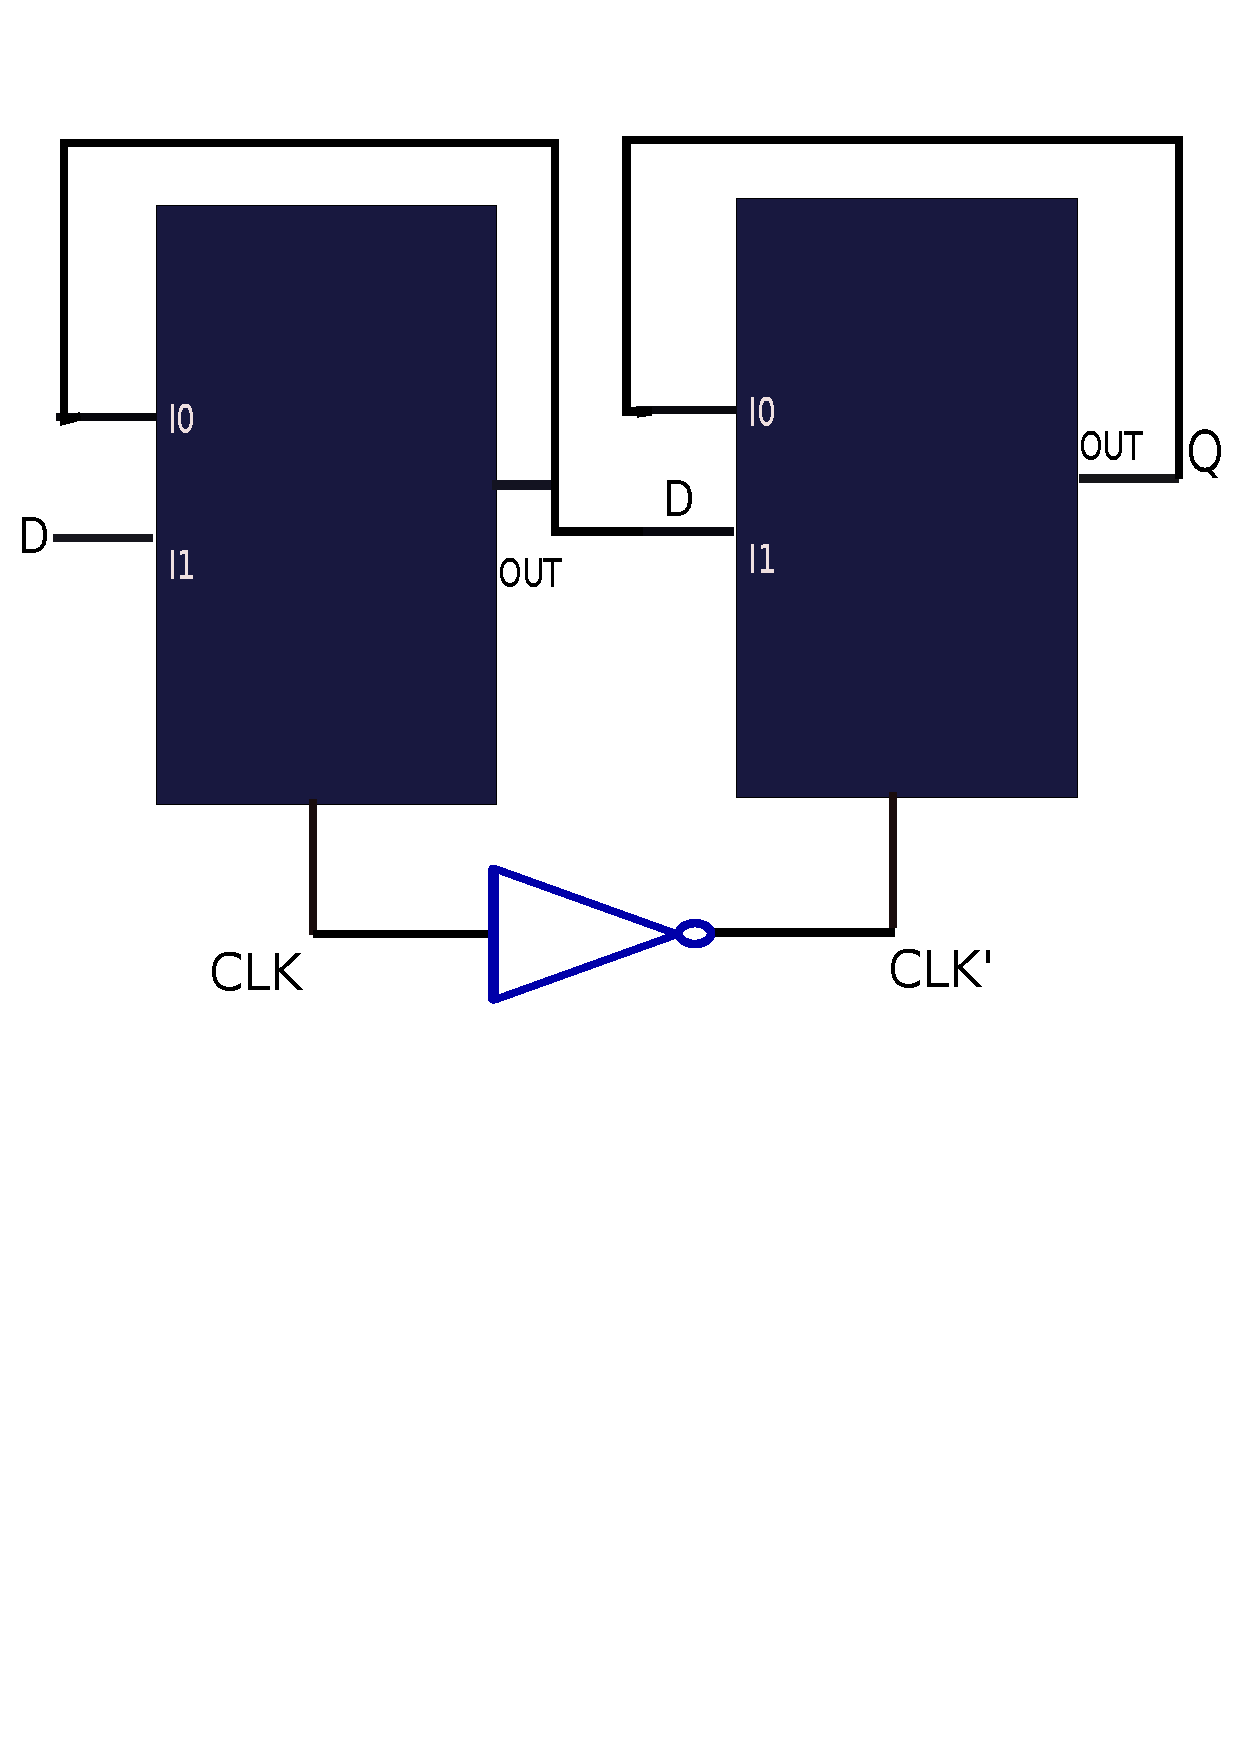
\includegraphics[width=10cm,height=8cm,keepaspectratio]{24.pdf}
  \caption{}
\end{figure}
\Exercise
Design a SR flip-flop with NOR gates.
\begin{figure}[H]
  \centering
  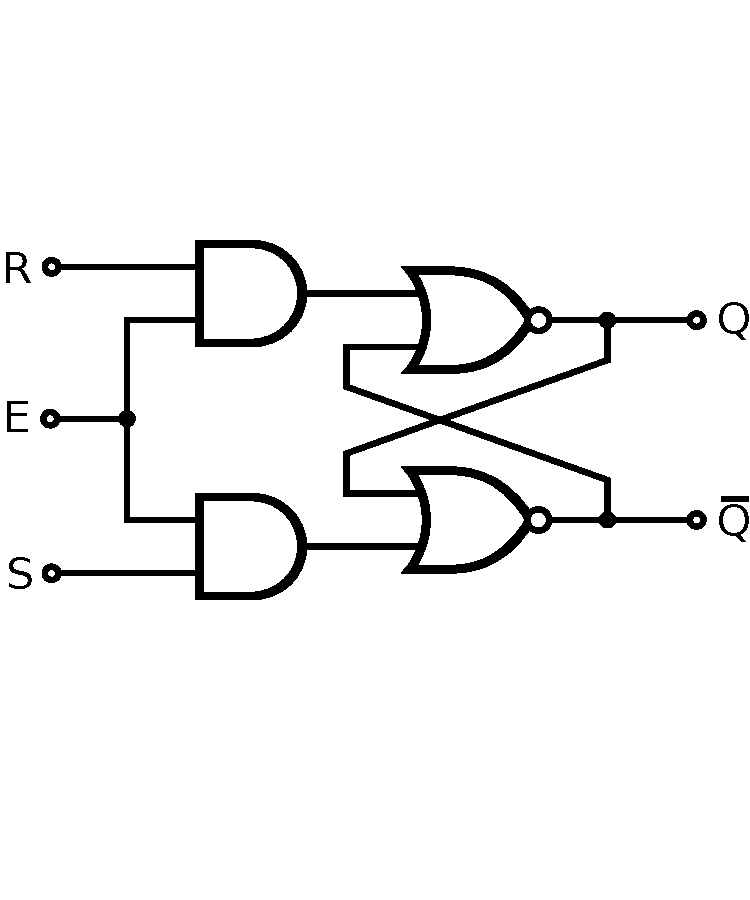
\includegraphics[width=10cm,height=4cm,keepaspectratio]{25.pdf}
\end{figure}
\Exercise
Using only two edge triggered D flip-flops design a circuit, which divides
the frequency of an input signal (clock) by 4. 
\begin{figure}[H]
  \centering
  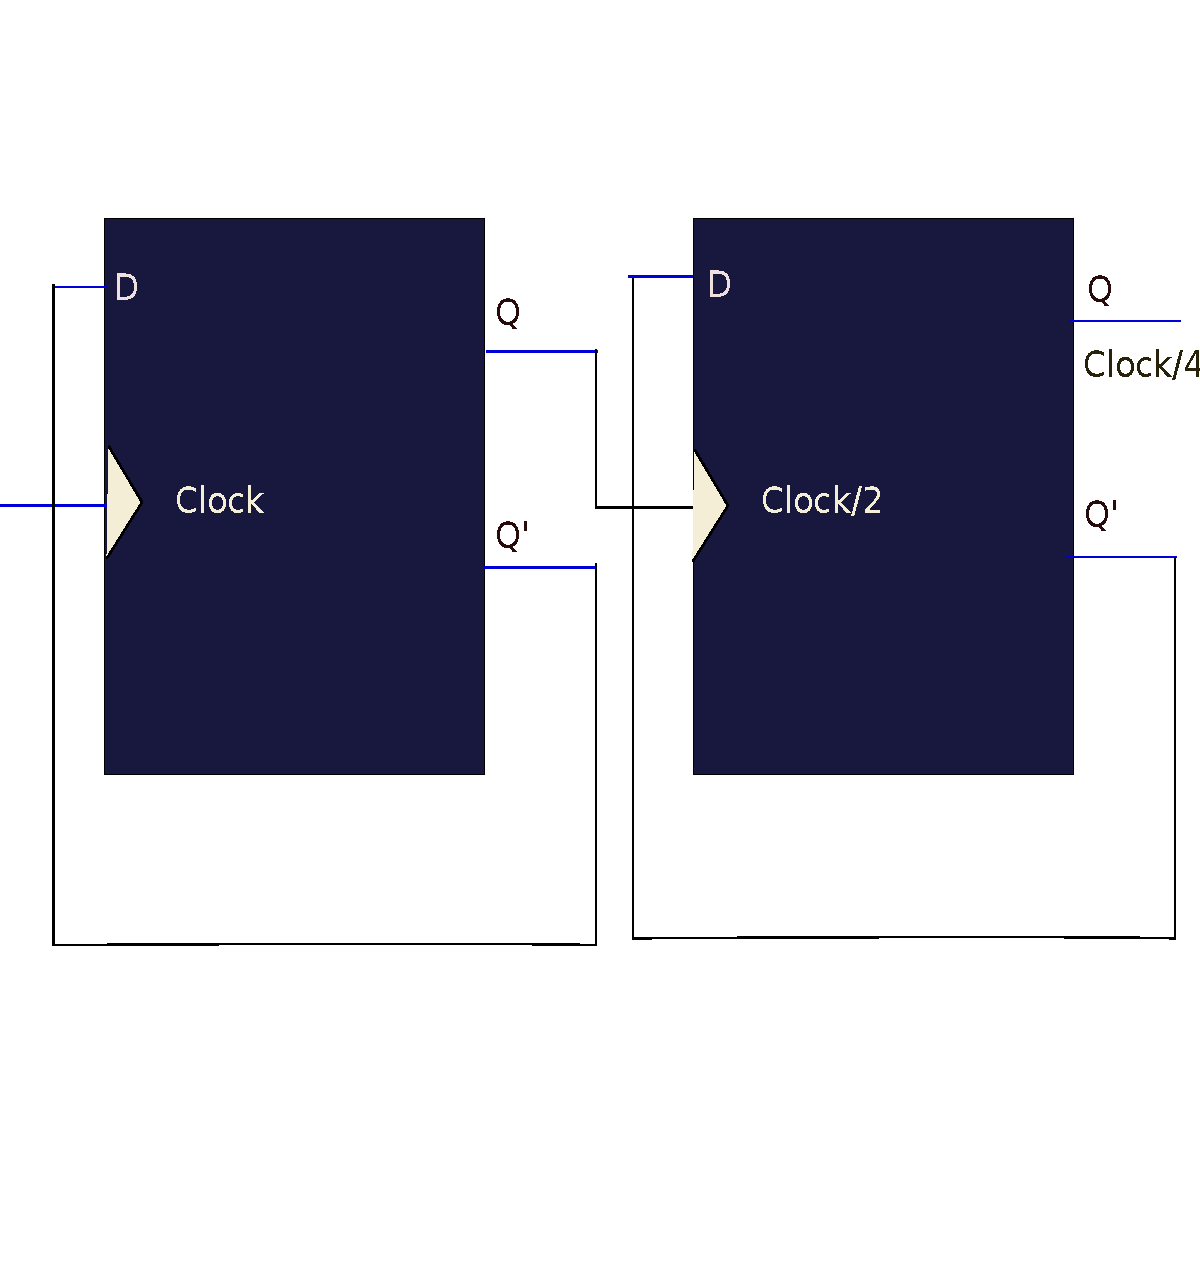
\includegraphics[width=10cm,height=8cm,keepaspectratio]{26.pdf}
  \caption{}
\end{figure}

\Exercise[difficulty=2]
Counters are essential components of any complex digital circuit. They are
essentially sequential circuits which loop through a specific set of states.
Design
a counter which generates 
a sequence of numbers (in binary form) from 0 to 7 and cycles back again to 0.
This is called a MOD 8 counter. 

\Answer
Any logic circuit with $n$ states can be made with at most $(\lceil \log_2 n \rceil)$ D flip-flops. So this circuit can be made using 
3 D flip-flops.\\

Let $D0$, $D1$, $D2$ and $Q0$, $Q1$, $Q2$ be the corresponding inputs and outputs of the 3 flip-flops.
$Qi_{now}$ is the present value of $Qi$ and $Qi_{next}$ is the next value of $Qi$ which is obtained by shorting $Qi_{now}$ with $Qi$ and  $Qi_{next}$ and $Di$. 
State table for the circuit:\\

\begin{tabular}{|c|c|c|c|c|c|}
\hline
$Q0_{now}$ & $Q1_{now}$ & $Q2_{now}$ & $Q0_{next}$ & $Q1_{next}$ & $Q2_{next}$ \\
\hline
0 & 0 & 0 & 0 & 0 & 1\\ 
\hline
0 & 0 & 1 & 0 & 1 & 0\\
\hline
0 & 1 & 0 & 0 & 1 & 1\\
\hline
0 & 1 & 1 & 1 & 0 & 0\\
\hline
1 & 0 & 0 & 1 & 0 & 1\\
\hline
1 & 0 & 1 & 1 & 1 & 0\\
\hline
1 & 1 & 0 & 1 & 1 & 1\\
\hline
1 & 1 & 1 & 0 & 0 & 0\\
\hline
\end{tabular} \\


Using K-maps, we simplify the logic function to obtain $Q_{next}$ (or $D$) in terms of $Q_{now}$ (or $Q$).\\
\\
$D0 = \overline {Q0}.Q1.Q2 + Q0.\overline{Q1}+Q0.\overline{Q2}\\
D1 = \overline{Q1}.Q2 + Q1.\overline{Q2}\\
D2 = \overline{Q2}$ \\
\\
This circuit can be implemented using simple logic gates. The output states are given by $Q0$ (MSB), $Q1$ and $Q2$ (LSB).
\Exercise[difficulty=2]
Using D flip-flops and logic gates, design a circuit, which generates the following sequence of numbers:
\[
001 \rightarrow 100 \rightarrow 010 \rightarrow 101 \rightarrow 110
\rightarrow 111 \rightarrow 011 \rightarrow 001 
\]

Assume that the circuit
never generates 000. This circuit can be used to generate pseudo-random numbers.

\Answer:
State table for the circuit:\\

\begin{tabular}{|c|c|c|c|c|c|}
\hline
$Q0$ & $Q1$ & $Q2$ & $D0$ & $D1$ & $D2$ \\
\hline
0 & 0 & 1 & 1 & 0 & 0\\ 
\hline
1 & 0 & 0 & 0 & 1 & 0\\
\hline
0 & 1 & 0 & 1 & 0 & 1\\
\hline
1 & 0 & 1 & 1 & 1 & 0\\
\hline
1 & 1 & 0 & 1 & 1 & 1\\
\hline
1 & 1 & 1 & 0 & 1 & 1\\
\hline
0 & 1 & 1 & 0 & 0 & 1\\
\hline
\end{tabular} \\

Here, \\
$D0 = Q1 \oplus Q2\\
D1 = Q0\\
D2 = Q1$\\


\end{ExerciseList}

\section*{Memories}

\begin{ExerciseList}

\Exercise
Compare the power, area and time of a SRAM, DRAM, and latch.

\Answer:\\
\begin{tabular}{||l|p{3cm}|p{3cm}|p{3cm}||}
\hline
\hline
 & Power & Area & Time per Access \\
\hline
SRAM & Medium  & Medium  &  Medium\\
\hline
DRAM & Low & Low & High \\
\hline
Latch & High & High & Low \\
\hline
\hline
\end{tabular}

\Exercise
Propose a design for the column mux/demux circuit.

\Exercise
What is the role of the {\em match} line in a CAM array?
\Answer
The {\em match} line is used to check if there is a match between the value stored in the CAM array and the input bit. A CAM array is addressed by its content, and we need to index each row by its content and be able to find out if there is a match between the content of the CAM cells and the input address bits or not. Hence, the {\em match} line is required. \\
Let V be the value stored in the CAM cell, and $A_i$ be the value of the input bit. If V=$\overline A_i$ , then by the transistor logic, the match line will be pulled to a logical 0 by one pair of the pass transistors. This indicates a mismatch between the input bit and the content of the CAM cell. However, if V= $A_i$, then the match line will be equal to a logical 1, indicating a match. \\
We can compare each row of the CAM cell with the input, A. If any row matches the input, the corresponding match line will have a value of 1. We can compute a logical OR of all the match lines, and decide if we can have a match in a CAM array or not. Also, all the match lines of the CAM array could be connected to a priority encoder to find the index of the row that matches the data. \\
\Exercise
What is the role of the {\em refresh logic} in a DRAM array?
\Answer
Suppose the capacitor in a DRAM cell is charged to a voltage equal to the supply voltage. In practice, the capacitor will gradually leak some charge though the dielectric, and the transistor. This current, though small, can be significant for a longer duration due to loss of charge, and ultimately discharge the capacitor. To prevent this, we need a {\em refresh logic}, or {\em refresh circuitry} to periodically refresh the value of a DRAM cell. We need to read the value and write it back. This needs to be done after a read operation as well because the capacitor loses some charge while charging the bit line. \\ 
\Exercise
Describe the design of a ROM and PROM cell.
\Answer
1. \textit{ROM cell} : \\
The structure of a ROM cell is similar to that of a DRAM cell. The capacitor in a DRAM cell stores a logical bit. If it stores a logical 1, then the charge across the capacitor is equal to the supply voltage $V_{dd}$, and if it stores a logical 0, then the charge across the capacitor is 0 V. Instead of having a capacitor, we can directly connect one end of the transistor to either ground or $V_{dd}$ depending on the bit that we wish to store. This is done at the time of manufacturing a chip. Hence, a ROM cell replaces the capacitor by a direct connection to $V_{dd}$ or ground. \\ \\
2. \textit{PROM cell} : \\
A PROM cell can be programmed once to store either a logical 1 or 0. Here, the connection between the transistor and ground is through an element called \textit{antifuse}. It is a weak conductor. When we transfer a large amount of current through the antifuse, it forms a conducting path, and drives the bit line to a logical 0. In this case, the cell stores a logical 0. Normally, when it does not form any conducting path, it does not have the ability to drive the bit line to a logical 0, and hence we infer that the cell stores a logical 1. Each bit line is precharged. After enabling the word line, if the voltage at the sense amplifiers does not increase then we can infer a logical 1. However, if the voltage keeps decreasing towards 0 V, then we can infer a logical 0. \\ 
\Exercise
Design a single PLA array to compute al the following Boolean functions:

\begin{enumerate}[a)]
\item  $A.B + B.C + C.A$
\item  $A.\overline{B}.\overline{C} + \overline{A}.B.C$
\item  $\overline{A+B}$
\end{enumerate}
\Answer
\begin{figure}[H]
  \centering
  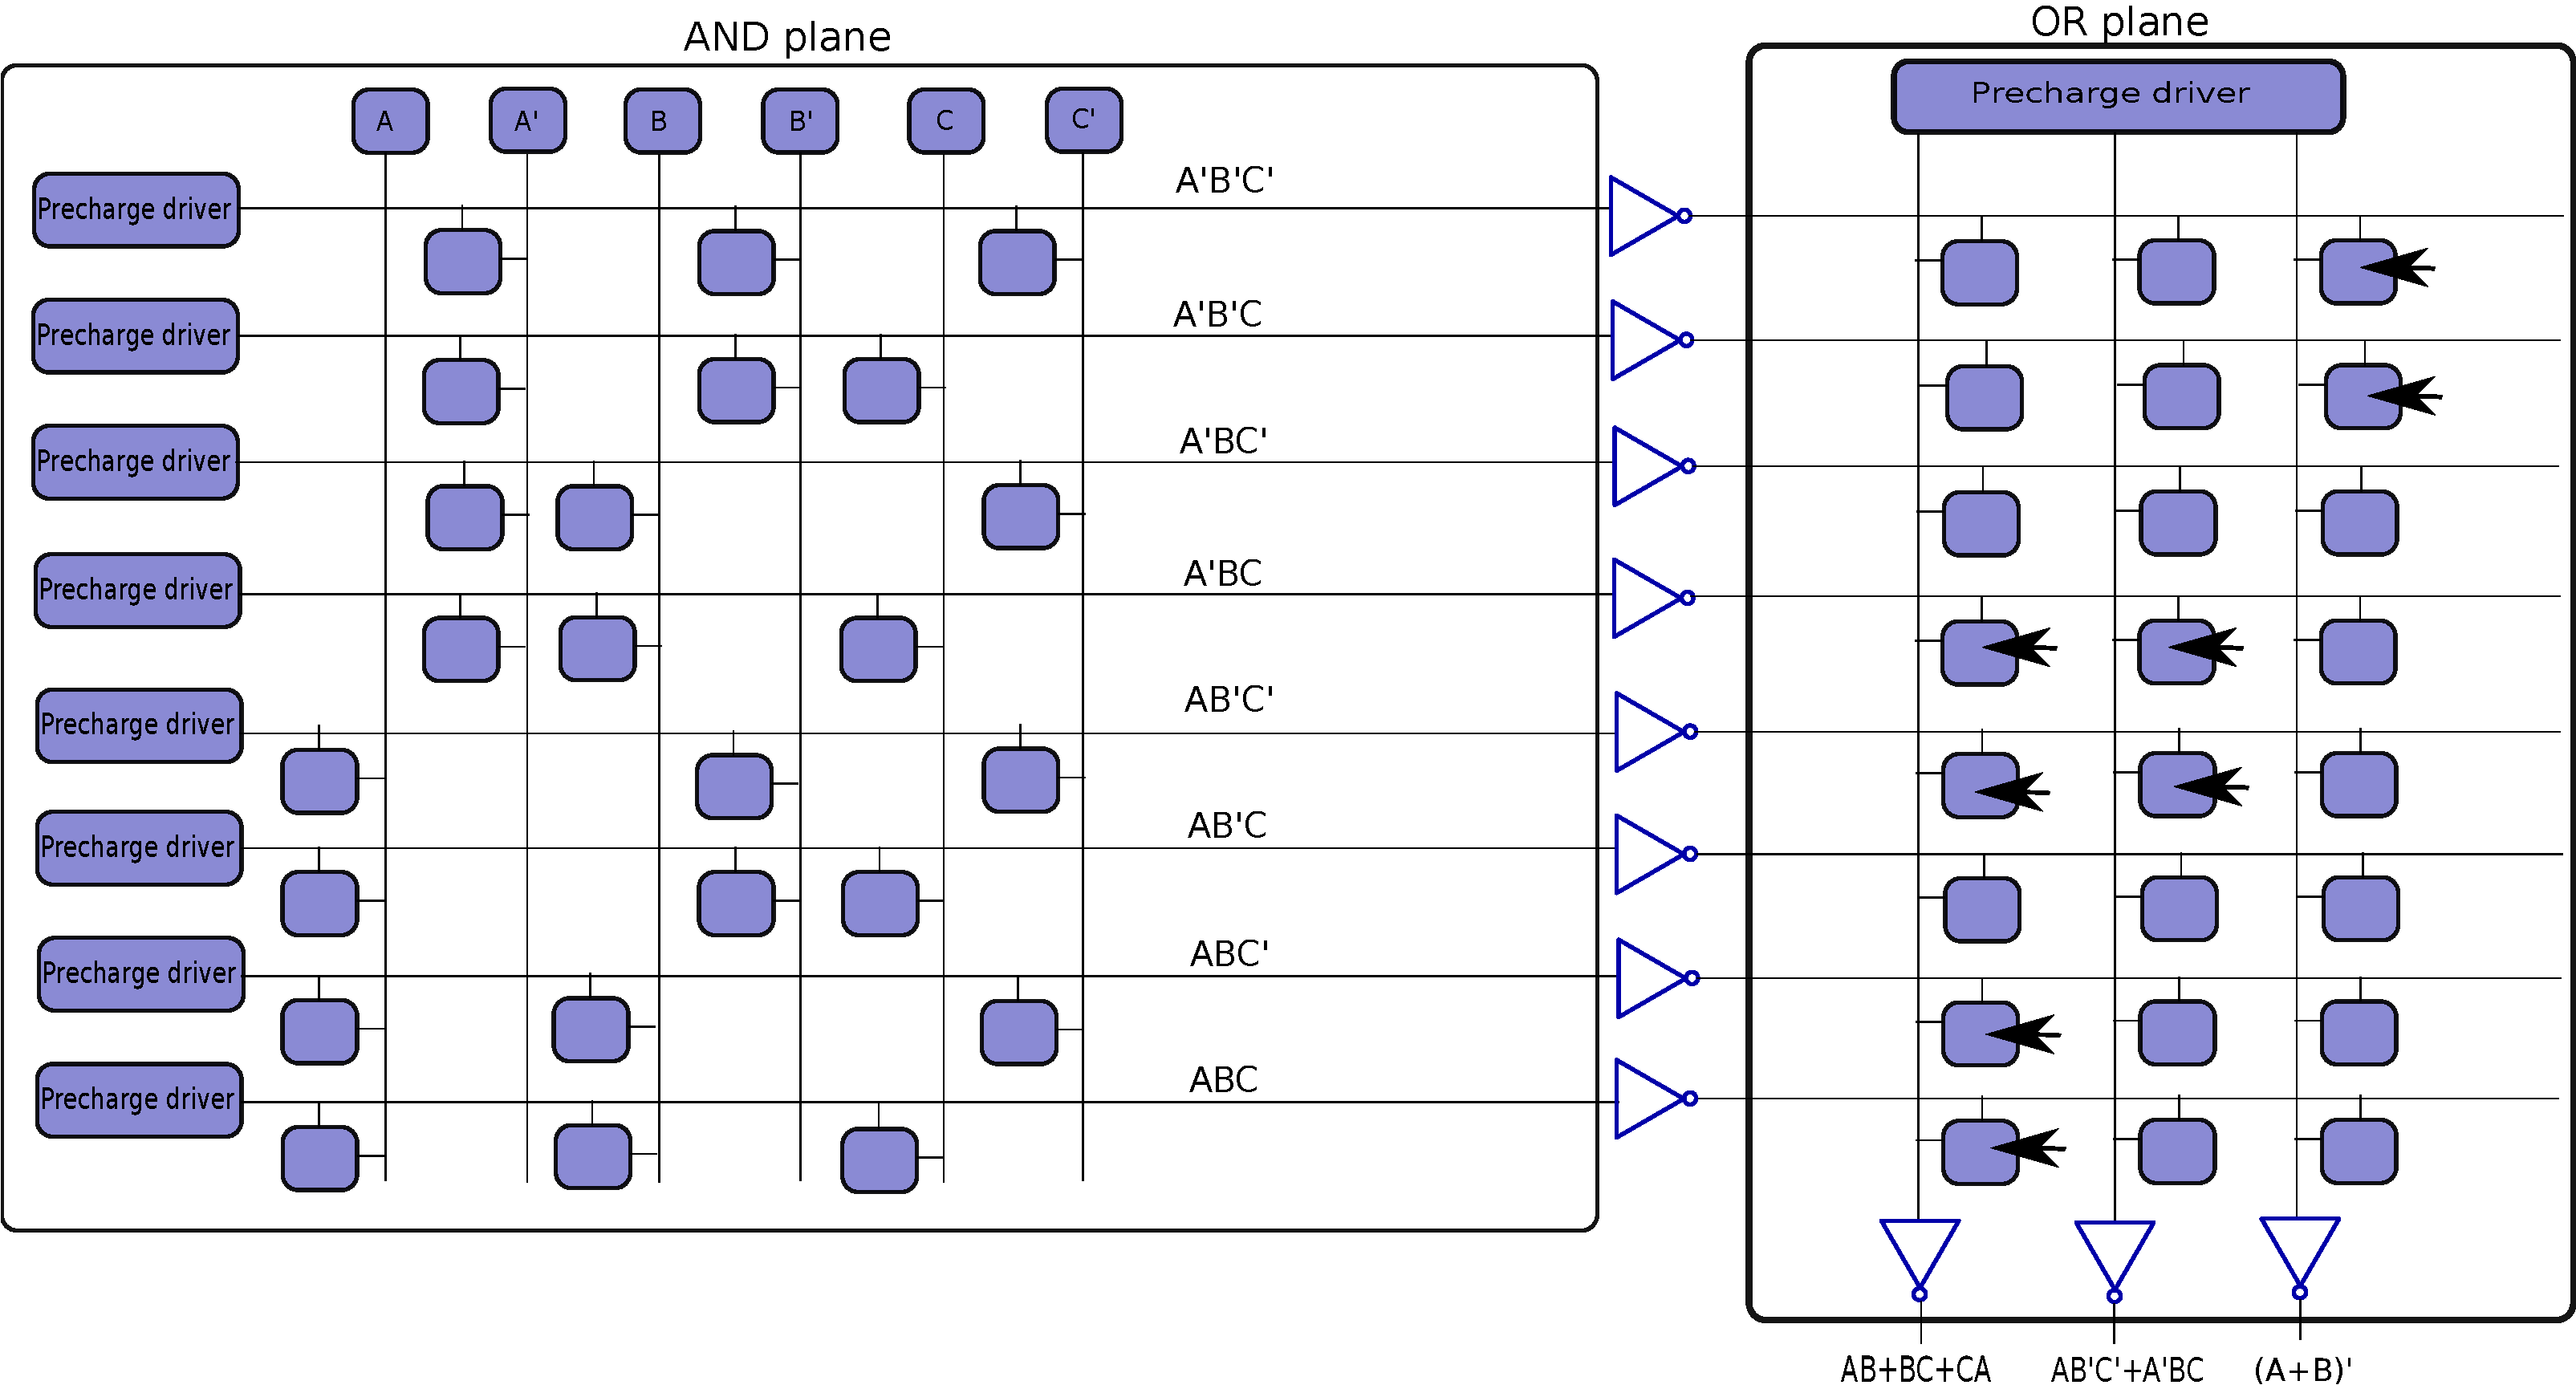
\includegraphics[width=17cm,height=30cm,keepaspectratio]{PLA.pdf}
  \caption{}
\end{figure}
\end{ExerciseList}

\section*{Design Problems}

\begin{ExerciseList}
\Exercise
Design the following circuits using a circuit simulator such as Spice and verify their operation:

\begin{enumerate}[a)]
\item NOT gate
\item NAND gate
\item D flip-flop
\item SRAM cell
\end{enumerate}

\Exercise
Prepare a report on novel memory technologies such as phase change memory, Ferro-electric
RAM, and magneto-resistive RAM. 
\end{ExerciseList}


\newpage
\chapter{Computer Arithmetic}
\vskip 2cm

\section*{Exercises}
\vskip 1cm

\setcounter{Exercise}{0}
\setcounter{Answer}{0}

\subsection*{Addition}

\begin{ExerciseList}

\Exercise
Design a circuit to find the 1's complement of a number using half adders only. 

\Exercise
Design a circuit to find the 2's complement of a number using half adders and logic gates. 

\Exercise
Assume that the latency of a full adder is 2ns, and that of a half adder is 1ns. What is the latency
of a 32 bit ripple carry adder?

\Exercise[difficulty=1]
Design a carry-select adder to add two n-bit numbers in $O(\sqrt{n})$ time, where
the sizes of the blocks are $1, 2, ... ,m$ respectively.

\Exercise
Explain the operation of a carry lookahead adder.

\Exercise[difficulty=1]
Suppose there is an architecture which supports numbers in base 3 instead of base 2. Design a Carry Lookahead Adder for
this system. Assume that you have a simple full-adder which adds numbers in base 3. 

\Answer
The following cases generate a carry:


\begin{enumerate}
	\item $1+2 = 10$
	\item $2+1 = 10$
	\item $2+2 = 11$
\end{enumerate}

$G_i = 1$ if it falls in the above 3 cases, otherwise $G_i = 0$. \\
The following case propagates a carry:
 
\begin{enumerate}
	\item $1+1 = 2$
\end{enumerate}

$P_i = 1$ for the only above case, otherwise $P_i = 0$.\\
The remaining things remain same as before.\\
$P_{ij} = P_{ik}\; .\; P_{kj}$ \hspace{24 mm} $i<k<j$\\
$G_{ij} = G_{kj}\;+\;(P_{kj}\;.\;G_{ik})$\hspace{10 mm} $i<k<j$\\ \\
No changes are required for Ripple Carry Adder and Carry Select Adder.



\Exercise[difficulty=1]
Most of the time, a carry does not propagate till the end.
In such cases, the correct output is available much before the worst case delay.
Modify a ripple carry adder to consider such cases and set an output line to high as soon as
the correct output is available.

\Answer
Defining Cumulative Carry Generate function $CG_i$ for every $i$ in Range 0 to 31:\\
$CG_i=G_{31}\;+\;G_{30}\;+\;......\;+\;G_i$\\
where $G_i$ is the Generate function corresponding to position $i$ in Carry Lookahead Adder.\\ The adder first computes
all these $CG_i$ (in constant amount of time). Then as soon as a carry $C_i$ is generated for position i, the adder
computes $(CG_{i+1}\; and \;C_i)$. If it is zero, it implies that there will be no carry propagation and generation any
further and the output from the adder is correct now. So adder can set an output line high indicating that it has
completed the addition.


\Exercise[difficulty=1]
Design an optimal adder, which uses only the propagate function, and simple
logic operations. It should NOT use the generate function. What is its time and space complexity?

\Answer
Let there be a block (i,j). Carry out of this block $C_{i,j}$:\\
$C_{i,j} = P_{i,j}$ + Carry generated in the block,\\
where $P_{i,j}$ is the propagate function for block (i,j).\\
We will use an alternative approach to get the carry generated in the block. First of all we divide the number in
$\sqrt{n}$ blocks, each of size $\sqrt{n}$. Now we can add the numbers is a block to get the carry out. This will take
O($\sqrt{n}$) amount of time. Calculating propagate functions will take O($\log n$) time. Now that we have the carry out
for each block, we can add the two complete numbers. Total time taken to add is O($\sqrt{n}$).

\Exercise
Design a hardware structure to compute the sum of $m$, $n$ bit numbers. Make it run as fast as possible. Show the design
of the structure. Compute a tight bound on its asymptotic time complexity. [NOTE: Computing the time
complexity is not as simple as it seems].


\Exercise[difficulty=2]
You are given a probabilistic adder, which adds two numbers and yields the output
ensuring that each bit is correct with probability, $a$.
In other words, a bit in the output may be wrong with probability, $(1-a)$, and this event is independent
of other bits being incorrect.
How will you add two numbers using using probabilistic adders 
ensuring that each output bit is correct with at least a probability of $b$, where $b>a$?


\Answer
A simple idea is to use multiple such adders in parallel. The bit at position $i$ of the final output should be the
result of majority function of the bits at position $i$ of the outputs produced by each adder. Suppose we use $n$ adders
in parallel (where $n$ is odd), then we have to find $n$ such that probability that at least $(n+1)/2$ bits are correct
$\geq b$. In other words, we have to find $n$ such that \\ \\ $\sum\limits_{r=(n+1)/2}^{n} \ a^{r}.(1-a)^{n-r} \geq b$
\\ \\
Solving the above equation, given the values of $a$ and $b$, we will have $n\geq k$, where $k$ is some constant. The
optimal number of adders is $ceil(k)$.

\Exercise[difficulty=3]
How frequently does the carry propagate to the end for most numbers? Answer: Very infrequently.
In most cases, the carry does not propagate beyond a couple of bits. Let us 
design an approximately correct adder. 
The insight is that a carry does not propagate by more than $k$ positions 
most of the time. Formally, we have: \\
{\bf Assumption 1:} While adding two numbers, the largest length of a chain of propagates
is at most $k$. \\

Design an optimal adder
in this case that has time complexity $O(log\, k)$ assuming that
Assumption 1 holds all the time. Now design a circuit to check if assumption 1
has ever been violated. Verma et. al.~\cite{brisk} proved that $k$ is equal to $O(log(n))$
with very high probability. Voila, we have an exactly correct adder,
which runs most of
the time in $O(log(log(n)))$ time.!!! \\


\Answer {\bf Circuit 1:}\\
Find out the generate function for each bit. Wherever generate function $G_i = 1$, select a chunk of $k$ bits starting
from there and compute the propagate functions for that chunk. Calculating generate function for all bits will take
$O(1)$ time and subsequent computation for propagate function will take $O(\log k)$ time. The complete structure is
similar to Carry Lookahead Adder except we do not need to compute generate and propagate functions for chunks larger
than k bits in size. Addition is done in the similar way.\\ {\bf Circuit 2:}\\
This circuit will check the carry-out from the chunks of k bits which were selected by circuit 1. If the carry-out from
each chunk is equal to 0, then there is no error. If the carry-out from any of the chunk becomes 1, then this circuit
reports an error and the addition is performed using different technique or by different adder.  

\Exercise[difficulty=3]
Let us consider two n bit binary numbers, $A$, and $B$. Further
assume that the probability of a bit being equal to 1 is $p$ in $A$, and $q$ in $B$. Let
us consider ($A + B$) as one large chunk(block).

(a) What are the expected values of generate and propagate functions of this
block as $n$ tends to $\infty$?

(b) If $p = q = \frac{1}{2}$,
 what are the values of these functions?
(c) What can we infer from the answer to part (b) regarding the fundamental
limits of binary addition?
\end{ExerciseList}

\section*{Multiplication}

\begin{ExerciseList}

\Exercise
\label{ex:mulexec}
Write a program  in assembly language (any variant) to multiply two unsigned 32-bit numbers given in
registers $r0$ and $r1$ 
and store the product in registers $r2$ (LSB) and $r3$ (MSB). Instead of using the multiply
instruction, simulate the algorithm
of the iterative multiplier. 

\Answer Code:
\begin{Verbatim}[frame=single]
L1:
	and r5, r3, #1
	cmp r5, #1
	addeq r2, r2, r0
	and r5, r2, #1
	mov r2, r2, lsr #1
	mov r3, r3, lsr #1
	cmp r5, #1
	addeq r3, r3, #0x80000000
	add r4, r4, #1
	cmp r4, #32
	bne L1
	mov pc, lr
multiply:
	mov r2, #0
	mov r3, r1
	mov r4, #0
	bl L1
\end{Verbatim}


\Exercise
Extend the solution to Exercise~\ref{ex:mulexec} for 32 bit signed integers.

\Answer
If a number is negative, take 2's compliment of it to make it positive. Do usual unsigned multiplication for the two
31-bit positive numbers to get the positive product. Calculate the sign of the product from the sign of the initial
multiplicand and initial multiplier : product is negative if and only if their signs are different. If the final product
is positive, leave it as it is, otherwise, take 2's compliment of the product.

\Exercise[difficulty=1]
Normally, in the Booth's algorithm, we consider the current bit, and the previous bit. Based on these two values, we
decide whether we need to add or subtract a shifted version of the multiplicand. This is known as the radix-2 Booth's
algorithm, because we are considering two bits at one time. There is a variation of Booth's algorithm, called radix-4
Booth's algorithm in which we consider 3 bits at a time. Show how this algorithm is faster than the original radix-2
Booth's algorithm. How will you implement this algorithm ?

\Answer
In this algorithm, we consider 3 bits at a time in a block, each block overlaps the previous block by 1 bit. We start
making groups from LSB and proceed towards MSB. Thus, by doing this, we essentially halve the number of groups formed;
since each alternate bit is now covered by only 1 group, while each bit (except for LSB and MSB) previously (in radix-2)
was covered by 2 groups. Following are the possibilities of the bit pattern in a group and corresponding product P.
Assume that the MSB of the group is at position i. Let M be the multiplicand.\\ 

\begin{tabular}{|l|c|}
\hline
Block & $P$ \\
\hline \hline
000 &	$P$ \\
\hline
001	& $P + 2^{i-1} * M$ \\
\hline
010	& $P + 2^{i-1} * M$ \\
\hline
011	& $P + 2^{i} * M$ \\
\hline
100	& $P - 2^{i} * M$ \\
\hline
101	& $P -2^{i-1} * M$\\
\hline
110	& $P -2^{i-1} * M$ \\
\hline
111	& $P$ \\
\hline
\end{tabular} \\

** Take care of boundary cases of LSB and MSB

\Exercise[difficulty=1]
Assume that in the sizes of the $U$ and $V$ registers are 32 bits in a 32 bit Booth multiplier. Is it possible to have an
overflow? Answer the question with an example. [HINT: Can we have an overflow in the first iteration itself?]

\Exercise[difficulty=1]
Prove the correctness of the Booth multiplier in your own words.

\Exercise
Explain the design of the Wallace tree multiplier. What is its asymptotic time complexity.

\Exercise[difficulty=2] Design a Wallace tree multiplier to multiply two signed 32 bit numbers, and save the result in a 32 bit
register. How do we detect overflows in this case?


\end{ExerciseList}

\section*{Division}

\begin{ExerciseList}

\Exercise Implementation of division using an assembly program.
\begin{enumerate}
\item[i) ] Write an assembly program for restoring division.
\item[ii) ] Write an assembly program for non-restoring division.
\end{enumerate}

\Answer Restoring division:
\begin{Verbatim}[frame=single]
L1:
	and r3, r8, #0x80000000
	mov r8, r8, lsl #1
	mov r7, r7, lsl #1
	cmp r3, #0
	addne r7, r7, #1
	cmp r7, r1
	subge r7, r7, r1
	addge r8, r8, #1
	add r4, r4, #1
	cmp r4, #32
	bne L1
	mov pc, lr
divideRestore:
	mov r8, r0
	mov r4, #0
	bl L1
\end{Verbatim}


Non-restoring division:
\begin{Verbatim}[frame=single]
L1:
	and r3, r8, #0x80000000
	mov r8, r8, lsl #1
	mov r7, r7, lsl #1
	cmp r3, #0
	addne r7, r7, #1
	cmp r7, #0
	subge r7, r7, r1
	addlt r7, r7, r1
	cmp r7, #0
	addge r8, r8, #1
	add r4, r4, #1
	cmp r4, #32
	bne L1
	cmp r7, #0
	addlt r7, r7, r1
	mov pc, lr
divideNonRestore:
	mov r8, r0
	mov r4, #0
	bl L1
\end{Verbatim}

\Exercise[difficulty=1]
Design an $O(log(n)^k)$ time algorithm to find out if a number is divisible by 3. Try to minimise $k$. 

\Answer
If a number is divisible by 3, the absolute value of difference of the sum of bits at odd position and even positions is 
divisible by 3. \\
That is:\\
A number n is divisible by 3 iff:\\
$(\sum b_{2k+1} - \sum b_{2k})$ MOD $3 =0$\\
where $b_i$ is a bit of n at position i.\\
or,\\
$((b_1-b_0) + (b_3-b_2) + (b_5-b_4) + (b_7-b_6) .... )$ MOD 3 $= 0$\\
$\Rightarrow (((b_1-b_0)$ MOD 3 $+ (b_3-b_2)$ MOD 3$)$ MOD 3 $+ ((b_5-b_4)$ MOD 3 $+ (b_7-b_6)$ MOD 3$)$ MOD 3 $.... )$ MOD 3 $= 0 $\\ ...and so on.
So essentially, we build a circuit which calculates $(b_{2k+1} - b_{2k})$ MOD 3 in the first step, and then combines the
result by adding the subsequent pairs modulo 3, until a final result is obtained. If this final result in 0, the number
is divisible by 3.\\
The following figure shows an example of an 8 bit number $(11100111)_2$ through our circuit:\\

\begin{center}
%\includegraphics[bb=0 0 200 350,scale=0.5]{div3.png}
\end{center}

Total number of levels in the circuit = $log_2(n)$\\
Therefore, $k=1$;

\Exercise[difficulty=1]
Design an $O(log(n)^k)$ time algorithm to find out if a number is divisible by 5. Try to minimise $k$. 

\Exercise[difficulty=2]
Design a fast algorithm to compute the remainder of the division of an unsigned number
by a number of the form ($2^m + 1$). What is its asymptotic time complexity?

\Exercise[difficulty=2]
Design a fast algorithm to compute the remainder of the division of an unsigned number
by a number of the form ($2^m - 1$). What is its asymptotic time complexity?

\Exercise[difficulty=2]
Design an $O((log(uv))^2)$ algorithm to find the greatest common divisor of two binary numbers $u$ and $v$.
[HINT: The gcd of two even numbers $u$ and $v$ is $2*gcd(u/2,v/2)$]
\Answer
The algorithm, also known as Stein's algorithm is as follows:

\begin{enumerate}
	\item[1. ] $gcd (v, v) = v$
	\item[2. ] $gcd(0, v) = v$, and $gcd(u, 0) = u$ 
	\item[3. ] If $u$ and $v$ are both even, then $gcd(u, v) = 2\:.\:gcd(u/2, v/2)$
	\item[4. ] If $u$ is even and $v$ is odd, then $gcd(u, v) = gcd(u/2, v)$, because $2$ is not a common divisor. Similarly for the other case, then $gcd(u, v) = gcd(u, v/2)$.
	\item[5. ] If $u$ and $v$ are both odd:
	\begin{enumerate}
		\item[i) ] If $u \geq v$, then $gcd(u, v) = gcd((u - v)/2, v)$ 
		\item[ii) ] If $u < v$, then $gcd(u, v) = gcd((v - u)/2, u)$
	\end{enumerate}
\end{enumerate}
Each step reduces at least one of the operand by at least a factor of two.  Thus, this algorithm runs in
$O((log(uv))^2)$ in worst case. Or in other words, this algorithm takes time proportional to square of number of bits in
$u$ and $v$ together. 


\end{ExerciseList}

\section*{Floating Point Arithmetic}

\begin{ExerciseList}

\Exercise
Give the simplest possible algorithm to compare two 32 bit IEEE 754 floating point numbers. Do not consider $\pm
\infty$, NAN, and (negative 0).  Prove that your algorithm is correct. What is its time complexity ?

\Answer
Just compare the numbers like integers. IEEE 754 floating point numbers have their 1st bit as sign bit (which is same as
integers), next 8 bits store the exponent and the last 23 bits store mantissa. When we compare two fractions, we first
check the sign, then the exponent and finally the mantissa. If the signs are different, the comparison is done and the
positive one is greater (which is done correctly by comparing them as normal integers). If the two fractions are
positive, the one with greater exponent will be greater. This again will be done correctly by normal integer comparison
as exponent is placed to the left of mantissa. If the two fractions are negative, the one with greater exponent is
smaller, again done correctly by integer comparison: negative integer with higher first 8 bits after MSB is smaller.
Then comes the mantissa which is also checked correctly by integer comparison. \\ Time complexity = O(log n) taken for
subtraction and sign comparison, where n is the number of bits.



\Exercise 
Design a circuit to compute $\lceil log_2(n) \rceil$. What is its asymptotic time complexity?

\Exercise $A$ and $B$, are saved in the computer as $A'$ and $B'$. Neglecting any further truncation or roundoff errors, show that the relative error of the product is approximately the sum of the relative errors of the factors.  \Answer Let $\alpha$ be the relative error in $A'$ and $\beta$ be the relative error in $B'$. \\ So, $|\alpha| < 1$ and $|\beta| < 1$ \\ $A=A' * (1+\alpha) \\ B=B' * (1+\beta) \\ A*B = A'B' * ( 1+ \alpha + \beta + \alpha\beta) \\ = A'B' * (1+\alpha+\beta)(1+\alpha\beta/(1+\alpha+\beta)) \\ $
Since $\alpha$ and $\beta$ are small quantities with absolute value less than 1, $\alpha\beta / (1+\alpha+\beta) \longrightarrow 0$\\
Therefore, \\
$A*B \approx A'B' * (1+ (\alpha+\beta))\\
		= A'B' *(1+\delta) $\\
where $\delta = \alpha + \beta$

\Exercise
Show the flowchart for floating point addition.

\Exercise
Show the flowchart for floating point multiplication.

\Exercise
Can we use regular floating point division for dividing integers also? If not, then how can we modify the algorithm
for performing integer division? 

\Exercise
Describe in detail how the ``round to nearest'' rounding mode is implemented.

\Exercise[difficulty=3]
We wish to compute the square root of a floating point number in hardware using the Newton-Raphson method.
Outline the details of an algorithm, prove it, and compute its computational complexity.
Follow the following sequence of steps. 

\begin{enumerate}
\item Find an appropriate objective function. 
\item Find the equation of the tangent, and the point at which it intersects the x-axis. 
\item Find an error function. 
\item Calculate an appropriate initial guess for $x$. 
\item Prove that the magnitude of the error is less than 1.
\item Prove that the error decreases at least by a constant factor per iteration. 
\item Evaluate the asymptotic complexity of the algorithm. 
\end{enumerate} 

\Answer 
\begin{enumerate}
\item Objective function: $f(x) = x^2 - b$
Assume that $1/2 \le b < 2$. Any floating point number in the normal form can be brought to this form by
rounding the exponent to the nearest even number. Example. $1.5 \times 2^{-3} = 0.75 \times 2^{-2}$. 
\item Slope = 2x. Point at which the tangent intersects the x-axis ($x_2$):
\begin{equation}
\begin{split}
\frac{x_1^2 - b}{x_1 - x_2} = 2x_1 \\
\Rightarrow x_2 = \frac{x_1^2 + b}{2x_1} 
\end{split}
\end{equation}
\item Error function:  $E(x)  = x - \sqrt{b}$
\begin{equation}
\begin{split}
E(x_2) & = x_2 - \sqrt{b} \\
       & = \frac{x_1^2 + b}{2x_1} - \sqrt{b} \\
       & = \frac{x_1^2 + b - 2x_1\sqrt{b}}{2x_1} \\
       & = \frac{(x_1 - \sqrt{b})^2}{2x_1} \\
       & = \frac{E(x_1)^2}{2x_1}
\end{split}
\end{equation}
\item Initial guess for $x$: x = 1

\item Initial value of the error: $1 - \sqrt{b}$. 
\[
(1/2 \le b < 2) \Rightarrow (1 - \sqrt{2}) < (1 - \sqrt{b}) \le (1 - 1/\sqrt{2}) 
\]
Hence, $\mid 1 - \sqrt{b} \mid < 1$
\item 
Let us prove by induction that $x_n \ge 1/2$, and $b \ge x_n / 2$. 
This is true for the base case $x_1 = 1$. 

Assume the hypothesis is true for $x_n = x'$.
Let us try to prove that the hypothesis holds for $x_{n+1} = x''$.

\begin{equation}
\begin{split}
x'' & = \frac{x'^2 + b}{2x'} \\
   & = \frac{x'}{2} + \frac{b}{2x'} 
\end{split}
\end{equation}

Now, $x'/2 \ge 1/4$ (because, $x' \ge 1/2$), and $b/2x' \ge 1/4$ (because $b \ge x' / 2$).
Hence, $x'' \ge 1/2$.

Let us now prove that $b \ge x''/2$. We have:

\begin{equation}
\begin{split}
 & b \ge x''/2  \\
\Leftrightarrow & b \ge \frac{x'^2 + b}{4x'} \\
\Leftrightarrow & b \ge \frac{x'}{4} + \frac{b}{4x'} \\
\end{split}
\end{equation} 

By the induction hypothesis, $b/2 \ge x'/4$. 
If we prove that $b/2 \ge b/4x'$, we are done.

\begin{equation}
\begin{split}
& \frac{b}{2} \ge  \frac{b}{4x'} \\
\Leftrightarrow & 1 \ge \frac{1}{2x'} \\
\Leftrightarrow & x' \ge \frac{1}{2} (TRUE) \\ 
\end{split}
\end{equation}


We have thus proved the induction, and we can conclude that $x_n \ge 1/2$ for all values of $n$. 
Hence, $\forall n,2x_n \ge 1$.
We thus have: 
\[
E(x_{n+1}) \le E(x_n)^2 
\]

\item We have $log(n)$ steps because, we assume that the precision is till $n$ bits. In each step, 
we have to do a left shift and round (log(n)), addition (log(n)), and division ($log(n)^2$).

Thus, the total time complexity is \fbox{$O(log(n)^3)$}
\end{enumerate}

\noindent {\bf Note to TAs:} : (a and b) should have a reduced form of $b$  (1 mark) (c) 1 mark
(d and e) 1 mark (f) 4 marks (g) 1 mark. Take a look at part (f) carefully, it is the crux of the algorithm.
The proof should be crystal clear (for full marks). If there is any ambiguity, the benefit of doubt goes to the TA.
For this answer, we need to assume that the time complexity of a division is $O(log(n)^2)$ (This is a research
question). 

\end{ExerciseList}

\section*{Design Problems}
\begin{ExerciseList}

\Exercise
Implement an adder, multiplier, in a hardware description language such as VHDL or Verilog.

\Exercise
Extend your design for implementing floating point addition and multiplication.

\Exercise
Read about the SRT division algorithm, comment on its computational complexity, and try to implement it in
VHDL/Verilog.
\end{ExerciseList}












































\newpage
\chapter{Processor Design}
\begin{flushright}
\textbf{Solutions prepared by Prajwala TM $<$prajwala.tm@gmail.com$>$}
\end{flushright}
\section*{Exercises}
\vskip 1cm

\setcounter{Exercise}{0}
\setcounter{Answer}{0}

\section*{Hardwired Processor Design}

\begin{ExerciseList}

\Exercise
We have divided a \simplerisc processor into 5 distinct units. List them,
and describe their functions.

\Answer
The five stages of a SimpleRisc processor are :\newline

1. \hspace{4mm}Instruction Fetch:
The first step is to fetch instructions from memory. The fetch stage has logical elements to compute the address of the next instruction. If the current instruction is not a branch, then we need to add the size of the next current instruction to the address stored in the PC. If its a branch, then the address of the next instruction depends on the outcome and target of the branch. This information is obtained from the other units of the processor.\newline

2.\hspace{4mm} Instruction Decode:
This stage decodes the instruction and fetches the operands from registers. Dedicated logic circuits that generate signals based on the fields in the instruction are used for decoding.These signals are used by the other modules to process the instruction properly. \newline

3. \hspace{4mm}Execute:
This stage is used for performing arithmetic and logical operations.It makes use of the Arithmetic and Logical Unit (ALU) for the same. This part of the processor is used for obtaining the outcome of branches also, and is used for making a decision regarding the address of the next instruction.\newline

4.\hspace{4mm}Memory Access:
It contains the memory unit for processing load-store instructions and is used for interfacing with memory system. The values of the operands are fetched from and written to memory during this stage of execution of the instruction.\newline

5.\hspace{4mm} Register WriteBack :
In this stage, the results of the ALU or those obtained from the memory are written to the registers in the Register File. SimpleRisc assumes that we have 16 registers, out of which, the first 14 are general purpose, and can be used for any purpose. Register 14 is known as a stack pointer and Register 15 is used as a return address register.There are two special registers known as flags, which are not visible to the programmer.

\Exercise
Explain the terms -- {\em data path} and {\em control path}?

\Answer
There are two kinds of elements in a circuit. The first type of elements are registers,memories,arithmetic and logic circuits to process data values. The second type of elements are control units that decide the direction of the flow of data.\newline
Thus,the processor consists of two subsystems.\newline

The first subsystem is known as the \textit{datapath}.It consists of all the elements in a processor that are dedicated to storing, Sretrieving and processing data such as register files,memories, and ALUs.\newline

The second subsystem is known as the \textit{control path}. It primarily contains the control unit, whose role is to generate appropriate signals called control signals to control the movement of instructions, and data in the datapath.

\Exercise How does having a lesser number of instruction formats help in the process
of decoding an instruction?

\Answer
The number of instruction formats is one of the factors that affects the process of instruction decoding. Having a lesser number of instruction formats requires less circuitry which, in turn, implies less complexity of the intruction decoding unit. Less complexity leads to faster decoding, and hence, the processing speed of the instructions increases on the whole. 

\Exercise Draw the circuit for calculating the value of the 32 bit immediate, from
the first 18 bits of the instruction. Take the modifiers into account.

\begin{figure}[H]
  \centering
  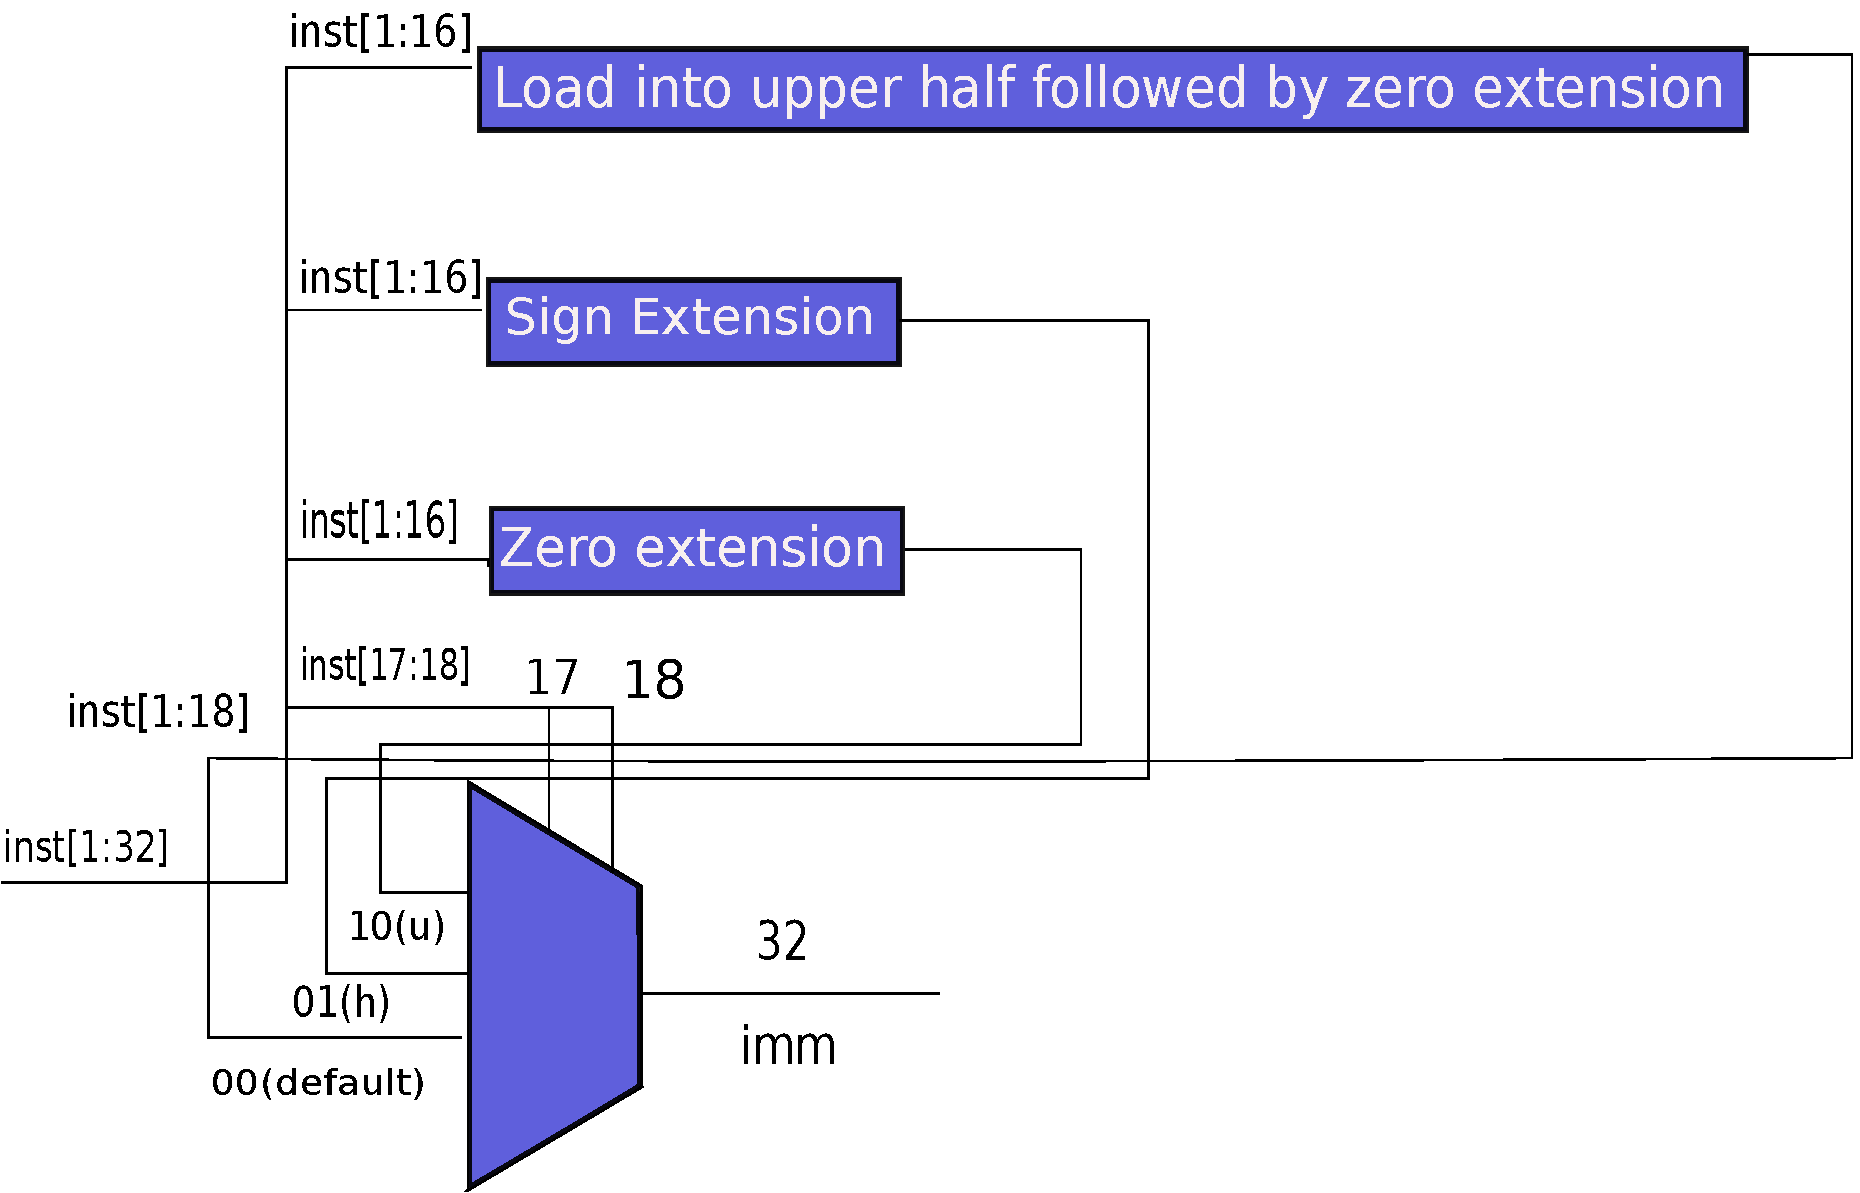
\includegraphics[width=10cm,height=8cm,keepaspectratio]{imm.pdf}
\end{figure}

\Exercise Why is it necessary for the register file in our \simplerisc processor
to have 2 read ports, and 1 write port?

\Answer
The \textit{SimpleRisc} instruction set has 21 instructions in its ISA. Looking at the list of instruction opcodes, it is clear that each instruction has atmost 2 read registers, and atmost 1 write back register. Hence, in the Instruction decode stage, it is necessary to have a Register file with 2 read ports and 1 write port for correct decoding.

\Exercise Why do we need 2 multiplexers in the OF stage of the processor? What are their
functions?

\Answer
The register file used in the decode(Operand Fetch) stage has 2 read ports and 1 write port. For the first register operand op1, we have two choices. For ALU,Memory instructions, we need to read the first source register,rs1. For \textit{ret},we need to read the value of the return register,\textit{ra}. In order to make a choice between the contents of the instruction fields \textit{rs1} or \textit{ra},we need to use a multiplexer. This is controlled by the control signal \textit{IsRet}. The output of the multiplexer is the input to the Register file's first read port, and is known as \textit{op1}.\newline
For instructions other than \textit{store}, the second source register is specified by \textit{rs2}. However, for the store instruction, we need to use the source register \textit{rd}. This choice between \textit{rs2} and \textit{rd} is made by using a second multiplexer. This is in turn, controlled by the \textit{isStore} signal. The output of the multiplexer is the input to the Register file's second read port and is known as \textit{op2}. \newline

\Exercise
Let us propose to compute the branch outcome and target in the OF stage. Describe the
design of the OF stage with this functionality.

\Answer
The operand fetch unit has two functions :1)calculate the values of the immediate operand and branch target 2)read the source registers\newline
The value of the immediate operand is calculated by extracting the \textit{imm} field from the instruction. The 32 bit value is calculated by extending the 18 bit \textit{imm} in accordance with the modifiers.\newline
The \textit{branchTarget} is calculated by first extracting the 27 bit offset, shifting by 2 bits and extending the sign. This is added to the PC to get the      \textit{branchTarget}.\newline
In case of the \textit{ret} instruction, the \textit{branchTarget} is the contents of the \textit{ra} register, read from the Register File. To choose between these two, a multiplexer is used, whose outcome is the required \textit{branchPC} value.\newline
The next part of the Fetch Unit is used to read the source registers and obtain the values of \textit{op1} and \textit{op2}. This is done with the help of the Register files, and the multiplexers.

\begin{figure}[H]
  \centering
  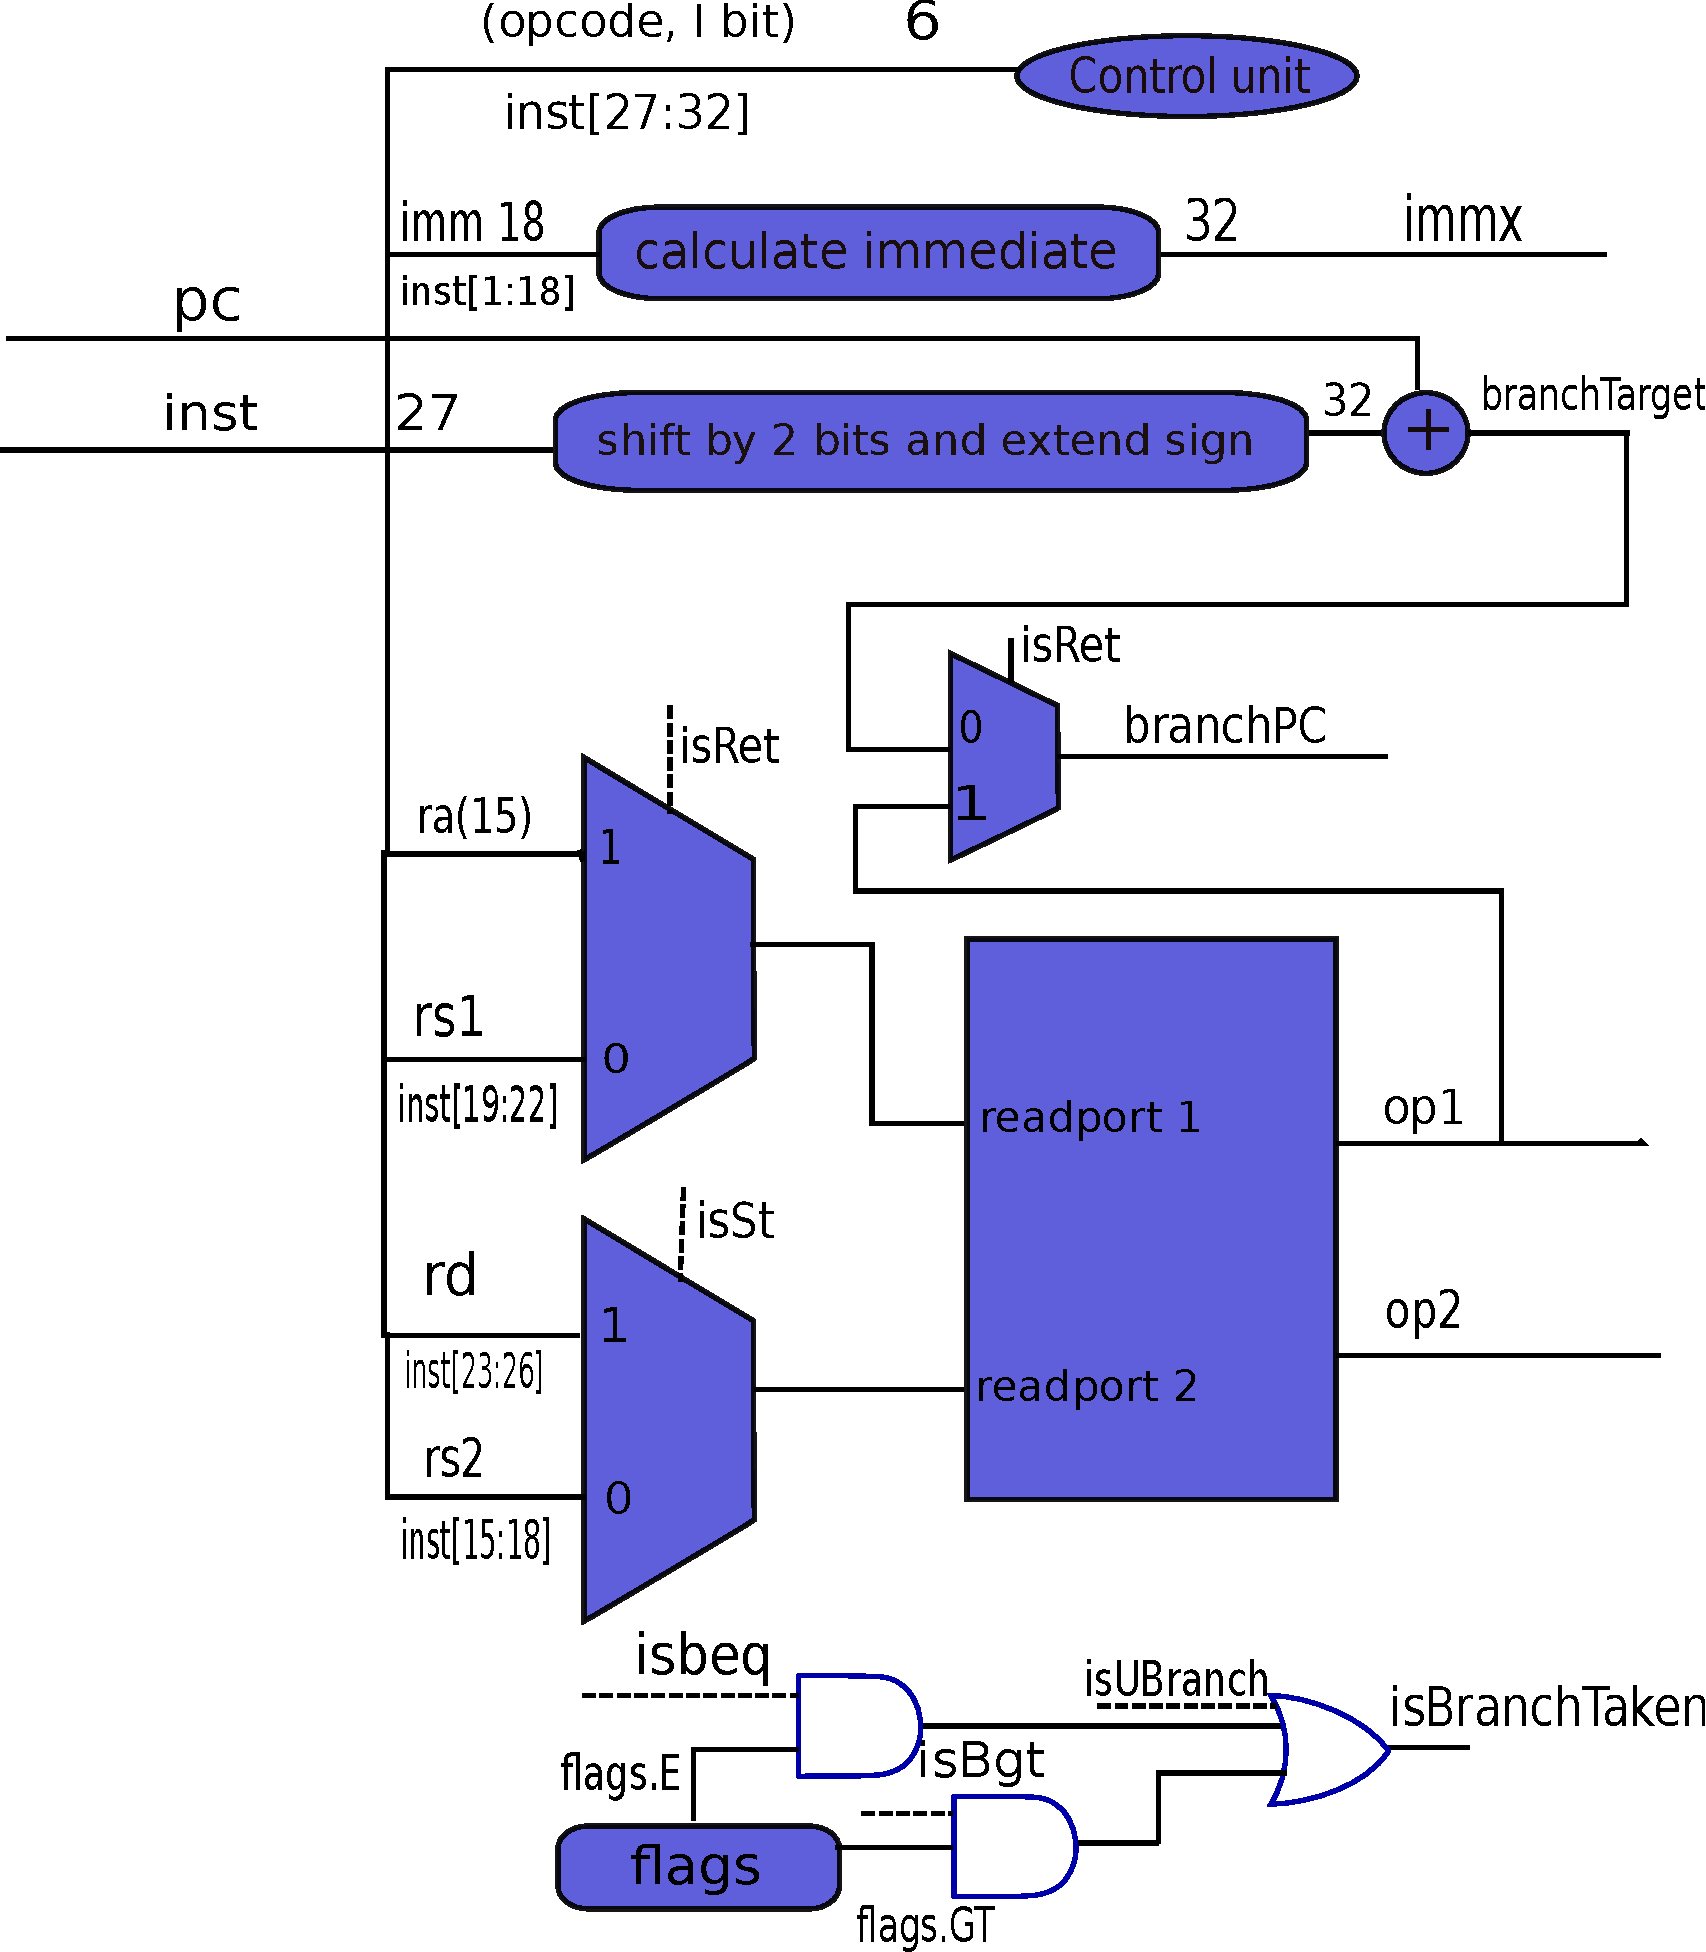
\includegraphics[width=10cm,height=10cm,keepaspectratio]{branch.pdf}
\end{figure}

\Exercise[difficulty=1]
For the ALU we use a multiplexer with a large number of inputs.
How can we implement this multiplexer
with transmission gates? (show a circuit diagram, and explain why your idea will
work) 
\Answer
\hspace{1mm} \\
The multiplexer can be implemented using tranmission gates. We use three select lines $S0$,$S1$,$S2$ to choose one of the outputs of the different modules of the ALU.
\begin{figure}[H]
  \centering
  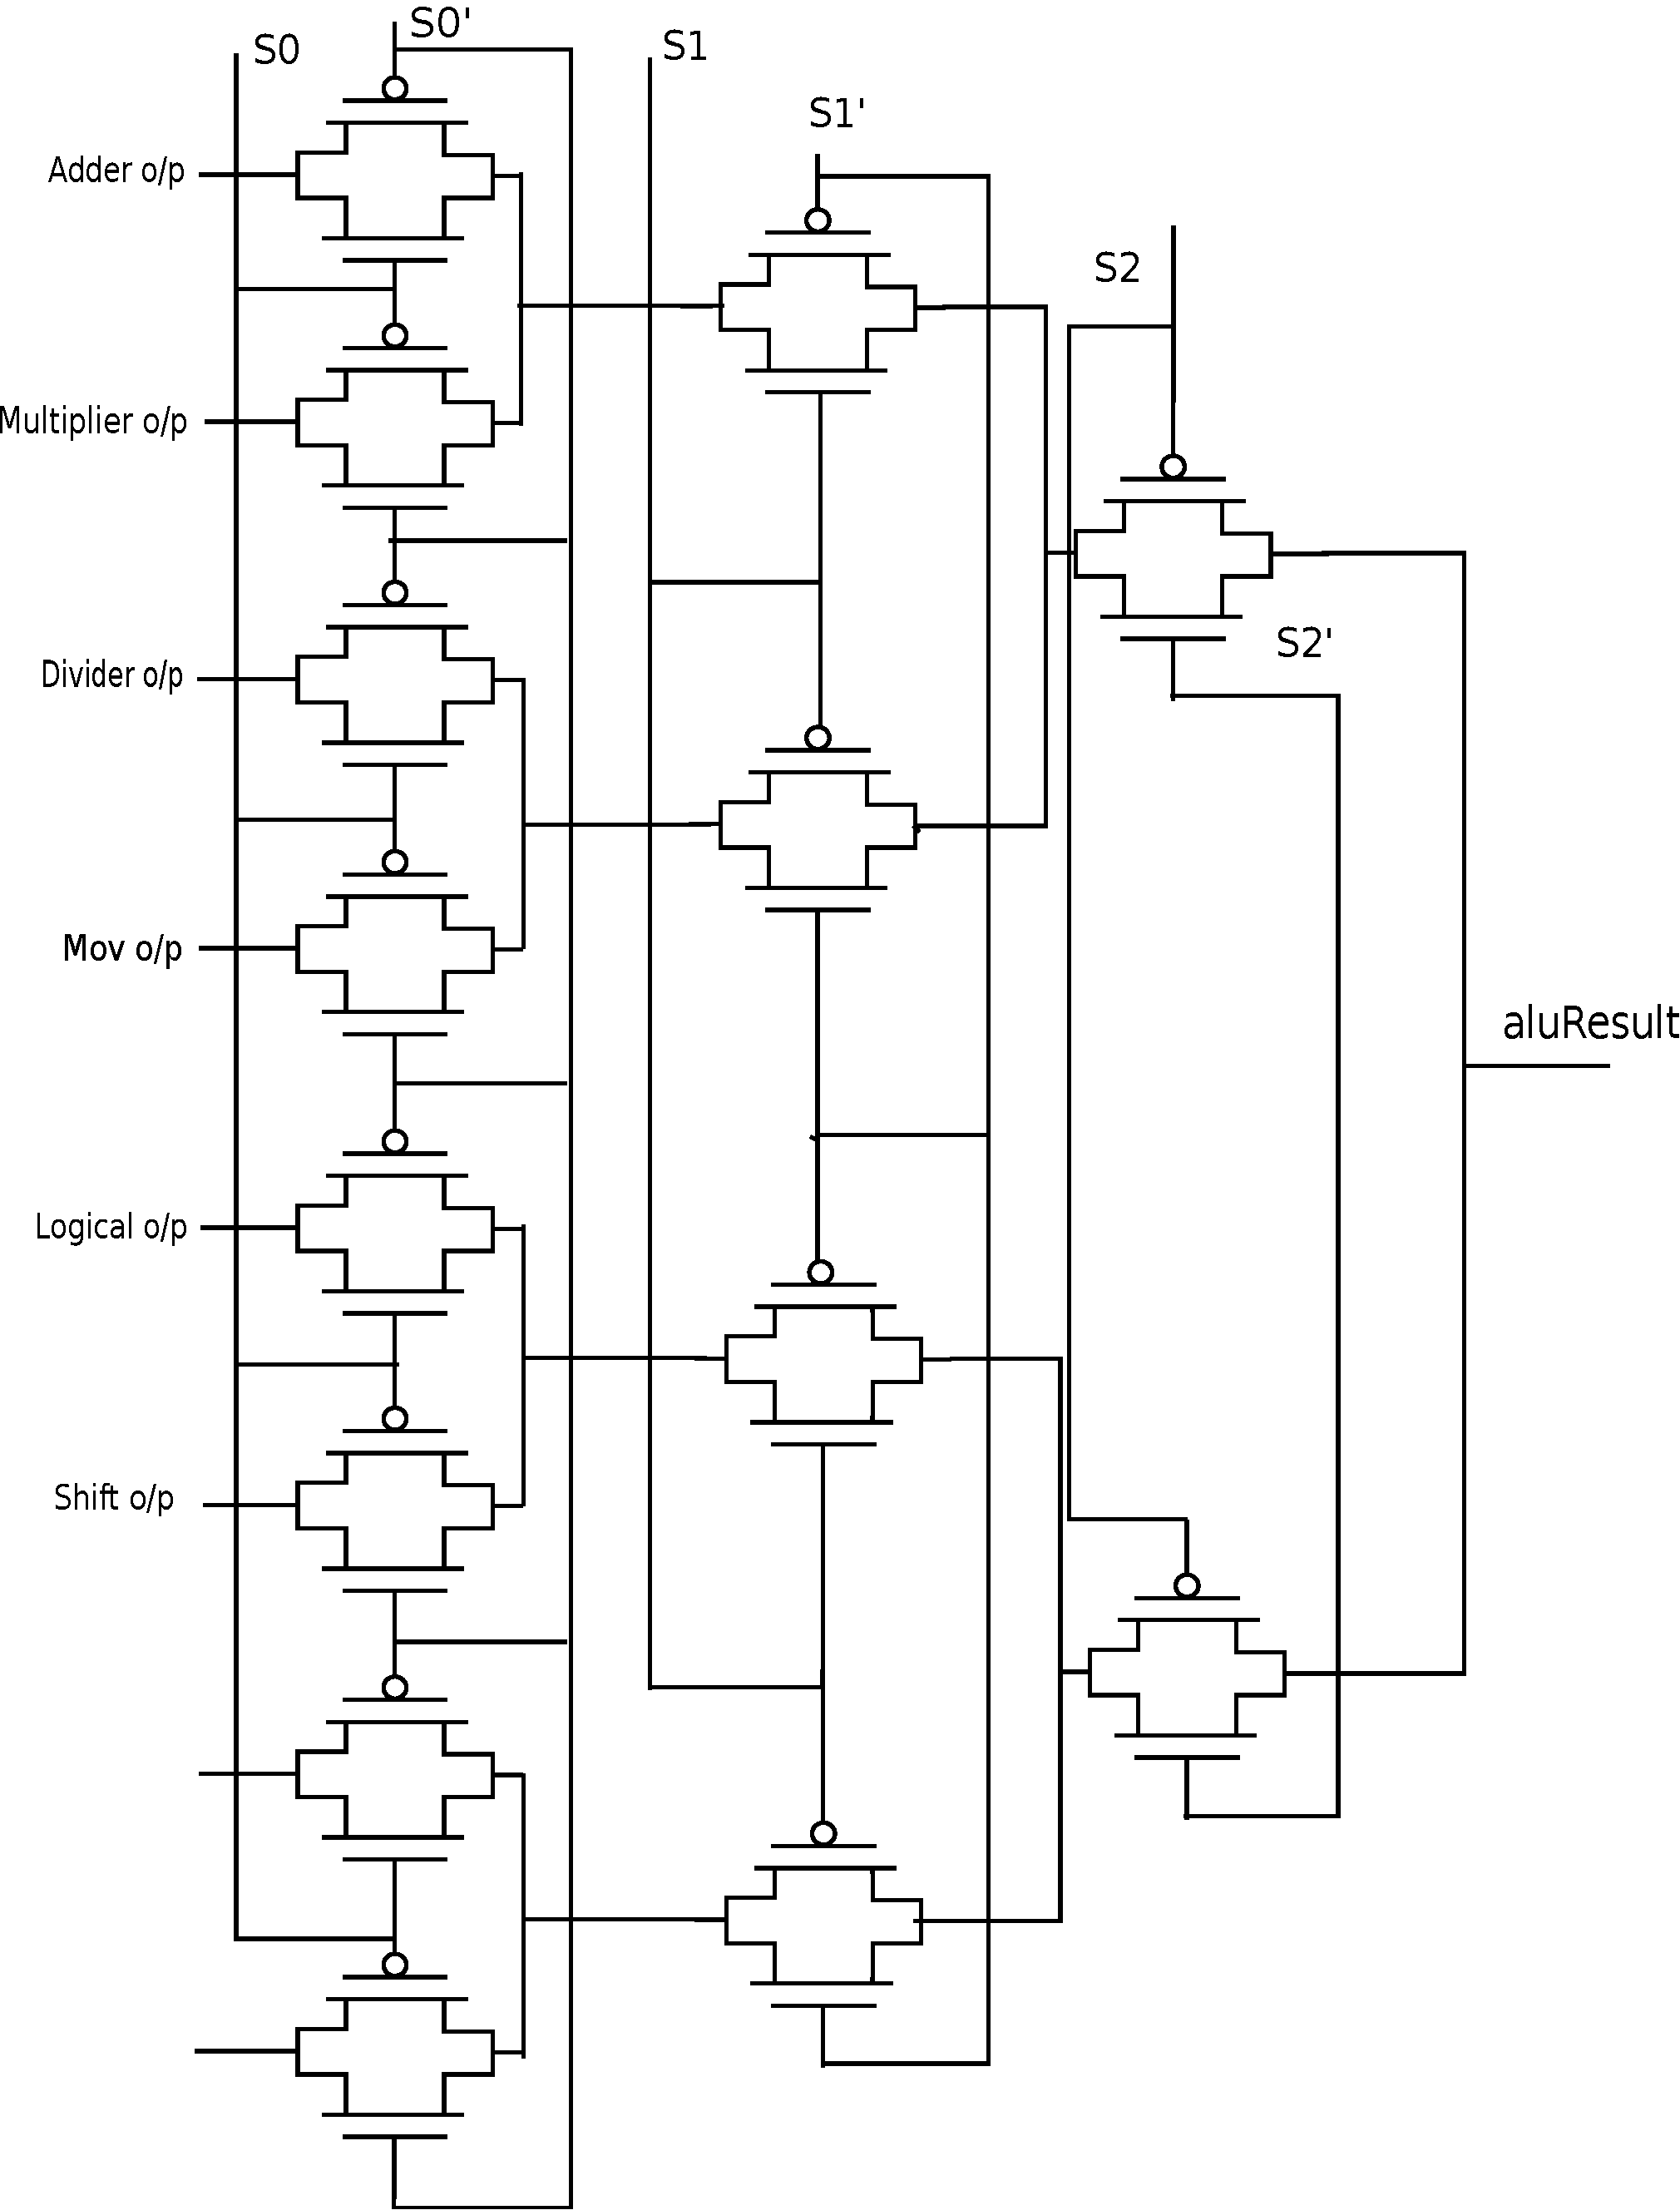
\includegraphics[width=10cm,height=14cm,keepaspectratio]{alu.pdf}
\end{figure}
\Exercise
Draw a circuit for implementing the $cmp$ instruction. It should show the subtraction, and the logic
for updating the flags.
\begin{figure}[H]
  \centering
  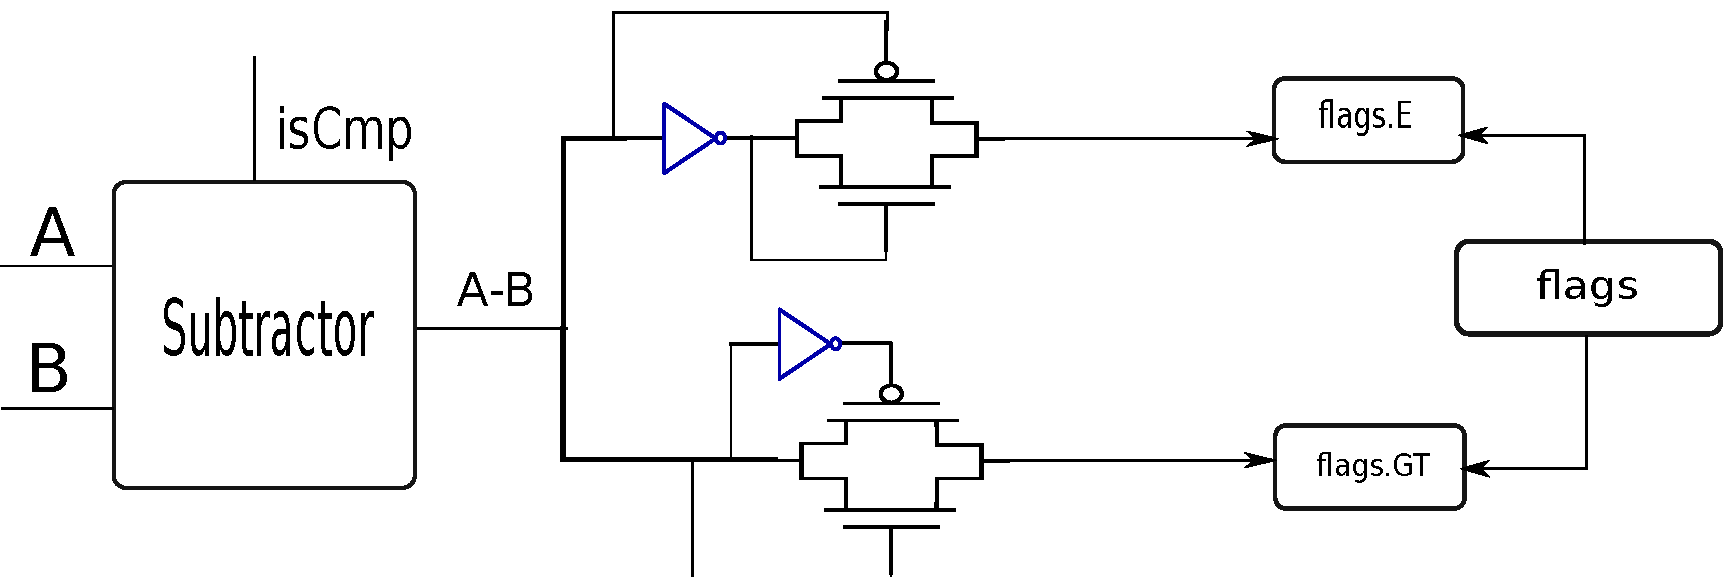
\includegraphics[width=10cm,height=7cm,keepaspectratio]{cmp.pdf}
\end{figure}
\Exercise
How do we implement the $call$ instruction in our processor?
\Answer
The call instruction is 1-address instruction as it takes only one argument-the label of the first instruction of the function. It transfers the control to the label and saves the return address in register \textit{ra}.
For the call instruction, the \textit{isBranchTaken} signal is turned on, and using the value of the \textit{branchPC} from the decode unit, the value of \textit{pc} register is updated.
The \textit{branchTarget} value is calculated using the 27 bit offset in instruction. This is shifted by 2 bits to get a 29 bit number which is then sign extended to obtain a 32 bit offset. This is added to the value in the \textit{pc} register to obtain the address of the function.
The return address is equal to the PC of the \textit{call} instruction plus 4. In the Register Writeback unit, we use a multiplexer to choose between the  \textit{aluResult}, \textit{ldResult},PC plus 4. For the \textit{call} instruction,
the \textit{isCall} is equal to 1, and hence we choose PC + 4. This is written back to the register file.

\Exercise
Show the circuit diagram for computing the $isWb$ signal.
\begin{figure}[H]
  \centering
  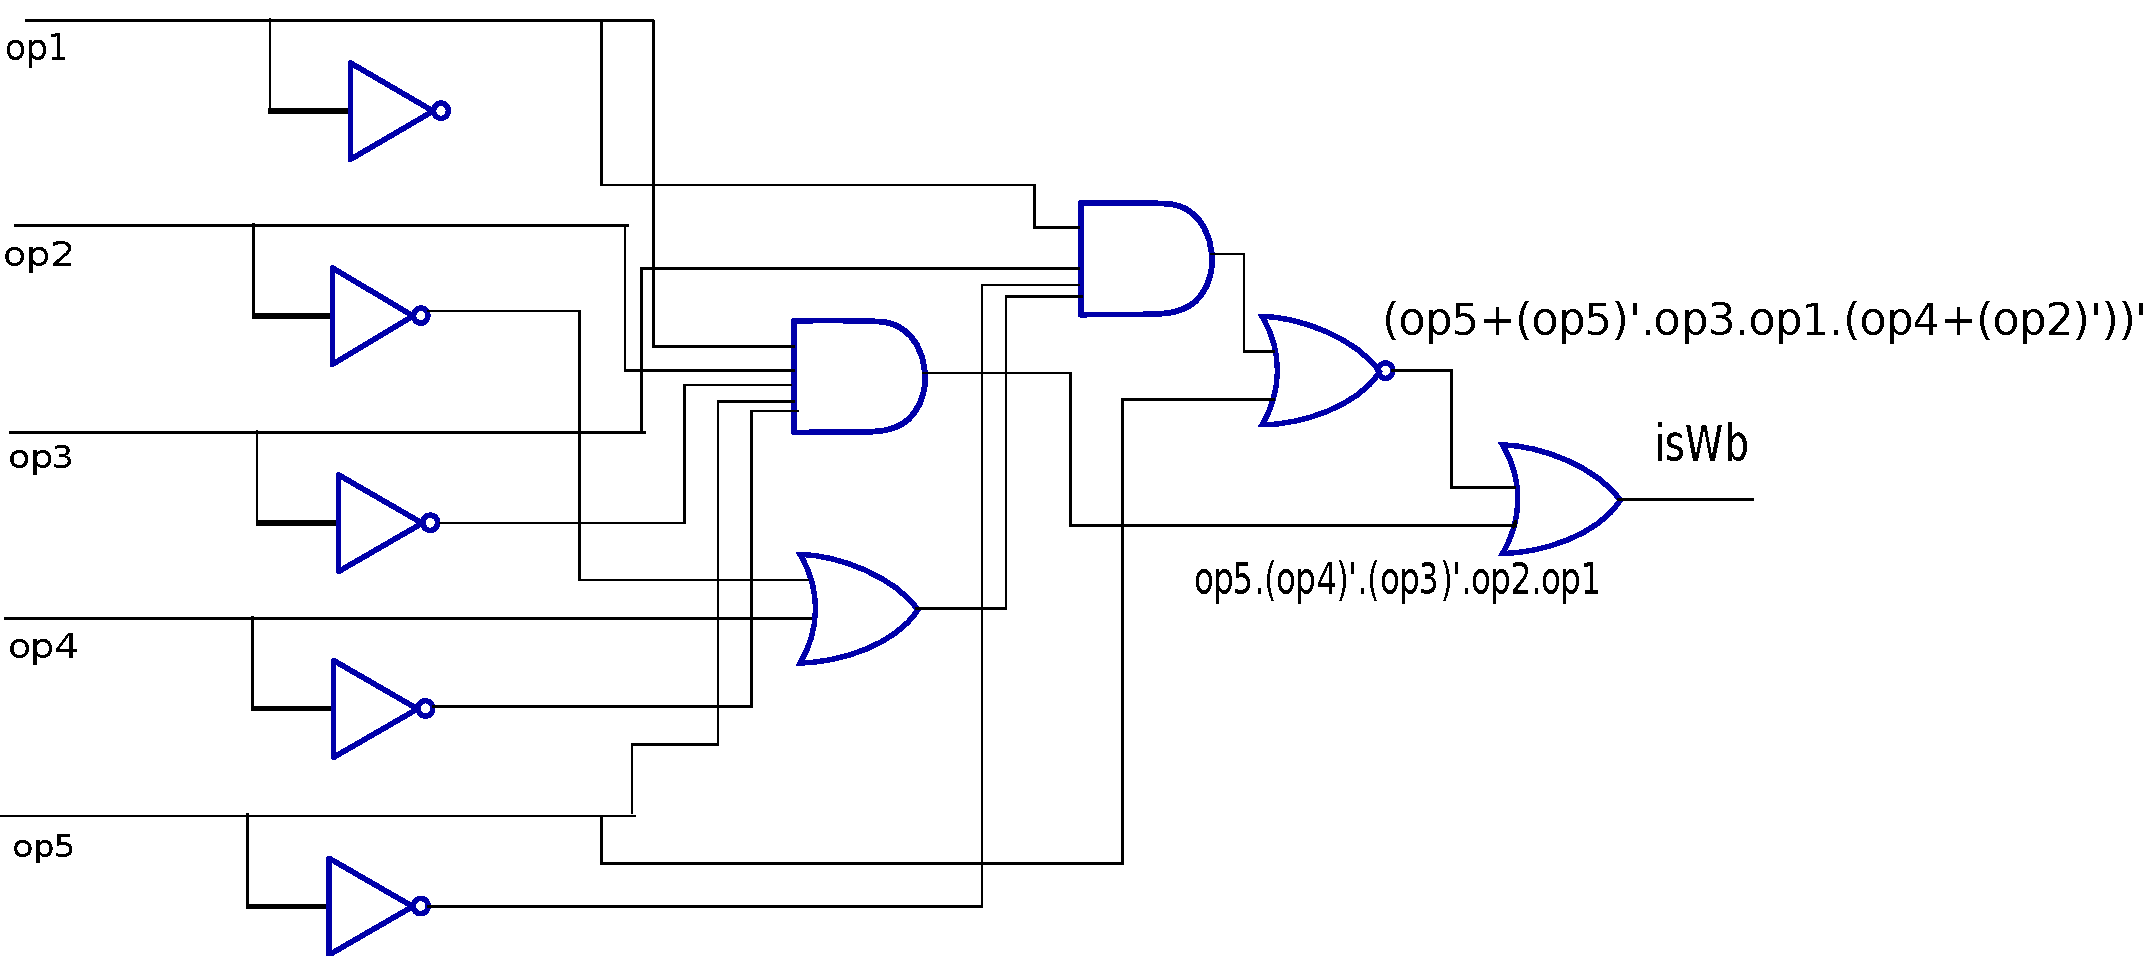
\includegraphics[width=10cm,height=7cm,keepaspectratio]{isWb.pdf}
\end{figure}
\Exercise
Why do we use the $isAdd$ control signal for the load, and store instructions also?

\Answer
The \textit{ld} and \textit{st} instructions use the values - \textit{rd,rs1} and \textit{imm}. The load instruction computes the memory address by computing the sum of contents of \textit{rs1} and \textit{imm}, which is done by the adder of the ALU in the execute stage. It then accesses the memory address and loads its contents to the \textit{rd} register.
The store instruction stores the value of \textit{rd} into the memory address given by contents of \textit{rs1} + \textit{imm}. To compute this, it uses the adder of the ALU in the execute stage.
Hence, for both these instructions, we use \textit{isAdd} control signal to enable the adder of the ALU.
\end{ExerciseList}

\section*{Microprogramming}

\begin{ExerciseList}

\Exercise Compare a hardwired control unit and a microprogrammed control unit.
\Answer
A hardwired processor has a datapath with all the elements required to process and execute an instruction. To incorporate the choice between two input operands, a multiplexer , controlled by a signal from the control unit is added. The control unit takes the instruction contents , and generates all the control signals. 

A microprogrammed processor uses a translation table that translates instructions in the ISA to a set of simple microinstructions. Each microinstruction has access to all the latches, and internal state elements of a processor. The functionality of an instruction is realised by the execution of the set of microinstructions associated with it. These are called \textit{microcodes} and are stored in a microcode table, which can be modified.

Hardwired processors are high performance processors and are used for devices where speed is crucial. However, this comes with a cost on flexibility. Introduction of new instructions or modifying the method of execution of an existing instruction is not possible once designed and shipped.

On the other hand, microprogrammed processors are flexible as the contents of the microcode table can be modified. This flexibility allows addition of new instructions or alteration of method of execution of existing ones. However, the speed is reduced in comparison to the hardwired processors. 
\Exercise Draw the block diagram of a microprogrammed processor.

\begin{figure}[H]
  \centering
  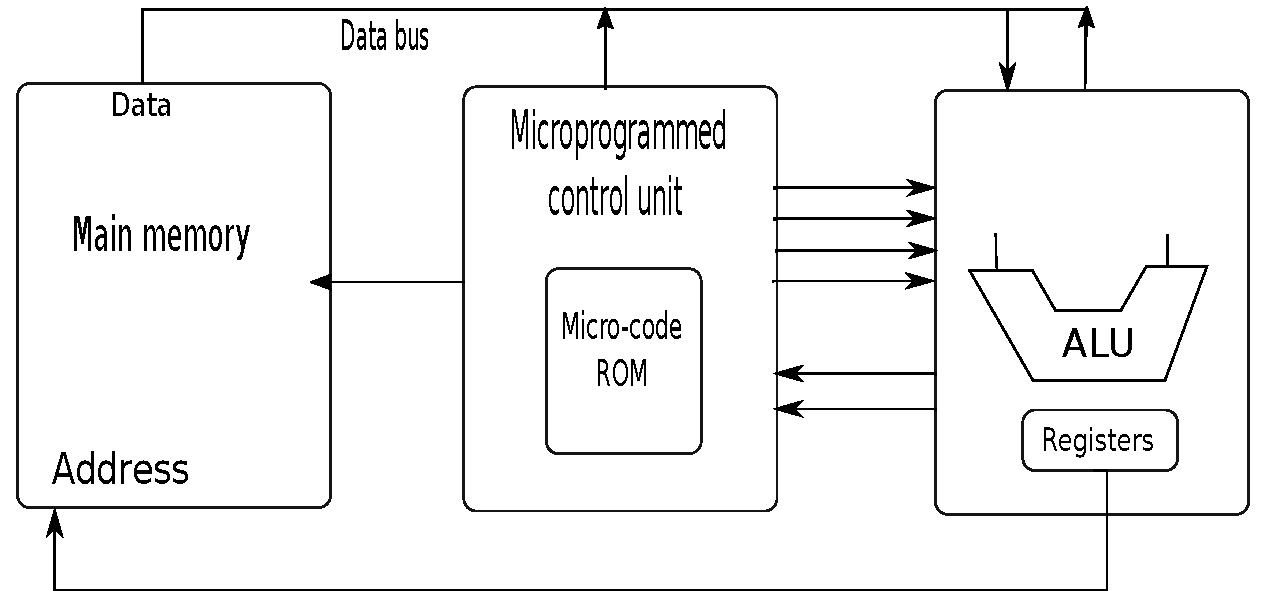
\includegraphics[width=10cm,height=7cm,keepaspectratio]{mcu.pdf}
  \caption{Block diagram of microprogrammed processor}
\end{figure}

\Exercise Why do we need the $mswitch$ instruction.
\Answer
The microprogrammed processor has a set of microinstructions associated with every instruction. These are stored in the microcode table. Once the contents of the instruction are loaded into the \textit{ir} register using \textit{mloadIR} microinstruction, and is decoded using \textit{mdecode}, we need to load the microinstructions corresponding to the instruction being referred to. This is accomplished by using the \textit{mswitch} instruction.
It makes the $\mu$ control unit to jump to the appropriate location in the microinstruction memory, and starts executing microinstructions starting from that location. 
\Exercise
Show the microcode implementation of the load and store instructions.
\Answer :

.begin\newline
mloadIR\newline
mdecode\newline
add pc,4\newline
mswitch\newline
\newline
ld instruction :\newline

/* transfer rs1 to register A*/\newline
mmov regSrc,rs1, $\langle$ read $\rangle$ \\
mmov A,regVal\newline
\newline
/* calculate the effective address */\newline
mmov B,immx, $\langle$ add $\rangle$ /* ALU operation */ \\
\\
/* perform the load */\newline
mmov mar,aluResult, $\langle$ load $\rangle$ \\
\newline
/*write the loaded value to the register file */\\
mmov regData,ldResult\newline
mmov regSrc,rd, $\langle$ write $\rangle$ \\
\newline
/* jump to the beginning */\newline
mb .begin \newline
\newline

The value of the first source register is transferred to the ALU. Then,the value of the immediate is transferred to the second ALU register(B), and the add operation to calculate the effective address is initiated. Once the effective address is calculated, it is available in \textit{aluRegister}. The contents of the \textit{aluRegister} are moved to the memory address register \textit{mar}, and the load operation is initiated. The result is available in the \textit{ld} register in the next cycle. This is then written to the register specified by \textit{rd} in the next two cycles.\newline
\newline
st instruction :
\newline

/* transfer rs1 to register A*/\newline
mmov regSrc,rs1, $\langle$ read $\rangle$ \newline
mmov A,regVal\newline
\newline
/* calculate the effective address */\newline
mmov B,immx, $\langle$ add $\rangle$ /* ALU operation */\newline
\newline
/* perform the store */\newline
mmov mar,aluResult\newline
mmov regSrc,rd, $\langle$ read $\rangle$\newline
mmov mdr,regVal,$\langle$ store $\rangle$\newline
\newline
/* jump to the beginning */\newline
mb .begin \newline \\
The store function works in a similar way. The effective memory address is first calculated and stored in the \textit{mar} register. Then, the value of the \textit{rd} register that contains the data to be stored is read. This, in turn, is saved to the \textit{mdr} register, and the store operation is issued.
\Exercise
Write a program in microassembly to check if a number in register $r2$ is a perfect square. Save the Boolean result
in register, r0.
\Answer :

.begin\newline
mloadIR\newline
mdecode\newline
add pc,4\newline
mswitch\newline \\
mmovi B,1   /*stores the odd number being added*/\newline
mmovi regSrc,2,$\langle$ read $\rangle$\newline
mmov A,regVal\newline \\
/*loop*/\newline
.loop:\newline
/*Compute subtraction*/\newline
mmov A,A,$\langle$ sub $\rangle$\newline
mmov A,aluResult\newline
madd B,1    /*B=B+1*/\newline
madd B,1    /*B=B+1*/\newline
mbeq A,0,.success   /*n =1+3+5+7.. , hence is a perfect square, branch to .success*/\newline
mmov sr1,A\newline
mmov sr2,B\newline
mmovi A,0   /*A=0*/\newline
mmov B,sr2,$\langle$ cmp $\rangle$\hspace{3mm}/*B=sum of odd numbers*/\newline
mbeq flags.GT,1,.failure  /*If the sum of odd numbers exceeds n, then n is not a perfect square, branch to .failure*/\newline
mmov A,sr1\newline
mmov B,sr2\newline
mb .loop\newline
\newline
.success:\newline
mmovi regSrc,3\newline
mmovi regData,1,$\langle$ write $\rangle$\newline
mb .begin\newline
\newline
.failure:\newline
mmovi regSrc,3\newline
mmovi regData,0,$\langle$ write $\rangle$\newline
mb .begin\newline \\ \\

The program uses the logic that a perfect square can be expressed as a sum of odd numbers 1+3+5+7+9... .Thus, from the original number, we keep subtracting every odd number beginning from 1. If we end up with a zero, then the given number is a perfect square. However, if it turns out to be a negative number, then it isn't. Hence, we break out of the loop in either case and branch to different functions.\newline
Assumption: sr1 and sr2 are scratch registers

\Exercise
Write a program in microassembly to check if the value in register $r2$ is a palindrome. A palindrome
reads the same from both sides. For example, the 8 bit number, 11011011 is a palindrome. Save the Boolean result
in register, r0.
\Answer:

.begin\newline
mloadIR\newline
mdecode\newline
add pc,4\newline
mswitch\newline \\
mmovi B,0  /*Loading count into B*/\newline
mmovi regSrc,2,$\langle$ read $\rangle$\newline
mmov A,regVal\newline \\ 
mmov sr2,B  /*sr2 holds the value of count*/\newline
mmov sr1,A  /*sr1 holds the value of original number*/\newline
mmovi A,1   /*To perform 1 $\ll$ count*/ \\
.loop:\newline
mbeq sr2,16,.success /*breaking out of loop if count==16*/\newline
mmov B,B,$\langle$ lsl $\rangle$  /*aluResult=1 $\ll$ count*/\newline
mmov sr2,B  /*sr2 holds count*/\newline
mmov A,aluResult  /*A=aluResult*/\newline
mmov B,sr1,$\langle$ and $\rangle$    /*x=num and (1 $\ll$ count)*/\newline
mmov sr3,aluResult  /*sr3 holds lsb*/\newline \\
mmovi A,31\newline
mmov B,sr2,$\langle$ sub $\rangle$   /*aluResult=31-count*/\newline
mmov B,aluResult\newline
mmov A,sr1,$\langle lsr \rangle$  /*aluResult=(num $\ll$ (31-count))*/\newline
mmov A,aluResult\newline
mmovi B,1,$\langle and \rangle$ \hspace{3mm}/*y=(num $\gg$ (31-count)) $\and$ 1*/\newline \\
madd sr2,1 /*count=count+1*/\newline
mmovi A,1  /*A=1*/\newline
mmovi B,sr2  /*B=count*/\newline
mbeq sr3,aluResult,.loop  /*Loop if x==y */\newline
/*x and y are count th bits from left and right*/\newline
.failure\newline
mmovi regSrc,3\newline
mmovi regData,0,$\langle write \rangle$ \newline
mb .begin\newline
.success\newline
mmovi regSrc,3\newline
mmovi regData,1, $\langle write \rangle$ \newline
mb .begin\newline    
\newline
Assumption: sr1,sr2 and sr3 are scratch registers
\Exercise[difficulty=1]
Write a program in microassembly to check if the value in register $r2$ can be expressed as a sum of two
cubes in two different ways. For example, 1729, is one such number. $1729 = 12^3 + 1^3 = 10^3 + 9^3$. Save the Boolean result
in register, r0.

\Exercise
Outline the design of the shared bus, and microprogrammed data path. Explain the functionalities of each of its
components.
\Answer
The shared bus consists of two buses - write bus and read bus.\newline
The first bus,\textit{write bus} is connected to all the registers that might write data into the bus. The output of the write bus,the embedded immediate($\mu$ imm) in the microinstruction, and the output of the $\mu$adder are sent to a multiplexer. The $\mu$adder adds the embedded immediate with the register contents. Now, this multiplexer chooses one value among the three, and sends it onto a read bus. This multiplexer is referred to as \textit{transfer multiplexer}. All the registers that might potentially read a value are connected to the read bus. The PC is connected to both the buses. The $\mu$adder has two inputs. One of them is the sign extended immediate that is a part of the microinstruction, and the other is the output of the write bus.\newline
The value sent on the write bus is compared with $\mu$imm . The result is contained in the \textit{isMBranch} signal. This is required for the implementation of \textit{mbeq} instruction.
\newline \textbf{Microprogrammed Datapath}\newline \\
1.\hspace{4mm}\textit{Fetch Unit}:\newline 
It consists of two registers-\textit{pc} and \textit{ir}, PC and instruction register respectively.\textit{ir} contains the contents of the instruction. The \textit{pc} register can read or write to the bus. The \textit{pc} is connected to the instruction memory and bus. \textit{ir} is connected only to the instruction memory.\newline \\
2.\hspace{4mm}\textit{Decode Unit}:\newline 
The decode unit breaks the instruction contents into multiple fields, and exports as registers-\textit{I,rd,rs1,rs2,immx,branchTarget}. The offset from the current PC is calculated by extracting [1:27] bits from the instruction register \textit{ir}, and shifting by two places. The offset thus calculated ,is added to the PC.\newline \\
3.\hspace{4mm}\textit{Register File}:\newline 
It has two source registers-\textit{regSrc} and \textit{regData}.The \textit{regSrc} register contains the number of the register to be accessed.In case of a write,the \textit{regData} register contains the value to be written. The \textit{args} values are directly read from the bus. They contain the commands to the register file-\textit{read,write,nop}.If \textit{args} specifies a \textit{write} operation,then the value in the \textit{regData} is written to the \textit{regSrc}.If its a \textit{read} operation, then the register specified by \textit{regSrc} is read and stored in \textit{regVal}.\newline \\
4.\hspace{4mm}\textit{ALU}:\newline 
The ALU consists of two registers, A and B.The ALU performs actions on the values contained in the registers,A and B. The nature of the operation is specified by the \textit{args} value. For all other instructions other than \textit{cmp}, the result is stored in the \textit{aluResult}, whereas for \textit{cmp}, it gets stored in either of the two registers-\textit{flags.E},\textit{flags.GT}.\newline \\
5.\hspace{4mm}\textit{Memory Unit}:\newline 
It has two source registers-\textit{mar,mdr}.The memory address register buffers the memory address, and memory data register buffers the value to be stored.If the operation specified by \textit{args} is a load, then the result is stored in \textit{ldResult}.\newline
 
\Exercise
Draw a detailed diagram of the $\mu$control unit along with the transfer multiplexer in a vertically microprogrammed
processor.
\begin{figure}[H]
  \centering
  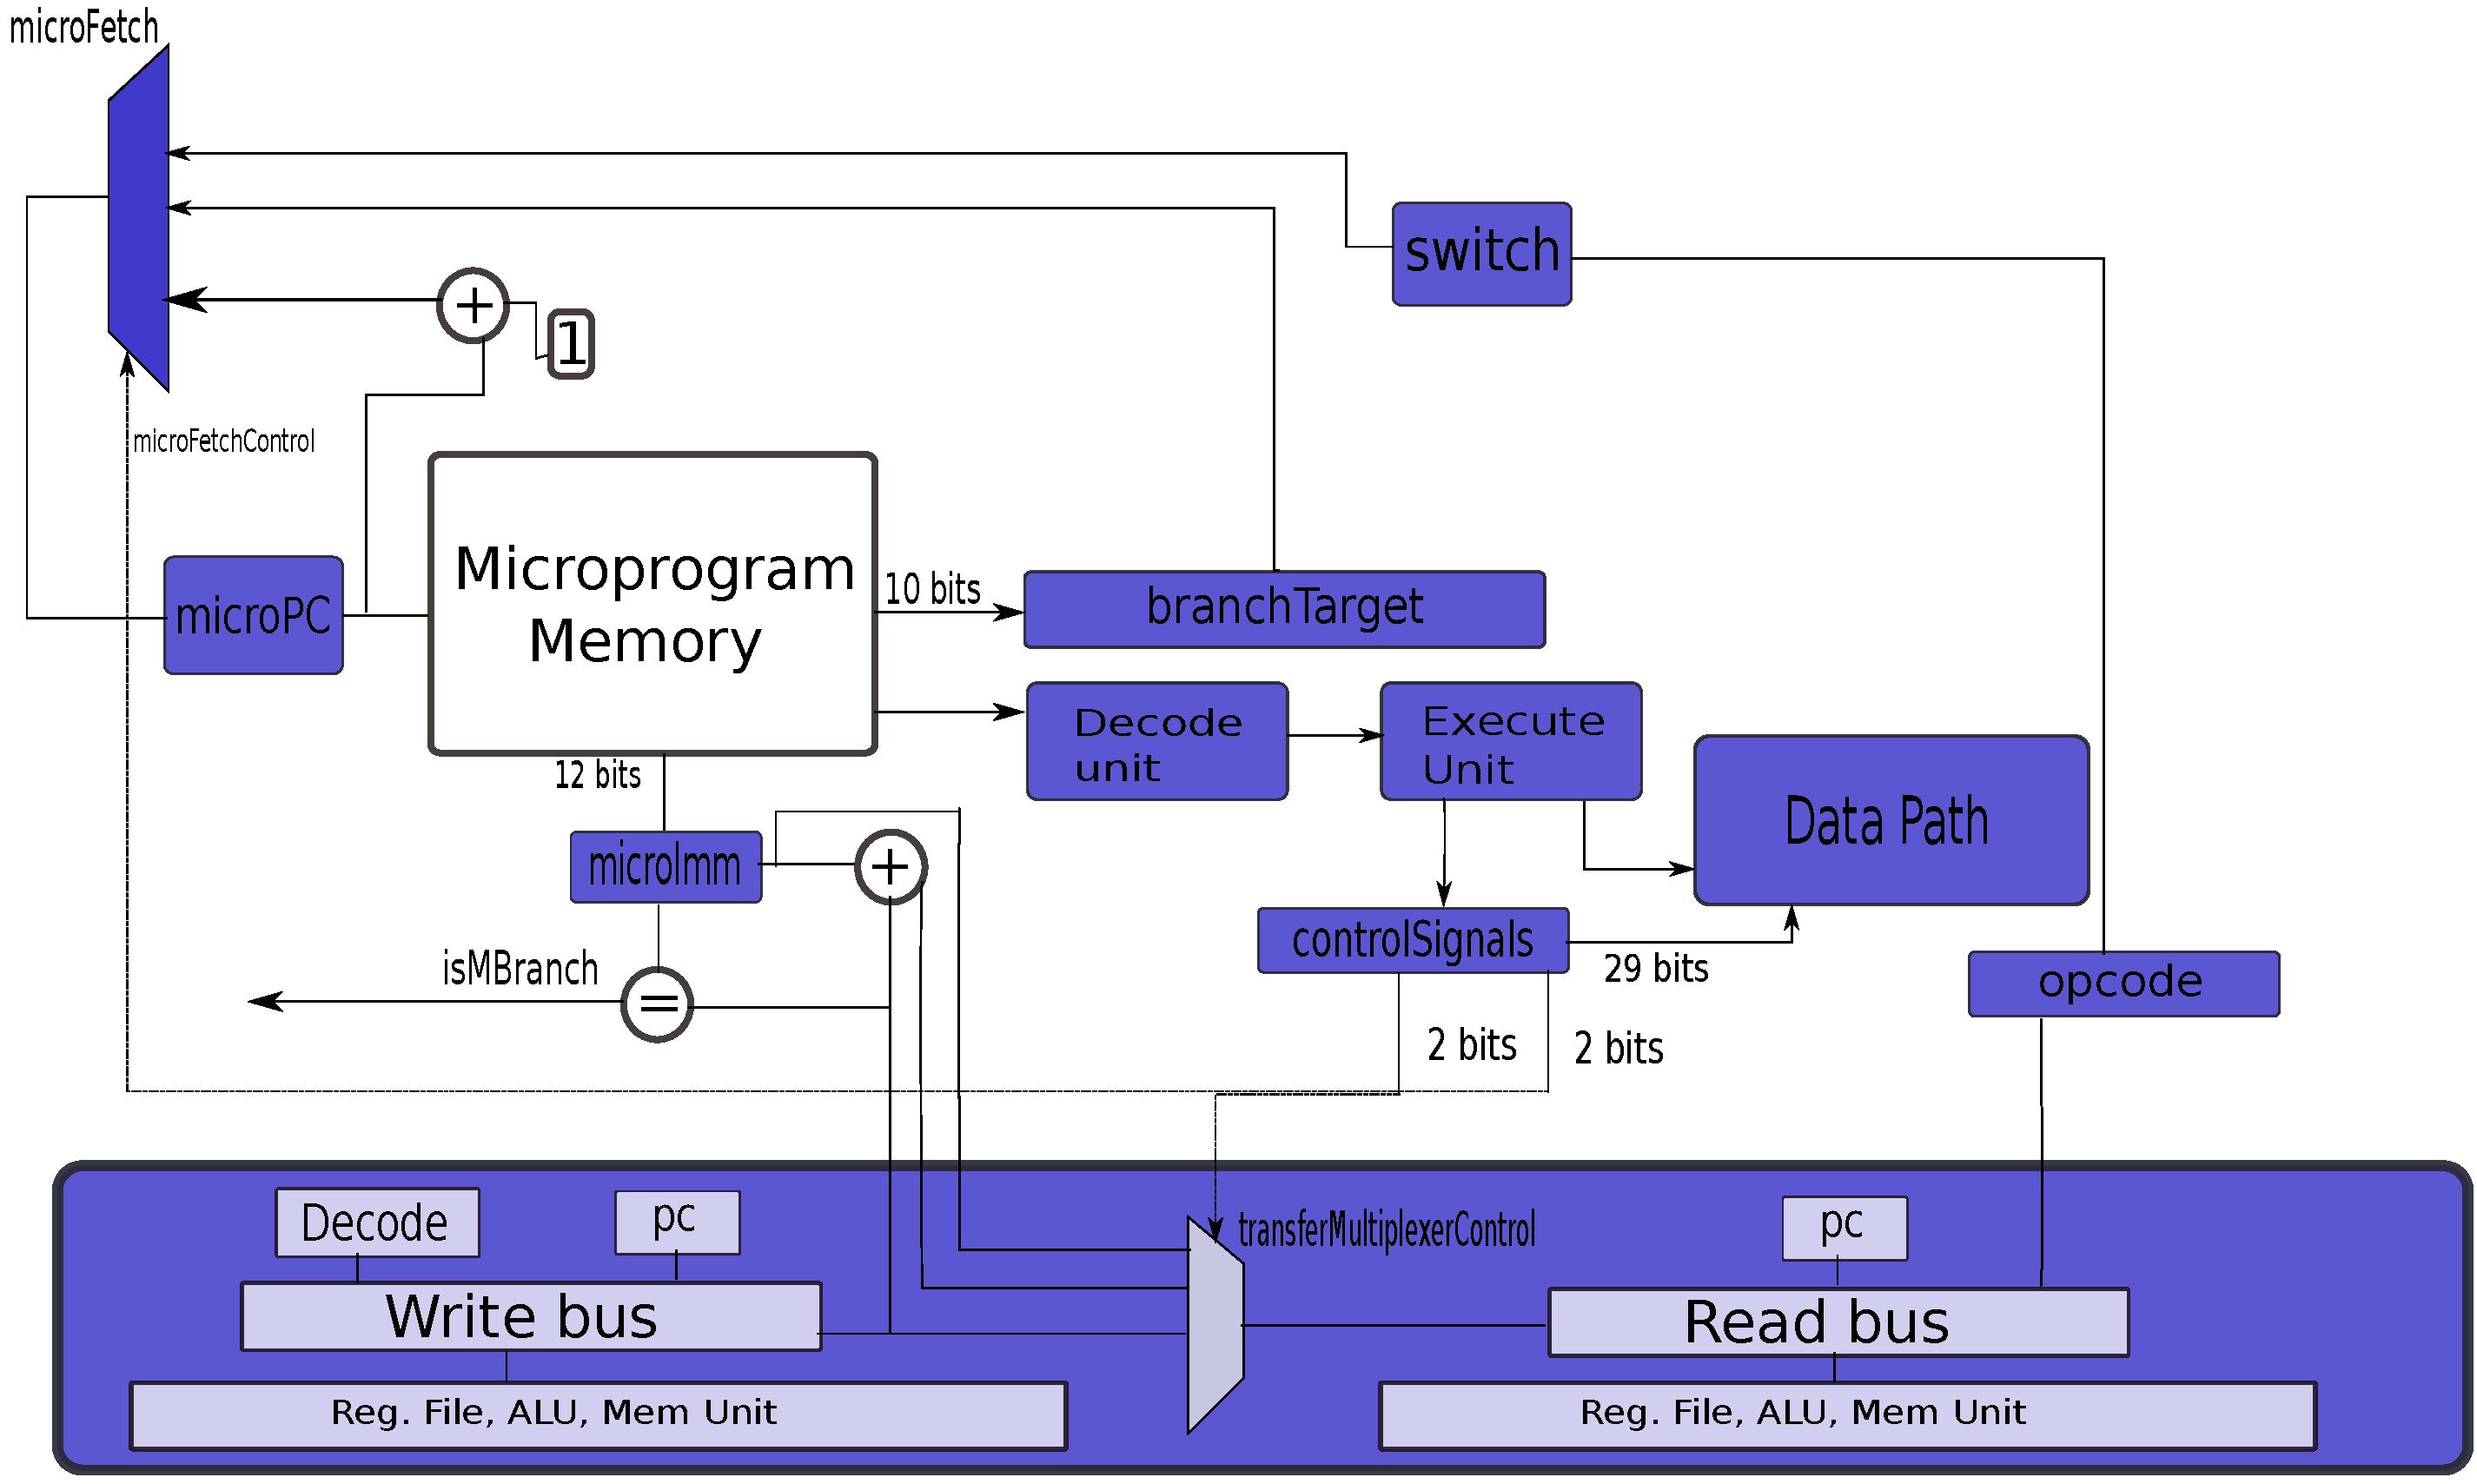
\includegraphics[width=12cm,height=14cm,keepaspectratio]{verticalMP.pdf}
\end{figure}
\Exercise
Draw a detailed diagram of the $\mu$control unit along with the transfer multiplexer in a horizontally microprogrammed
processor.
\begin{figure}[H]
  \centering
  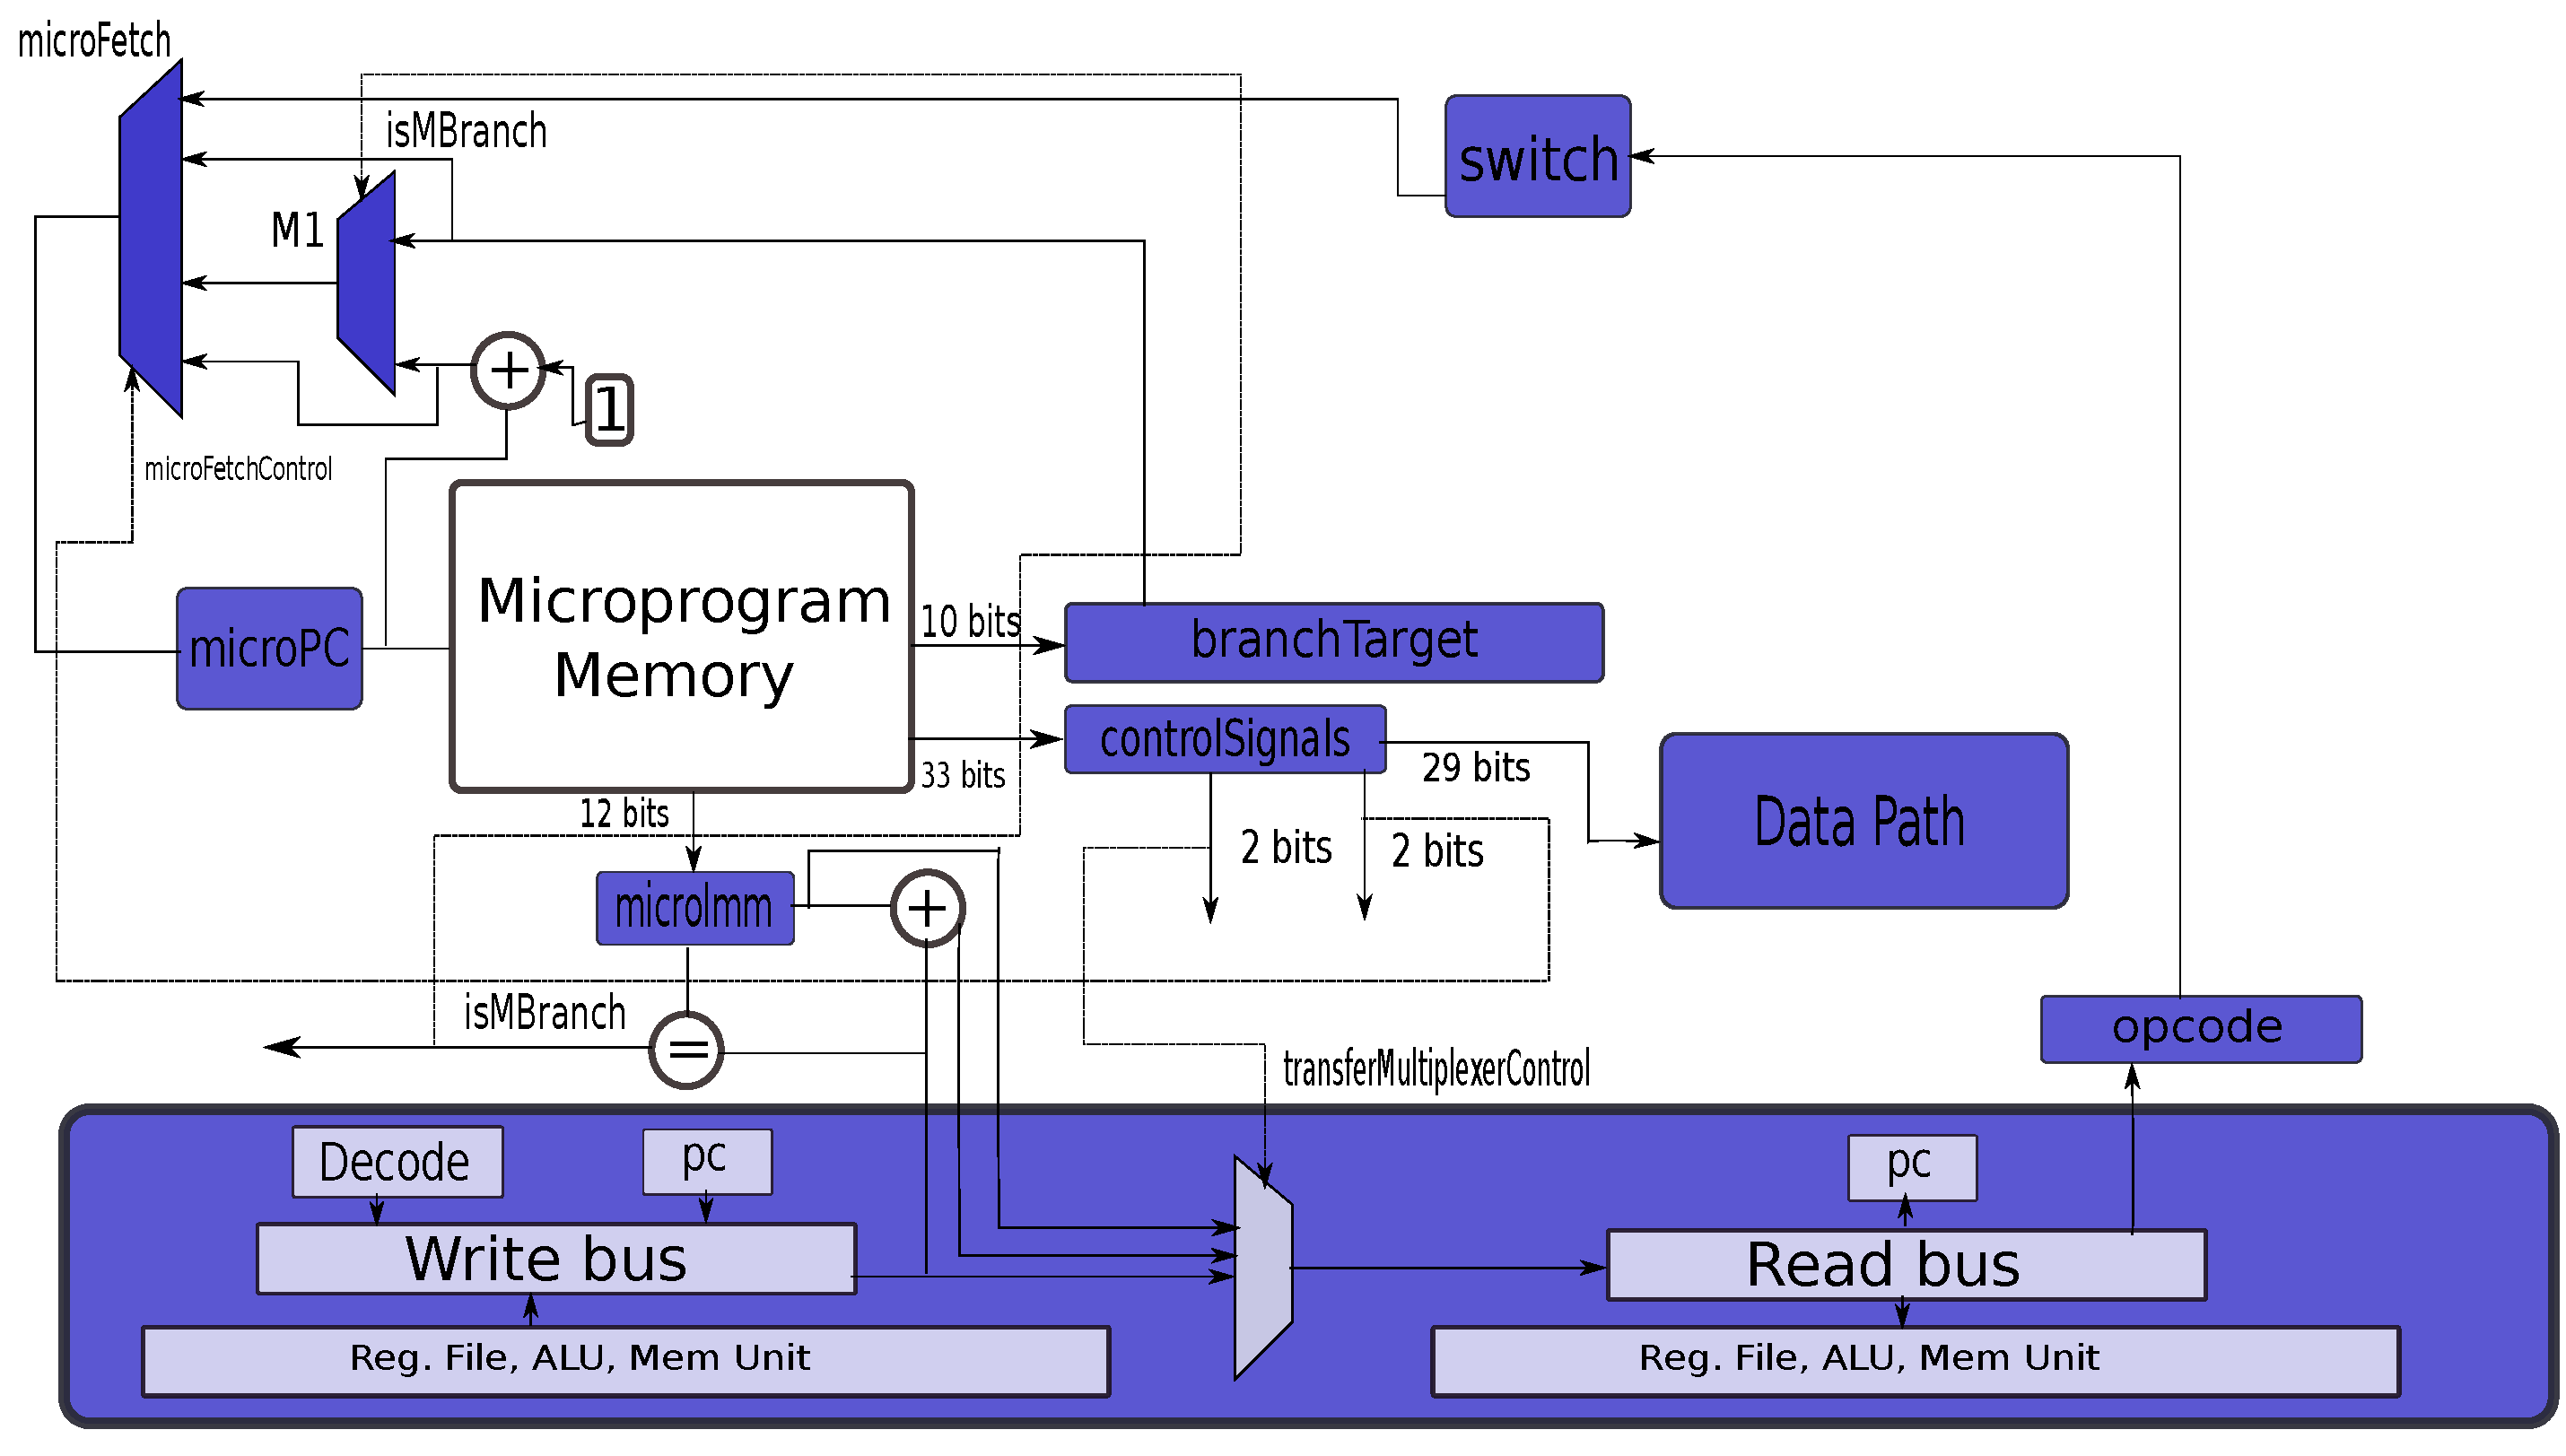
\includegraphics[width=12cm,height=14cm,keepaspectratio]{horizontalMP.pdf}
\end{figure}
\Exercise Compare the tradeoffs between horizontal and vertical microprogramming.
\Answer The tradeoffs between horizontal and vertical microprogramming are:\newline
1. Horizontal microprogramming requires more storage since it requires 65 bits for every instruction, when compared to that of 45 bits in vertical microprogramming. \newline
2. Horizontal microprogramming eliminates the need for dedicated signal generation logic in the $\mu$control unit.\newline
3. To program a horizontally microprogrammed processor, it is necessary to expose the control signals to the programmer and microassembler.This makes the microassembler specific to the processor. However, in case of vertical microprogramming, as long as the internal register set remains the same, we do not need different microassemblers.\newline
\end{ExerciseList}

\section*{Design Problems}

\begin{ExerciseList}
\Exercise
Implement the hardwired \simplerisc processor using Logisim, which is an educational tool for designing
and simulating digital circuits. It is freely available at \url{http://ozark.hendrix.edu/~burch/logisim}. 
Try to support all the instructions, and the modifiers.

\Exercise Now, try to implement a horizontally microprogrammed processor using Logisim. This project has
two parts.
\begin{enumerate}[a)]
\item Write a microassembler that can translate microassembly instructions to machine instructions. Use
this microassembler to generate the microcode for all the instructions in the \simplerisc ISA.
\item Create a data path and control path in Logisim for a horizontally microprogrammed processor.
This processor should be able to directly execute the code generated by the microassembler.
\item Run regular \simplerisc programs on this processor. 
\item Implement custom \simplerisc instructions such as $multiply-add$ (a $\leftarrow$ b*c + d), or instructions
to find the square of a number on this processor.
\end{enumerate}

\Exercise 
Implement the basic hardwired processor in a high level description language such as VHDL. You can use the
freely available open source tool, GNU HDL (\url{http://gna.org/projects/ghdl/}), to implement, and simulate
your circuit.

\end{ExerciseList}







































\newpage
\chapter{Principles of Pipelining}
\begin{flushright}
\textbf{Solutions prepared by Prajwala TM $<$prajwala.tm@gmail.com$>$}
\end{flushright}
\section*{Exercises}
\vskip 1cm

\setcounter{Exercise}{0}
\setcounter{Answer}{0}

\section*{Pipeline Stages}

\begin{ExerciseList}

\Exercise
Show the design of the IF, OF, EX, MA, and RW pipeline stages.
Explain their functionality in detail.
\Answer
\hspace{3mm} \\
1.\textit{IF Stage}:\\
The only additions to the IF Stage is a pipeline register where we save the value of the PC, and contents of the instruction. This is the only information required for the subsequent stages. \\
2.\textit{OF Stage}: \\
The extra additions are the connections to the two pipeline registers IF-OF, and OF-EX. It extracts the fields $rd$,$rs1$,$rs2$, and the immediate from the instruction. These are sent to the register file, the immediate and branch units. We send the contents of the instruction to the control unit that generates the control signals. Only three control signals-\textit{isRet,isImmediate,isSt} are used immediately. The rest of the control signals are used for controlling multiplexers in the subsequent stages of the pipeline. Hence, they are saved in the OF-EX pipeline register. All these control signals are saved and some space is allocated in the instruction packet called $control$. The intermediate results generated also need to be carried. The OF stage generates the \textit{branchTarget}, inputs for the ALU, and the value to be written to memory for a store instruction($op2$). Some fields are allocated in the instruction packet for the same.\\
3.\textit{EX Stage}: \\
The ALU receives its inputs A and B from the OF-EX pipeline register. The results generated by this stage are \textit{aluResult}, the final branch target, and branch outcome. The result is added to the instruction packet, and saved in the EX-MA register. The EX-MA register also contains the rest of the fields namely-PC,contents of the instruction, control signals, and second operand read from the register file
($op2$). \\
4. \textit{MA Stage}: \\
The only operand that the load instruction takes is the result of the ALU, which contains the effective memory address. This is saved in the \textit{aluResult} field of the EX-MA register. The data to be stored resides in the $rd$ register. Here, the $op2$ field is connected to the MDR register, and the $aluResult$ is connected to the MAR register. The control signals-$isLd$ and $isSt$ are also a part of instruction packet, and they are routed to the memory unit. The output of this stage is the result of the load instruction and is saved in the $ldResult$ field of the MA-RW register. \\
5.\textit{RW Stage}: \\
The values of the $aluResult$ and $ldResult$ fields are the inputs this stage requires. These inputs along with next default PC are connected to the multiplexer that chooses the value to be written back. It does not have any pipeline register, since it is the last stage of the pipeline. \\
\Exercise
Why do we need to store the $op2$ field in the instruction packet? Where is it used?
\Answer
The $op2$ field contains the value to be written to memory for a store instruction. The OF stage generates the value of $op2$ by reading contents of the second register. This is thus saved, in the instruction packet at this stage and transferred to the subsequent pipeline stages. It is used in the MA stage, where $op2$ is connected to the MDR register, and is written to the memory address specified by $aluResult$, connected to the MAR. \\
\Exercise
Why is it necessary to have the $control$ field in the instruction packet?
\Answer
In the OF stage, we send the contents of the instruction extracted to the control unit that generates the control signals. Only three control signals-\textit{isRet,isImmediate,isSt} are used immediately. The rest of the control signals are used for controlling multiplexers in the subsequent stages of the pipeline. Hence, they are saved in the OF-EX pipeline register. All these control signals are saved and some space is allocated in the instruction packet called $control$. This is used later in the pipeline. \\
\Exercise
Why do we require latches in a pipeline? Why are edge sensitive latches preferred?
\Answer
We need to design a method that ensures that instructions seamlessly proceed to the subsequent pipeline stage. There is need for a global mechanism that ensures all the instructions proceed to the next stages simultaneously. This can be achieved with the help of a clock. For this purpose, we insert a register between every two consecutive pipeline stages. Each of these are called pipeline latches, or pipeline registers. \\
These are controlled by the falling edge/rising edge of the clock for defining a specific timing such that all the instructions simultaneously proceed to the next stage. Such pipeline latches are called edge-triggered latches. They are preferred over level triggered latches for more accurate results. \\ 
\Exercise
Why is it necessary to split the work in a data path evenly across the pipeline stages?
\Answer
The work in a data path should be evenly split across the pipeline stages to minimise the idleness in the circuit. This ensures that the pipeline is balanced, and the time taken by each stage is approximately the same, and the cycle time can be fixed accordingly. This leads to better performance. \\
\Exercise[difficulty=1]
We know that in an edge sensitive latch, the input signal has to be stable for $t_{hold}$
units of
time after the negative edge. Let us consider a pipeline stage between latches
$L_1$ and $L_2$. Suppose the output of $L_1$ is ready immediately
after the negative edge, and almost
instantaneously reaches the input of $L_2$. In this case, 
we violate the hold time constraint at $L_2$. How can this situation be avoided?
\Answer
The situation can be avoided by adding an additional constraint on the output signal of a latch. The output signal, that is ready should not be transmitted for $t_{hold}$ units of time after the negative edge. In such a case, the output of $L_1$ will not reach $L_2$ for $t_{hold}$ units of time, and the input signal constraint at $L_2$ will not be violated. 
\end{ExerciseList}

\section*{Pipeline Design}

\begin{ExerciseList}
\Exercise
Enumerate the rules for constructing a pipeline diagram.
\Answer
\hspace{3mm} \\
The rules are : \\
1. Construct a grid of cells, which has five rows, and N columns, where N is the total number of clock cycles that we wish to consider. Each of the five rows corresponds to a pipeline stage. \\
2. If an instruction [k] enters the pipeline in cycle $m$, then we add an entry corresponding to [k] in the $m^{th}$ column of the first row. \\
3. In the $(m+1)^{th}$ cycle, the instruction can either stay in the same stage or can move to the next row. We add a corresponding entry in the grid cell. \\
4. In a similar manner, the instruction moves from the IF stage to the RW stage in sequence. It never moves backwards. However, it can stay in the same stage across consecutive cycles. \\
5.We cannot have two entries in a cell. \\
6. We finally remove the instruction from the pipeline diagram after it leaves the RW stage. \\
\Exercise
Describe the different types of hazards in a pipeline.
\Answer
The different types of hazards are : \\ \\
1. \textit{Data hazards}: \\
A data hazard represents the possibilityof erroneous execution because of the anavailability of correct data. Let us consider the following code snippet: 
\begin{Verbatim}
[1]: add r1, r2, r3 
[2]: sub r3, r1, r4 
\end{Verbatim}
Here the add instruction produces the value for register r1 and the sub-instruction uses it as a source operand. Instruction [1] writes the value of r1 in the fifth cycle, and instruction [2] needs to read its value in the third cycle. This is not possible. Such kind of hazard is known as data hazard. There are three types of data hazards - RAW(Read After Write), WAW(Write After Write), WAR(Write After Read). \\ \\
2. \textit{Control hazards}: \\
A control hazard represents the possibility of erroneous execution in a pipeline because instructions in the wrong part of a branch can possibly get executed and save their results in memory, or in the register file.Instructions that would have been executed if a branch would have had an outcome that is different from its real outcome, are said to be on the wrong path. Let us consider the following code snippet: 
\begin{Verbatim}
[1]: beq .foo 
[2]: mov r1,4 
[3]: add r2, r4, r3 
... 
... 
.foo:
[100]: add r4, r1, r2 
\end{Verbatim}
The outcome of the branch is decided in cycle 3, and is communicated to the fetch unit. The fetch unit starts fetching the correct instruction from cycle 4. Now if the branch is taken, then instructions [2] and [3] should not get executed. However, it is not possible to determine the outcome of the branch in cycles 2 and 3. Hence, these instructions will be fetched and will be a part of the pipeline. If the branch is taken, then there is a possibility that instructions [2] and [3] might corrupt the state of the program and introduce an error. These instructions are said to be on the wrong path. This is an example of a control hazard. \\ \\
3. \textit{Structural hazards}: \\
A structural hazard refers to the possibility of instruction not being able to execute because of resource constraints. They arise when multiple instructions try to access a functional unit in the same cycle, and due to capacity limitations, the unit cannot allow all the interested instructions to proceed. In such a case, a few of the instructions in the conflict need to stall their execution. Structural hazards do not arise in \simplerisc pipeline.
\Exercise
In the \simplerisc pipeline, why don't we have structural hazards?
\Answer
In the \simplerisc pipeline, we never have a situation in which multiple instructions across different pipeline stages wish to access the same unit and that unit does not have the capacity to service all the requests. The only units that are accessed by multiple stages are the fetch unit and the register file. The fetchunit is accessed by an instruction in the IF stage, and by branch instructions in EX stage. It is designed to handle both the requests. Likewise, the register file is accessed by instructions in the OF stage, and RW stage. Our register file has two read ports and one write port. It can thus handle both the requests in the same cycle. Thus there is no possibility of a structural hazard in the \simplerisc pipeline. 
\Exercise
Why does a branch have two delay slots in the \simplerisc pipeline?
\Answer
In the \simplerisc pipeline, there need to be a minimum of two instructions between the branch instruction and the instruction at the branch target. This is because we get both the branch outcome and the branch target at the end of the EX stage. At this point, there are two more instructions in the pipeline. These have been fetched when the branch instruction was in the OF and EX stages respectively. They might be potentially on the wrong path. The positions of these two instructions ae known as delay slots. We need two delay slots after a branch because we are not sure about the two subsequent instructions. Either two $nop$ instructions can be inserted or we can possibly find two instructions that execute before the branch instruction and move them to these delay slots. 
\Exercise
What are the \datalock and \branchlock conditions?
\Answer
\hspace{1mm} \\ 
1. \textit{Data-lock}: The data-clock condition states that an instruction cannot leave the OF stage unless it has received the correct data from the register file. This means that the IF and OF stages need to be effectively stalled and the rest of the stages need to be executed till the instruction in the OF stage can safely read its operands. During this time, the instruction that passes from the OF to the EX stage needs to be a $nop$ instruction. \\ \\
2. \textit{Branch-lock} : The branch lock condition states that the instructions on the wrong path should never be executed. Either the processor needs to be stalled till the outcome is known, or techniques to ensure that instructions on the wrong path are not able to commit their changes to memory, or to the registers need to be used .
\Exercise
Write pseudo-code for detecting and handling the branch-lock condition? (without delayed branches) 
\Answer
\hspace{1mm} \\
\begin{Verbatim}
Data : PC of branch instruction p in cycle n 
Result : Converts the instructions to bubbles and returns true if branch is taken, 
else returns false 
Fetch instruction p+4 in cycle n+1
Fetch instruction p+8 in cycle n
Fetch the value of isBranchTaken 
if(isBranchTaken == true) 
{
Instruction in IF stage <- nop
Instruction in OF stage <- nop
return true 
} 
else 
{ 
/* Resume execution */ 
return false
}
\end{Verbatim} 
\Exercise
What is delayed branching?
\Answer
Delayed branching is a technique used to prevent stalls in a pipeline by re-ordering instructions (done by compiler) where the next few 
instructions after a branch instruction are executed irrespective of whether branch is taken or not.

\Exercise[difficulty=1]
Let us consider two designs, $D_1$ and $D_2$. $D_1$ uses a software based approach,
and assumes delayed branching. $D_2$ uses interlocks, and assumes that a branch is
not taken till the outcome is decided. 
Intuitively, which design is faster?
\Answer
The design $D_1$ is faster intuitively. In case of $D_2$, we assume that the branch is not taken till the outcome is decided and we stall for two cycles in the \simplerisc pipeline. In case of $D_1$, we use a smart compiler that reorders the instructions in such a way that data dependencies are not present. The delay slots are filled with instructions which are executed before the branch instruction instead of placing $nop$ instructions. In most cases, intuitively, this takes lesser time than $D_2$ except for a very large set of instructions, since $D_2$ stalls for a minimum of two cycles. Hence, $D_1$ is faster.   
\Exercise
Assume that 20\% of the dynamic instructions executed on a computer are branch
instructions. We use delayed branching is used with one delay slot. Estimate the CPI, if the compiler is
able to fill 85\% of the delay slots. Assume that the base CPI is 1.5. In the base case, we do not
use any delay slot. We stall the pipeline for the total number of delay slots.
\Answer
1.33

\Exercise
Describe the role of the forwarding multiplexers in  each stage of the pipeline.
\Answer
\hspace{1mm} \\
1. \textit{IF Stage} :\\
It does not have any forwarding multiplexer since it does not send or receive any forwarded value. \\ \\
2. \textit{OF Stage}: \\
There are two forwarding multiplexers used in this stage. We need to choose between the first operand read from the register, and the value forwarded from the RW stage. We thus add a multiplexer to help us choose between these two inputs. Likewise, we need to choose between the second operand read from the register, and the value forwarded from the RW stage. To implement   forwarding, we add a multiplexer to make this choice as well. The multiplexer in the baseline design chooses between the second register operand and the immediate computed from the contents of the instruction. \\ \\
3. \textit{EX Stage}: \\
The three inputs that the EX stage gets from the OF stage are A, B(ALU operands), and op2 (second register operand). For A and B we add two multiplexers to choose between the values computed in the OF stage and the values forwarded from the MA and RW stages respectively. For $op2$ field, which possibly contains the store value, we do not need MA$\rightarrow$ EX forwarding. This is because the store value is required in the MA stage, and can be obtained by RW$\rightarrow$MA forwarding. \\ \\
4. \textit{MA Stage}: \\
The memory address is computed in the EX stage, and saved in the \textit{aluResult} field of the instruction packet. The memory unit uses this value directly for the address. In case of a store, the value that needs to be stored $op2$, can possibly be forwarded from the RW stage. Hence, we add a multiplexer which chooses between $op2$ and the value forwarded from the RW stage. \\ \\ 
5. \textit{RW Stage}: \\
Since this is the last stage, it does not use any forwarded value. However, it sends the value that it writes to the register file to the MA,EX, and OF stages respectively. 

\Exercise 
Why do we not require a forwarding path from $MA$ to $EX$ for the $op2$ field?
\Answer
In case of a store, the value to be stored to memory $op2$ is required in the MA stage, and is not required in the $EX$ stage. Hence, this can be obtained using the RW$\rightarrow$MA forwarding path. It thus, reduces the necessity of another forwarding path from $MA$ to $EX$. 
\Exercise Answer the following questions.
\begin{enumerate}[i) ]
\item What are the six possible forwarding paths in our \simplerisc processor? 
\item Which four forwarding paths, are required, and why? (Give examples to support your answer). 
\end{enumerate}
\Answer
\begin{enumerate}[i) ]
\item The six possible forwarding paths in our \simplerisc processor are - RW$\rightarrow$MA, RW$\rightarrow$EX, RW$\rightarrow$OF, MA$\rightarrow$EX, MA$\rightarrow$OF, EX$\rightarrow$OF. \\      
\item We need only the following four forwarding paths - RW$\rightarrow$MA, RW$\rightarrow$EX, RW$\rightarrow$OF, MA$\rightarrow$EX. \\ \\ 
1. \textit{RW$\rightarrow$MA}: \\
  Consider the code snippet: \\
\begin{Verbatim}
[1]: ld r1,4[r2]
[2]: sw r1,10[r3]
\end{Verbatim}
Here, instruction[2] needs the value of $r1$ in the MA stage(cycle 5), and instruction[1] fetches the value of $r1$ from memory by end of cycle 4. Thus, it can forward its value to instruction[2] in cycle 5. \\ \\
2. \textit{RW$\rightarrow$EX}: \\
  Consider the code snippet: \\
\begin{Verbatim}
[1]: ld r1,4[r2]
[2]: sw r8,10[r3]
[3]: add r2,r1,r4
\end{Verbatim}
The load instruction fetches the value of $r1$ by end of cycle 4, and a subsequent ALU instruction requires the value of $r1$ in cycle 5. This forwarding is again possible. \\ \\
3. \textit{MA$\rightarrow$EX}: \\
  Consider the code snippet: \\
\begin{Verbatim}
[1]: add r1,r2,r3
[2]: sub r4,r1,r2
\end{Verbatim}
The ALU instruction computes the value of $r1$ by end of cycle 3, and a consecutive ALU instruction requires the value of $r1$ in cycle 4. This forwarding path makes it possible to forward the required values. \\ \\
4. \textit{RW$\rightarrow$OF}: \\
  Consider the code snippet: \\
\begin{Verbatim}
[1]: ld r1,4[r2]
[2]: sw r4,10[r3]
[3]: sw r5,10[r6]
[4]: sub r7,r1,r2
\end{Verbatim}
Typically, OF stage does not need any forwarding paths since it does not have any functional units. However, forwarding from the RW stage is required since the value cannot be forwarded later(the instruction gets removed from the pipeline).\\ 
In the code snippet, instruction[1] produces the value of $r1$ by reading its value from the memory at the end of cycle 4.It then writes the value of $r1$ to register file in cycle 5. Meanwhile, instruction[4] tries to read the value of $r1$ in OF stage, cycle 5. Hence, this can be obtained by using the forwarding path. \\ \\
The other two forwarding paths MA$\rightarrow$OF, EX$\rightarrow$OF are not required as RW$\rightarrow$EX, MA$\rightarrow$EX forwarding paths can be used instead. \\
\end{enumerate}

\Exercise Assume that we have an instruction immediately after a call instruction that reads $ra$. We claim 
that this instruction will get the correct value of $ra$ in a pipeline with forwarding. Is this true? Prove your answer.
\Answer
Consider a $ret$ instruction immediately after a $call$, since it reads the value of $ra$. This instruction gets the correct value of $ra$.
A $call$ instruction is a taken branch. This means that when it enters the EX stage, the $Branch-Lock$ circuitry will detect that it is a taken branch, and convert the instructions in the IF and OF stages to bubbles. Any instruction that requires the value of $ra$ will atleast be three stages behind the $call$ instruction. This means that when the $call$ instruction reaches the RW stage, the next valid instruction in the pipeline will be in the OF stage. If this requires the value of $ra$, it can get it using the RW$\rightarrow$OF forwarding path. \\
\Exercise 
Reorder the following code snippet to minimise execution time for the following 
configurations: 

\begin{enumerate}
\item We
use software techniques, and have 2 delay slots.
\item We use interlocks, and predict not taken.
\item We use forwarding, and predict not taken.
\end{enumerate}

\begin{verbatim}
add r1, r2, r3
sub r4, r1, r1
mul r8, r9, r10
cmp r8, r9
beq .foo
\end{verbatim}

\Answer
\hspace{1mm} \\
\begin{enumerate}
\item 
\begin{verbatim}
mul r8, r9, r10
add r1, r2, r3
nop
nop
cmp r8, r9
beq .foo
nop
sub r4, r1, r1
\end{verbatim}
\item 
\begin{verbatim}
add r1, r2, r3
mul r8, r9, r10
cmp r8, r9
beq .foo
sub r4, r1, r1
\end{verbatim}
\item 
\begin{verbatim}
mul r8, r9, r10
cmp r8, r9
beq .foo
add r1, r2, r3
sub r4, r1, r1
\end{verbatim}
\end{enumerate}

\Exercise 
Reorder the following code snippet to minimise execution time for the following 
configurations: 

\begin{enumerate}
\item We
use software techniques, and have 2 delay slots.
\item We use interlocks, and predict not taken.
\item We use forwarding, and predict not taken.
\end{enumerate}

\begin{verbatim}
add r4, r3, r3
st  r3, 10[r4]
ld  r2, 10[r4]
mul r8, r9, r10
div r8, r9, r10
add r4, r2, r6
\end{verbatim}

\Answer
\hspace{1mm} \\
\begin{enumerate}
\item 
\begin{verbatim}
add r4, r3, r3
mul r8, r9, r10
nop
nop
st  r3, 10[r4]
ld  r2, 10[r4]
div r8, r9, r10
nop
nop
add r4, r2, r6
\end{verbatim}
\item 
\begin{verbatim}
add r4, r3, r3
mul r8, r9, r10
st  r3, 10[r4]
ld  r2, 10[r4]
div r8, r9, r10
add r4, r2, r6
\end{verbatim}
\item 
\begin{verbatim}
add r4, r3, r3
mul r8, r9, r10
st  r3, 10[r4]
ld  r2, 10[r4]
div r8, r9, r10
add r4, r2, r6
\end{verbatim}
\end{enumerate}

\Exercise
Answer the following:

\begin{verbatim}
add r1, r2, r3
sub r4, r1, r6
ld  r5, 10[r4]
add r6, r5, r5
sub r8, r8, r9
mul r10, r10, r11
cmp r8, r10
beq .label
add r5, r6, r8
st  r3, 20[r5]
ld  r6, 20[r5]
ld  r7, 20[r6]
lsl r7, r7, r10
\end{verbatim} 

\begin{enumerate}[i) ]

\item Assuming a traditional \simplerisc pipeline, how many cycles will this code take to execute in a pipeline
with just interlocks? 
Assume that time starts when the first instruction reaches the RW stage. 
This means that if we had just one instruction, then it would have taken  exactly 1 cycle to execute (Not 5).
Moreover, assume that the branch is not taken.
[Assumptions: No forwarding, No delayed branches, No reordering] 

\item Now, compute the number of cycles with forwarding (no delayed branches, no reordering). 

\item Compute the minimum number of cycles when we have forwarding, and we allow instruction reordering.
We do not have delayed branches, and in the reordered code, the branch instruction cannot be one of the last three
instructions.

\item Compute the minimum number of cycles when we have forwarding, allow instruction reordering, and have
delayed branches. Here, again, we are not allowed to have the branch instruction as one of the last three
instructions in the reordered code.
\end{enumerate}
\Answer
\hspace{1mm} \\
\begin{enumerate}[i) ]
\item 
Assuming a traditional \simplerisc pipeline with just interlocks and that the branch is not taken, it takes 34 cycles to execute, with the assumption that the time starts when the first instruction reaches the RW stage. 
\item  
Assuming a \simplerisc pipeline with forwarding, it takes 16 cycles to execute, with the assumption that the time starts when the first instruction reaches the RW stage.
\item 
Assuming a \simplerisc pipeline with forwarding and instruction reordering, it takes 13 cycles to execute, with the assumption that the time starts when the first instruction reaches the RW stage.
The reordered instruction set is as follows: \\
\begin{verbatim}
add r1, r2, r3
sub r4, r1, r6
ld  r5, 10[r4]
sub r8, r8, r9
add r6, r5, r5
add r5, r6, r8
st  r3, 20[r5]
ld  r6, 20[r5]
cmp r8, r10
beq .label
ld  r7, 20[r6]
mul r10, r10, r11
lsl r7, r7, r10
\end{verbatim} 
\item 
Assuming a \simplerisc pipeline with forwarding and instruction reordering and delayed branches, it takes 13 cycles to execute, with the assumption that the time starts when the first instruction reaches the RW stage.
The reordered instruction set is as follows: \\
\begin{verbatim}
add r1, r2, r3
sub r4, r1, r6
ld  r5, 10[r4]
sub r8, r8, r9
add r6, r5, r5
add r5, r6, r8
st  r3, 20[r5]
ld  r6, 20[r5]
cmp r8, r10
beq .label
ld  r7, 20[r6]
mul r10, r10, r11
lsl r7, r7, r10
\end{verbatim} 
\end{enumerate}
\Exercise[difficulty=2]
We have assumed up till now that each memory access requires one cycle. Now, let us assume that each
memory access takes two cycles. How will you modify the data path and the control path of the \simplerisc
processor in this case.

\Answer
This can be implemented by adding an extra two-cycle stage between Mem and WB stages. The instructions which do not require memory
access go through this stage, while load and store instructions go through the regular Mem stage. We also need to provide one cycle
stall between any two memory accesses.

\Exercise[difficulty=2]
Assume you have a pipeline that contains a value predictor for memory. If there is a miss in the L2
cache, then we try to predict the value and supply it to the processor. Later this value is compared
with the value obtained from memory. If the value matches, then we are fine, else we need to initiate a
process of recovery in the processor and discard all the wrong computation. Design a scheme to do this
effectively.

\Answer
We can have a fixed sized structure (a separate hardware) to store the data
values to be predicted. A hash function would map all the addresses of main
memory to a smaller address space of this value predictor. Whenever a memory
location is evicted from L2 cache to be
written back to main memory, the corresponding location of value predictor
(after calculating hash value) would also be updated with the same data value.
Whenever there is a miss in the L2 cache, the value from this predictor can be
supplied to the processor. When
the correct value has been fetched from main memory, it would be matched
against the predicted value. If the value matches, we are fine, otherwise the
value in the predictor would be updated with this new value and a recovery
would be initiated in the processor to
roll back and discard all the wrong computations.


\end{ExerciseList}

\section*{Performance and Power Modelling}

\begin{ExerciseList}
\Exercise
If we increase the average CPI (Cycles per Instruction) by 5\%, decrease the instruction count by 20\% and
double the clock rate, what is the expected speedup, if any, and why?

\Answer
Initial Total Time ($T_i) = CPI \times Instruction\,Count \times Clock\, Cycle\, Time $\\
Final Total Time ($T_f) = 1.05\:CPI \times 0.80\: Instruction\,Count \times 0.5\:Clock\, Cycle\, Time $\\
Speedup = $T_i / T_f = 2.38$


\Exercise
What should be the ideal number of pipeline stages ($x$) for a processor with
$CPI = (1+0.2x)$ and clock cycle time $t_{clk} = (1+50/x)$?

\Answer
$f(x) = CPI \times t_{clk} = (1+0.2x)\times(1+50/x) $\\
For optimum value of $f(x)$ , \\
$\frac{d}{dx}f(x) = 0\\
\Rightarrow x = 5$

\Exercise
What is the relationship between dependences in a program, and the optimal number of pipeline stages
it requires?
\Answer
For running programs with a lot of dependences, we should use processors with less number of pipeline stages. This is because, higher the number of dependences, lesser is the IPC(instructions per cycle), and we need to use pipelines with lesser number of stages. Hence, the number of dependences and the optimal number of pipeline stages are inversely related.
\Exercise
Is a 4 GHz machine faster than a 2 GHz machine? Justify your answer.
\Answer
A 4GHz machine is not necessarily faster than a 2 GHz machine. This is because, the performance of the processor does not depend on the clock frequency alone. It also depends on the IPC(Instructions per cycle), and the number of instructions which is generally assumed to be constant while comparing the relative performance of two processors. The IPC, however depends on the compiler, and the architecture which includes the number of pipeline stages. \\
\Exercise
How do the manufacturing technology, compiler, and architecture determine the
performance of a processor?
\Answer
\hspace{1mm} \\
Let us see how each of them affect the performance of the processor: \\ \\
1. \textit{Manufacturing Technology}: \\
Manufacturing technology affects the speed of transistors, and in turn the speed of combinational logic blocks, and latches. Transistors are steadily getting smaller and faster. Consequently, the total algorithmic work and latch delay are steadily reducing. Hence, it is possible to run processors at higher frequencies leading to performance improvements. Again, manufacturing technology affects only the processor frequency, and does not affect the IPC, or the number of instructions. \\ \\
2. \textit{Compiler}: \\
By using a smart compiler technology, we can reduce the number of dynamic instructions, and reduce the number of stalls. This will improve the IPC. Compilers analyse typically hundreds of instructions, and optimally reorder them to reduce stalls as much as possible. \\ \\
3.\textit{Architecture}: \\
The architecture mainly affects the IPC, the number of instructions executed per cycle. This in turn, depends on the number of pipeline stages. The main benefit of pipelining is that it allows us to run the processor at a higher frequency. In absence of stalls, the instruction throughput in a pipelined processor is quite high compared to that of a single-cycle processor. \\ 
\Exercise
Define dynamic power and leakage power.
\Answer
\hspace{1mm} \\ 
1. \textit{Dynamic power}: \\
Dynamic power is the cumulative power dissipated due to the transitions of inputs and outputs across all the transistors in a circuit. \\
2. \textit{Leakage Power}: \\
There is a minimal amount of current that flows across two terminals of a circuit element that are ideally supposed to be completely electrically isolated from each other. This is known as the \textit{leakage current}. When a leakage current flows across a resistive element, it dissipates power. This power is known as \textit{leakage power}. \textit{Leakage power} is static in nature and is dissipated all the time irrespective of the level of activity in a circuit. \\
\Exercise[difficulty=1]
We claim that if we increase the frequency, the leakage power increases. Justify this statement.
\Answer
According to the DVFS technique, to scale up the frequency by a factor of $k_1$, we scale up the voltage by a factor of $k_2$. Typically, we assume that $k_1$=$k_2$. Also, leakage power is proportional to square of temperature. Beyond the threshold voltage, a small increase in temperature translates to a large increase in leakage power. On increasing the frequency, we increase the voltage, leading to an increase in temperature. This leads to increase in leakage power.
\Exercise
What is the justification of the $ED^2$ metric?
\Answer
Let us compare two processor designs for the same program. One design dissipates $E_1$ joules and takes $D_1$ units of time, whereas the other design dissipates $E_2$ joules and takes $D_2$ units of time. To compare the designs, we need a common metric. Without loss of generality, we assume that D$\propto$1/f . \\
We need to either make the performance same, ie: $D_1$=$D_2$ and compare the energy, or make energy same ie: $E_1$=$E_2$ , and compare performance. To ensure $D_1$=$D_2$, we need to speed up one design or slowdown the other. We use DVFS technique for the same. \\
According to the DVFS technique, to scale up the frequency by a factor of $k_1$, we scale up the voltage by a factor of $k_2$. Typically, $k_1$=$k_2$. \\
To equalise the execution times of designs 1 and 2, we use the following assumptions. D$\propto$1/f, f$\propto$V. Thus, D$\propto$1/V. We scale the delay of design 2 by $D_1$/$D_2$, or alternatively scale its voltage and frequency by $D_2$/$D_1$. Let the energy dissipation of design 2 now be $E_2^{'}$. Since E$\propto$$V^{2}$, we have \\
$E_2^{'}$= $E_2$X$\frac{V_1^{2}}{V_2^{2}}$ \\
          = $E_2$X$\frac{f_1^{2}}{f_2^{2}}$ \\
 = $E_2$X$\frac{D_2^{2}}{D_1^{2}}$ \\
Let us compare $E_1$ and $E_2^{'}$, \\
$E_2^{'}$$\Longleftrightarrow$$E_1$ \\
$E_2^{'}$X$\frac{D_2^{2}}{D_1^{2}}$$\Longleftrightarrow$$E_1$ \\
$E_2^{'}D_2^{2}$$\Longleftrightarrow$$E_1D_1^{2}$ \\ \\
Hence, $ED^{2}$=k, where $k$ is the constant of proportionality. This is a property that is independent of voltage and frequency of the system. This is used as an effective baseline metric to compare two designs. \\  
\Exercise[difficulty=1]
How do power and temperature considerations limit the number of pipeline stages? Explain your answer
in detail. Consider all the relationships between power, temperature, activity, IPC, and frequency
that we have introduced in this chapter.
\Answer
High performance processor chips typically dissipate 60-120 W during normal operation. If we have four chips in a server class computer, then we roughly dissipate 400 W of power. The rest of the components in a computer such as main memory, hard disk, peripherals etc. dissipate a similar amount of power. Thus, total power consumption comes to 800 W. With additional overheads, this may increase upto 1kW. A small server farm containing 100 machines will dissipate 100 kW. To remove 1W of heat, we need 0.5 W of heat approximately. For larger server farms containing 1000 machines, we require megawatts of power which equals the power requirements of a city. \\
Power dissipation in small devices again is crucial due to limited amount of battery life. Thus, power dissipation has to be minimised.\\
Coming to temperature, it increases with an increase in power dissipation. Increased temperature has a lot of deleterious effects. The reliability of  on-chip copper wires, and transistors decreases exponentially with increasing temperature. Due to NBTI( Negative Bias Temperature Instability), chips tend to age over time. This slows down transistors. Hence , the frequency of processor chips has to be reduced over time to ensure correct operation to reduce the large increase in temperature, and increased power dissipation. \\
This reduction in frequency is directly related to the number of pipeline stages. Less frequency implies greater time period, which means the amount of work per stage is increased. This is a direct result of limited number of pipeline stages, and hence, decreased instruction throughput. Also, with a decrease in power dissipation, the $Delay$ is increased according to the $ED^{2}$ metric, and this again leads to a decreased frequency, and a decreased number of pipeline stages. \\
\Exercise[difficulty=1]
Define the term, DVFS?
\Answer
DVFS stands for dynamic voltage-frequency scaling.According to the DVFS technique, to scale up the frequency by a factor of $k_1$, we scale up the voltage by a factor of $k_2$. Typically, we assume that $k_1$=$k_2$. Note that with a higher frequency and consequent lower clock cycle time, we need to ensure that signals can rise and fall quickly. To ensure quicker signal transition, we increase the voltage such that it takes lesser amount of time for a signal to rise and fall by $\delta$V volts. Hence, DVFS is a  technique used to adjust the voltage and frequency of a processor at run time.  
\Exercise[difficulty=2]
Assume that we wish to estimate the temperature at different points of a processor. We know the
dynamic power of different components, and the leakage power as a function of temperature. Furthermore,
we divide the surface of the die into a grid as explained in Section~\ref{sec:temperature}. How do we
use this information to arrive at a steady state value of temperature for all the grid points?

\end{ExerciseList}

\section*{Interrupts and Exceptions}

\begin{ExerciseList}

\Exercise
What do you mean by precise exceptions? How does hardware ensure that every exception is a precise exception?

\Answer
A precise exception is an exception which always comes at instruction boundary.
It means that all instructions up to the excepting instruction have been executed, 
and the excepting instruction and everything afterwards have not been executed.

Since hardware exceptions (or interrupts) can come asynchronously, hardware pushes them into a buffer,
and the interrupt is given to the processor only at the processor boundary. Processor then completes the
instruction at Write-Back stage, and the instructions up to Mem stage are discarded.

\Exercise
Why do we need the $movz$ and $retz$ instructions?
\Answer
We add a few special registers to the pipelined processor for interrupt handling, namely \textit{oldPC,oldSP,oldFlags,flags}. Next, we add a set of privileged instructions that are accesible only to specialised programs such as operating systems, and interrupt handlers. They have more visibility to the internals of the processor. Since they are very powerful, it is not a good idea to give the programmers the ability to invoke them. They might corrupt the program state, and introduce viruses. \\
Thus, we have the $movz$ instruction that transfers the values between the regular registers and the above mentioned special registers. The $retz$ instruction reads the value of $oldPC$, and transfers its contents to PC. 
\Exercise
List the additional registers that we add to a pipeline to support interrupts and exceptions.
\Answer
The additional special set of registers that we add to the pipeline to support interrupts and exceptions are - \textit{oldPC,oldSP,oldFlags} and $flags$. 
\Exercise
What is the role of the $CPL$ register? How do we set and reset it?
\Answer
The \textit{privileged instructions} are typically used by interrupt handlers, and other modules of the operating system.They have more visibility to the internals of the processor. Since they are very powerful, it is not a good idea to give the programmers the ability to invoke them. They might corrupt the program state, and introduce viruses. Hence, most systems typically disallow the usage of privileged instructions by normal programs. Most processors thus, use a register that contains the \textit{current privilege level}. It is typically 1 for user programs, and 0 for operating system programs. There is a privilege level change, when we switch to processing an interrupt handler(1 to 0), and when we execute the $retz$ instruction to return to user program (0 to 1). When a privileged instruction is executed, the processor checks the CPL register, and if it not allowed to execute the instruction, then the exception is flagged.  
\Exercise
How do we locate the correct interrupt handler? What is structure and role of an interrupt
handler?
\Answer
For exception and interrupt handling, we add an \textit{exception unit} to our pipeline. Its role is to process interrupts and exceptions.\\
To properly take care of exceptions, we need to mark an instruction immediately after it causes an exception. Once it is marked, we need to let the exception unit know. Secondly, we envision a small circuit that sends a code identifying the exception/interrupt to the exception unit. Subsequently, the exception unit needs to wait for the marked instruction to reach the end of the pipeline such that all the instructions before the marked instruction complete their execution. Instructions after this are converted to bubbles. Once, the marked instruction reaches the end of the pipeline, the exception unit loads the PC with the starting address of the interrupt handler. The interrupt handler can then begin execution. Hence, the interrupt handler ensures that all exception/interrupts remain precise.
\Exercise
Why do we need the registers $oldPC$, and $oldSP$?
\Answer
We need a mechanism to save and restore the state of the program where we left off to execute the interrupt handler, to return to the correct point in the program. For this purpose, we use a set of special registers namely \textit{oldPC,oldSP,oldFlags,flags} to store the program state and context. An $N$ PC field for the next PC is added to the instruction packet. By default, it is equal to PC+4. However, for branch instructions, it is equal to the branch target. In the EX stage, a circuit is used for adding either the $branchTarget$ or the $PC+4$ value to the $N$ field. Once, the marked instruction reaches RW stage, the exception unit looks up a small internal table indexed by the interrupt/exception code. For certain types of instructions, the PC of the marked instruction has to be returned (eg .page faults), but for certain other types, the PC of the next instruction has to be returned (eg. I/O interrupts). The exception unit thus uses the $oldPC$ register and transfers the correct return address to it. \\
We also need a mechanism to save and restore registers. Interrupt handlers have their own stacks that are resident in their private memory regions. To use the stack pointer of an interrupt handler, we need to load it to $sp$. This will overwrite the previous value of $sp$, which is the value of the stack pointer of the program. Hence, we use another register called $oldSP$. The interrupt handler first transfers the contents of $sp$ to $oldSP$. Then, it loads $sp$ with the stack pointer of interrupt handler, and spills all the register contents. At the end, it transfers back the contents of $oldSP$ to the stack. 
\Exercise
Why do we need to add a $flags$ field to the instruction packet? How do we use
the $oldFlags$ register?
\Answer
We need to save the contents of the $flags$ register, as it is also required to be saved and restored as a part of the program context. For this, we first add the $flags$ field to the instruction packet. Instructions other than $cmp$ write the contents of the $flags$ register to the $flags$ field in the instruction packet in the EX stage. The $cmp$ instruction writes the updated value of the $flags$ register to the $flags$ field in the EX stage. When a marked instruction reaches the RW stage, the exception unit extracts the contents of $flags$ field, and saves it to the $oldFlags$ register. This is visible only to the ISA, and helps store the last value of the $flags$ register that a valid instruction had seen. 
\Exercise[difficulty=1]
Consider a hypothetical situation where a write back to a register may generate an
exception (register-fault exception). Propose a mechanism to handle this exception
{\em precisely}.

\Answer
Whenever an exception comes, check if it register-fault exception. If it is,
save the PC of the instruction in Write Back stage (as well as other
registers), and proceed as earlier. If it is some other instruction, save the
PC of instruction in Mem stage.
A more efficient mechanism could involve an extra register, which would store
the value to be written to the register in write-back stage (we may require
another register to store the register address). Whenever a register-fault
exception comes, the exception 
handler can resolve it and then write back the values in this new register
while restoring other registers. Here we would need to save the PC of
instruction in Mem stage. 

\Exercise[difficulty=1]
Define the concept of register windows? How can we use register windows to speedup
the implementation of functions?
\Answer
A register window is defined as a set of registers that a particular instruction or function can access. For example, in the \simplerisc pipeline, the privileged instructions can access only six registers, out of which four are special registers. In comparison, the regular instructions have a register window that contains 16 general purpose registers, but no special registers.
The register window concept is mainly used to avoid costly register spills. Here, it is used to separate the set of registers that can be accessed by user programs and interrupt handlers. \\
Different parts of a computer program all use their own temporary values, and therefore compete for the use of the registers. Since a good understanding of the nature of program flow at runtime is very difficult, there is no easy way for the developer to know in advance how many registers they should use, and how many to leave aside for other parts of the program. In general these sorts of considerations are ignored, and the developers, and more likely, the compilers they use, attempt to use all the registers visible to them. In the case of processors with very few registers to begin with, this is also the only reasonable course of action. \\
Register windows aim to solve this issue. Since every part of a program wants registers for its own use, several sets of registers are provided for the different parts of the program. If these registers were visible, there would be more registers to compete over, i.e. they have to be made invisible.Rendering the registers invisible can be implemented efficiently; the CPU recognizes the movement from one part of the program to another during a procedure call. It is accomplished by one of a small number of instructions (prologue) and ends with one of a similarly small set (epilogue). Thus, this helps in speeding up the implementation of procedure calls.
\end{ExerciseList}

\section*{Advanced Topics}

\begin{ExerciseList}
\Exercise
Can you intuitively say why most of the branches in programs are predictable?
\Answer
Most of the branches in programs are predictable. This is because most branches are typically found in loops,or in $if$ statements where both the directions are not equally likely. In most cases, one direction is more likely than the other. Branches in loops are taken most of the times except for the last iteration when the loop is exited. Similarly, we have $if$ statements that are executed only if an exceptional condition is true. In such cases, most of the time, the $if$ branch is not taken. In this way, for most programs, processor designers have observed that almost all the branch instructions follow certain patterns. They either have a strong bias towards one direction, or can be predicted on the basis of past history, or even based on the behaviour of other branches. \\ 
\Exercise
Is the following code sequence amenable to branch prediction. Why or why not?
\begin{Verbatim}[frame=single]
int status=flip_random_unbiased_coin();
if (status==Head)
	print(“head”);
else
	print(“tail”);
\end{Verbatim}
\Answer
The code is not amenable to branch prediction.
Because of the random nature of the code, any branch prediction algorithm will have
a probability of 0.5 for correct prediction. 


\Exercise
We need to design a 2-issue inorder pipeline that accepts a bundle of two instructions
every cycle. These bundles are created by the compiler.
\begin{enumerate}[(a) ]
\item
Given the different instruction types, design an algorithm that tells
the compiler the different constraints in designing a bundle. For example, you might
decide that you don't want to have two instructions in a bundle if they 
are of certain types, or have certain operands.

\item To implement a two issue pipeline, what kind of additional functionality will you need in the MEM stage?
\end{enumerate}

\Answer:

\begin{enumerate}[(a) ]
 \item The following care has to be taken in bundling two instructions:
 \begin{itemize}
  \item If the instructions write to same destination (register or memory
location), ignore the first write and commit the second write.  \item If
destination register of 1st instruction is the source register of 2nd
instruction, stall the 2nd instruction until the 1st 
  instruction reaches write back stage, and then forward the value. We may also
choose not to bundle this kind of instructions.  \item If a store instruction
is followed by load instruction reading data from the same memory location, the
data can be forwarded
  to load instruction.
  \item If a load is followed by store at the same memory location, stall the store
instruction until load completes.  \end{itemize}
 \item Additional hardware support is needed to enable 2 concurrent writes, 2
concurrent reads and a read and a write to the disk.  Also, a check has to be
performed is the bindle contains 2 load instructions and the source memory
location is same; in which case,
 a single read should feed the values to both the instructions.
\end{enumerate}

\Exercise
Describe the main insight behind out-of-order pipelines? What are their major structures?
\Answer
In-order pipelines execute instructions in the order in which they appear. In case of data dependencies between adjacent instructions, the pipeline has to stall. However, if we can execute them in an order that is not consistent with the program order, we can do better with the performance. \\
An out-of-order pipeline fetches instructions in-order. After the fetch stage, it proceeds to decode the instructions. These are simultaneously added to a queue called the \textit{reorder buffer} (ROB) in program order. After decoding the instruction, \textit{register renaming} is carried out. Apart from the architectural registers, most modern processor use \textit{physical registers} which are visible internally. These are used for overcoming the \textit{WAW} ( Write after Write) and \textit{WAR}(Write After Read) hazards. \\
The only ones that remain are \textit{RAW} (Read After Write) dependences. The instructions after renaming enter the \textit{instruction window}, which monitors the source operands. The instruction is issued to the corresponding functional unit once all the source operands are ready. Then, the results are broadcasted to all instructions in the \textit{instruction window}. Instructions, waiting for the results, mark their source operands ready. This is called \textit{instruction wakeup}. To avoid structural hazards, an \textit{instruction select} unit chooses a set of instructions for execution. There is also a \textit{load-store} queue which saves the list of loads and stores in program order. \\
After an instruction completes its execution, we mark its entry in the \textit{reorder buffer}. Instructions enter and leave the \textit{reorder buffer} in program order to ensure exceptions are precise. \\
Hence, out-of-order pipelines can execute instructions that do not have RAW dependences, in parallel. Most programs have such sets of instructions at most points of time. This is known as Instruction level parallelism.\\  
\end{ExerciseList}

\section*{Design Problems}

\begin{ExerciseList}
\Exercise
Implement a basic pipelined processor with interlocks using Logisim (refer to the design problems
in Chapter~\ref{chap:impl}).

\Exercise
Implement a basic pipelined processor in a hardware description such as Verilog or VHDL. Try to
add forwarding paths, and interrupt processing logic.

\Exercise
Learn the language SystemC. It is used to model hardware at a high level. Implement the \simplerisc
pipeline in SystemC. 

\end{ExerciseList}


\newpage
\chapter{The Memory System}
\section*{Exercises}
\vskip 1cm

\setcounter{Exercise}{0}
\setcounter{Answer}{0}

\section*{Overview}

\begin{ExerciseList}

\Exercise
Define temporal locality, and spatial locality.
\Answer
a) Temporal Locality:
It is a concept that states that if a resource is accessed at some point of time, then most likely it will be accessed again in a short time interval.\\
b) Spatial Locality:
It is a concept that states that if a resource is accessed at some point of time,then most likely similar resources will be accessed in the near future.

\Exercise
Experimentally verify that the log-normal distribution is a heavy tailed
distribution. What is the implication of a heavy tailed distribution in the context of
the stack distance and temporal locality?
\Answer
Heavy tailed distribution implies that the distribution is heavily skewed towards smaller stack distances;however large distances are not uncommon, in a graph where we plot the histrogram of stack distances.

\Exercise
Define the term, {\em address distance}. Why do we find the nearest match in the
last $K$ accesses?
\Answer
Akin to stack distance, the adress distance is the difference in the memory address of a given memory access, and the closest address in the set of the last K memory accesses.
Programs typically access different regions of the main memory in the same time interval.There is clearly spatial locality here,in the sense that consecutive iterations access consecutive array elements.However to quantify it,we need to search for the closest access over the last K accesses.
\Exercise How do we take advantage of temporal locality in the memory system?
\Answer
We take advantage of temporal locality in memory system by creating a hierarchical memory system.
The L1 cache is a small SRAM array(8-64KB), the L2 cache is a larger SRAM array(128KB-4MB). Then, there is a large DRAM array containing all the memory locations, this is known as the main memory or physcial memory. Whenever there is a memory access, the processor checks the L1 cache first, which is small and hence faster to access.If the data is present in L1 then we declare a cache hit otherwise it is a cache miss. In case of cache miss,L2 cache is checked which typically takes 5-12 cycles to access. The main memory is much slower due to its large size.
Instead of having a single flat memory system,processors use a hierarchical memory system to maximise performance.

\Exercise How do we take advantage of spatial locality in the memory system?
\Answer
The address distance distribution suggests that if we group a set of memory locations into one block, and fetch it at one go from the lower level, then we can increase the number of cache hits because there is a high degree of spatial locality in accesses.


\end{ExerciseList}

\section*{Caches and the Memory System}

\begin{ExerciseList}

\Exercise
\label{que:fullassoc}
Consider a fully associative cache following  the LRU replacement scheme
and consisting of only 8 words. Consider the
following sequence of memory accesses (the numbers denote the word address): \\
20, 21, 22, 23, 24, 25, 26, 27, 28, 29, 22, 30, 21, 23, 31\\

Assume that we begin when the cache is empty. What are the contents of
the cache after the end of the sequence of memory accesses.


\Answer
28, 29, 22, 30, 21, 23, 31, 27 at locations 0 to 7 respectively.

\Exercise
Answer Exercise~\ref{que:fullassoc} assuming a FIFO replacement scheme.
\Answer
28, 29, 30, 21, 23, 31, 26, 27 at locations 0 to 7 respectively 
\Exercise
Consider a two-level cache using a write back policy. The L1 cache can store 2 words,
and the L2 cache can store 4 words. Assume the
caches to be fully associative and following  the 
LRU replacement scheme.  Consider the following
sequence of memory accesses. The format of a write access is {\em write $<$address$>$ $<$value$>$},
and the format for a read access is {\em read $<$address$>$ }.

\begin{Verbatim}[frame=single]
write 20 200
write 21 300
write 22 400
write 23 500
write 20 201
write 21 301
read 22
read 23
write 22 401
write 23 501
\end{Verbatim}

What are the contents of the caches at the end of the sequence of memory accesses?
What are the contents of the caches, if we assume a write through policy ?

\Answer With write back:\\
{\em L1 cache:}\\
\begin{tabular}{|c|c|}
\hline
{\bf Address} & {\bf Value}\\
\hline \hline
22 & 401 \\
\hline
23 & 501 \\
\hline
\end{tabular}\\

{\em L2 cache:}\\
\begin{tabular}{|c|c|}
\hline
{\bf Address} & {\bf Value}\\
\hline \hline
20 & 201 \\
\hline
21 & 301 \\
\hline
22 & 400 \\
\hline
23 & 500 \\
\hline
\end{tabular}\\

With write through policy, contents of L1 cache remain the same. {\em L2 cache:}\\

\begin{tabular}{|c|c|}
\hline
{\bf Address} & {\bf Value}\\
\hline \hline
20 & 201 \\
\hline
21 & 301 \\
\hline
22 & 401 \\
\hline
23 & 501 \\
\hline
\end{tabular}\\




\Exercise
What is the total size (in bytes) of a direct mapped cache with the following configuration in a 32
bit system?
It has a 10 bit index, and a block size of 64 bytes. Each block has 1 valid bit and 1
dirty bit. 

\Answer 6 bits for offset, 10 bits for index $\Rightarrow$ 16 bits for tag. It is a direct mapped cache, which implies
there are $2^{10}$ entries in all.\\Size of each entry (in bits) = [ 16(tag of virtual address) + 64(data) ]$\times 8$ +
2 \\ Total size of cache = 82,176 bytes


\Exercise
Which sorting algorithm will have a better cache performance -- bubble sort or selection sort? Explain your
answer.

\Answer Bubble sort will, in general, give a better cache performance. This is because a lot of operations (comparisons
and exchanges) are done among adjacent elements which once get loaded into cache, do not need to be evicted. Where as,
selection sort requires exchanges at far off locations, while reading the array sequentially, and thus will require a
lot of evictions and result in a higher cache miss rate.


\Exercise
You have a cache with the following parameters:
\begin{itemize}
\item size : $n$ bytes
\item associativity : $k$
\item block size : $b$ bytes
\end{itemize}
Assuming a 32 bit address space, answer the following:

\begin{enumerate}[(a) ]
\item What is the size of the tag in bits? 
\item What is the size of the set index in bits? 
\end{enumerate}

\Answer:
\begin{enumerate}[(a) ]
\item $32-\log n +\log k$
\item $\log n -\log b -\log k $
\end{enumerate}


\Exercise[difficulty=1]
Consider a direct mapped cache with 16 cache lines, indexed 0 to 15,
where each cache line can contain 32 integers (block size : 128 bytes). 

Consider a two-dimensional, $32 \times 32$ array of integers $a$. This array is laid
out in memory so that $a[0,0]$ is next to $a[0,1]$, and so on. Assume the cache is 
initially empty, but that $a[0,0]$ maps to the first word of cache line 0. 

Consider the following {\em column-first} traversal: 

\begin{Verbatim}[frame=single]
int sum = 0;
for (int i = 0; i < 32; i++) {
    for( int j=0; j < 32; j++) {
          sum += a[i,j]; 
    }
}
\end{Verbatim}

and the following {\em row-first} traversal: 

\begin{Verbatim}[frame=single]
int sum = 0;
for (int i = 0; i < 32; i++) {
    for( int j=0; j < 32; j++) {
         sum += a[j,i]; 
    }
}
\end{Verbatim}

Compare the number of cache misses produced by the two traversals, assuming the
oldest cache line is evicted first. Assume that $i$, $j$, and $sum$ are stored
in registers. Assume that no part of array, $a$, is saved in registers. It is
always stored in the cache.

\Answer:\\
Number of cache misses in {\em column first} traversal = 32. Miss rate = 3.1\%. \\
Number of cache misses in {\em row first} traversal = $32 \times 32 = 1024$. Miss rate = 100\%.\\ 

\Exercise
A processor has a baseline IPC of 1.5, an L1 miss rate of 5\%, and an L2 miss rate of 50\%. The hit time
of the L1 cache is 1 cycle (part of the baseline IPC computation), the L2 hit time is 10 cycles, and the L2 miss
penalty is 100 cycles. Compute the final IPC. Assume that all the miss rates are local miss rates.
\Answer


\Exercise Consider the designs shown below 

\begin{tabular}{||l|l|p{15mm}|p{15mm}|p{14mm}|p{15mm}|p{15mm}||}
\hline
\hline
Design & Base CPI & L1 local miss rate (\%) & L2 local miss rate (\%) & L1 hit time (cycles) & 
		L2 hit time (cycles) & L2 miss penalty (cycles)\\
\hline
$\mathcal{D}_1$ & 1 & 5 & 20 & 1 & 10 & 200 \\
\hline
$\mathcal{D}_2$ & 1.5 & 10 & 25 & 1 & 20 & 150 \\
\hline
$\mathcal{D}_3$ & 2 & 15 & 20 & 1 & 5 & 300 \\
\hline
\hline
\end{tabular} \\


The base CPI assumes that all the instructions hit in the L1 cache.
Furthermore, assume that a third of the instructions are memory instructions. 

Write the formula for the average memory access time.
What is the CPI of $\mathcal{D}_1$, $\mathcal{D}_2$ and $\mathcal{D}_3$?


\Answer
$T_{av} = L1_{Hit\_Time} + L1_{miss\_rate} \times \left ( L2_{Hit\_Time} + L2_{miss\_rate}\times L2_{miss\_penalty} \right )$
\begin{tabular}{c}
CPI of $\mathcal{D}_1=1.83$  \\
CPI of $\mathcal{D}_2=3.42$ \\
CPI of $\mathcal{D}_3=5.25$  \\
\end{tabular}


\Exercise [difficulty=1]
Assume a cache that has $n$ levels. For each level, the hit time is $x$ cycles, and the local miss rate is $y$ per cycle.
\begin{enumerate}[(a) ]
\item
What is the recursive formula for the average memory access time? 
\item What is the average memory access time as $n$ tends to $\infty$?
\end{enumerate}

\Answer:
\begin{enumerate}[(a) ]
\item 
$T(n) = x +y\times T(n-1)$
\item 
$T(n) = \frac{x}{1-y}$
\end{enumerate}




\Exercise [difficulty=2]
Assume that you are given a machine with an unknown configuration.
You need to find out a host
of cache parameters by measuring the time it takes to execute different programs.
These programs will be tailor made in such a way that they will reveal something
about the underlying system. 
For answering the set of questions, you need to broadly describe
the approach. Assume the cache follows LRU scheme for replacement.
\begin{enumerate}[(a) ]
	\item How will you estimate the size of the L1 cache?
	\item How will you estimate the L1 block size?
	\item How will you estimate the L1 cache associativity?
\end{enumerate}

\Answer:
\begin{enumerate}[(a) ]
\item
Store data byte wise in a relatively large continuous chunk of memory (say $n$ bytes). Then start reading the data in
opposite order in which it was written and keep noting the time taken. There will be a byte $k$ for which the time to
read is substantially higher than the others previously read. The size of L1 cache is $n-k$ bytes. If no such byte $k$
is detected, increase $n$ and repeat the whole process.  \item
Do the process as in part (a). While reading, suppose byte $k1$ was the first byte for which the read time was
substantially higher than others. Continue the process of backward reading until another byte $k2$ is obtained with read
time similar to that of byte $k1$ (higher than others). Size of L1 block size is $|k1-k2|$.  \item
First of all, we check if it is direct mapped cache. To do this, we choose a memory location (call it $x$) and write on
it. Then we start reading each memory location and location $x$ at alternate steps. That is, a location $n$ is read,
followed by location $x$, followed by location $n+1$, again followed by $x$ and so on. The time to read location $x$ is
recorded. If at any instant, this time shows a peak (has a substantially higher value than other previous values upon
reading at same location $x$), it implies that the cache is direct mapped.\\ We then check for higher values of
associativity. For checking the cache for an associativity value of $k$, the cache
should be first checked for all possible values of lower associativity and the checks should have failed. As done
before, we first write on a location $x$. We then make all possible combinations of $k$ memory locations, and proceed by
reading each combination and location $x$ alternately. Time for reading location $x$ is noted and a peak in it denotes
that the cache is $k$-associative.\\ If the size of the cache is $c$ blocks and cache does not have an associativity
value of less than $c$, it implies that the cache is fully associative.\\
NOTE: This algorithm is exponential in time.
\end{enumerate}

\end{ExerciseList}


\section*{Virtual Memory}

\begin{ExerciseList}


\Exercise
In a 32 bit machine with a 4 KB page size, how many entries are there in a single level page table? 
What is the size of each entry in the page table in bits?

\Answer
Number of entries = $2^{20}$\\
Size of each entry = $20$ bits

\Exercise
Consider a 32 bit machine with a 4 KB page size, and a two level page table. If we address the
primary page table with 12 bits of the page address,
then how many entries are there in each secondary page table?
\Answer
Number of entries in each secondary page table = $2^{8}$\\
\Exercise
In a two level page table, should we index the primary page table with the most significant bits
of the page address, or the least significant bits? Explain your answer.
\Answer
Yes. The commonly used regions are the text segment, heap, and stack segment. The former two are
in the lower parts of the address space, and the stack is typically at the highest end of the address
space. There is a massive void in between. This void is captured by the highest order (MSB)
bits. Furthermore, this scheme will help us minimise the number of secondary page tables. To the
contrary, if we use low order bits, then most likely all the entries in the primary page table will
need to point to a secondary page table, and we will not be able to save space while storing page
tables.



\Exercise
We have a producer-consumer interaction between processes $A$ and $B$. $A$ writes data
that $B$ reads in a shared space. However, B should never be allowed to write anything into
that shared space. How can we implement this using paging? How do we ensure that B will
never be able to write into the shared space?

\Answer
It can be achieved by using a page table which is shared by both A and B. Each entry in page table will have 2
additional bits indicating if the corresponding process has write permission or not. The bit corresponding to A will be
1 and that corresponding to B will be 0. If B attempts a write at a shared memory location, the page table, after seeing
the write permission bit, should not forward its request to the physical memory.


\Exercise
Assume a process $A$, forks a process $B$. Forking 
a process means that $B$ inherits a copy
of $A$'s entire address space. 
However, after the fork call, the address spaces are separate.
How can we implement this using our paging mechanism?
\Answer
The virtual addresses for the child process remain the same, but the physical addresses are separate. On forking, a new
page table is created for the child process with mappings to ``fresh" locations in the physical memory. Also, the data
stored in the memory locations used by the parent process is copied to these new locations.

\Exercise
How is creating a new thread different from a fork() operation in terms of memory
addressing?
\Answer
fork() operation creates a new address space with new mappings and the forked processes do not share data. Where as,
pthread() operation creates {\em threads} which share the virtual space (page tables) as well as the same physical
address space in memory and they are able to share data with each other. That is why pthread() operation takes lesser
time than fork() operation to execute.

\Exercise
Most of the time, the new process generated by a $fork$ call does not attempt to change or modify the data inherited
from the parent process. So is it really necessary to copy all the frames of the parent process to  
the child process? Can we optimise this process?

\Answer
Whenever forking is done, the child process can share the frames in the physical memory with the parent process. If the
child process attempts to write on any of the shared location, that frame can be copied to a new location and the
mapping corresponding to it can be changed in the child's page table. This is a widely used optimisation technique
called copy-on-write (COW).


\Exercise
Explain the design of an inverted page table.

\Answer
Create a hash function function that would take virtual address and process ID information and map it to an index in a
hash table (called {\em Hash Anchor Table}). This Hash Anchor Table will have physical frame numbers. Go to the
corresponding frame number in the physical memory where the virtual page number and the process ID are stored. If the
virtual page number and the process ID match with the one being queried, then we get the frame address corresponding to
the page address. In case of mismatch (due to collision), the hash anchor table would either have chaining leading to
another frame address or a null pointer at the end of chain indicating a page fault.



\Exercise[difficulty=1]
Calculate the expected value of the final CPI:

\begin{itemize}
\item Baseline CPI : 1
\item TLB lookup time: 1 cycle (part of the baseline CPI)
\item TLB miss rate: 20\%
\item Page table + TLB lookup time: 20 cycles (do not assume any page faults)
\item L1 cache hit time: 1 cycle (Part of the baseline CPI)
\item L1 local miss rate: 10\%
\item L2 cache hit time: 20 cycles
\item L2 local miss rate: 50\%
\item L2 miss penalty: 100 cycles
\end{itemize}


\Exercise[difficulty=2]
Most of the time, programmers use libraries of functions in their programs. These libraries contain functions
for standard mathematical operations, for supporting I/O operations, and for interacting with the operating system.
The machine instructions of these functions are a part of the final executable. Occasionally, programmers
prefer to use
dynamically linked libraries (DLLs). DLLs contain the machine code of specific functions. However, they are
invoked at run time, and their machine code is not a part of the program executable. Propose a method
to implement a method to load and unload DLLs with the help of virtual memory.
\Answer
The code section of a DLL is shared by all the processes using that DLL and the DLL occupies a single place in memory.
However, each process using the DLL has its own copy of the data of DLL. When a DLL is loaded by a process, the data
section is copied into a new location and a mapping is created for that data in the virtual memory of the process. Thus,
a modification in data section of DLL by any process is not reflected in any other process using the same DLL.

\end{ExerciseList}

\section*{Design Problems}

\begin{ExerciseList}
\Exercise
You need to learn to use the CACTI tool (\url{http://www.hpl.hp.com/research/cacti/}) to estimate the area, latency, and power
of different cache designs. Assume a 4-way associative 512 KB cache with 64 byte blocks.
The baseline design has 1 read port, and 1 write port. You need to assume the baseline design,
vary one parameter as mentioned below, and plot its relationship with the area, latency, or power consumption
of a cache.

\begin{enumerate}[a)]
\item Plot the area versus the number of ports.
\item Plot the energy per read access versus the number of read ports.
\item Plot the associativity versus the latency.
\item Vary the size of the cache from 256 KB to 4 MB (powers of 2), and plot its relationship with
area, latency, and power. 
\end{enumerate}

\Exercise
Write a cache simulator that accepts memory read/write requests and simulates the execution of a hierarchical
system of caches.

\end{ExerciseList}


\newpage
\chapter{Multiprocessor Systems}
\section*{Exercises}
\vskip 1cm

\setcounter{Exercise}{0}
\setcounter{Answer}{0}

\section*{Overview of Multiprocessor Systems}

\begin{ExerciseList}

\Exercise
Differentiate between {\em strongly coupled}, and {\em loosely coupled} multiprocessors. 
\Answer
Running multiple unrelated programs in parrallel on a multiprocessor is known as loosely coupled multiprocessing.
Here,the dependencies between the programs is negligible. 
Running a set of programs in parallel that share their memory space,data,code,file and network connections is known as strongly coupled multiprocessing.There is strong degree of overlapping between different programs. 
\Exercise
Differentiate between {\em shared memory}, and {\em message passing} based multiprocessors. 
\Answer
In shared memory based multiprocessors, all the individual programs see the same view of the memory system. If program A changes the value of x to 5 then program B immediately sees the change. This paradigm is more suitable for strongly coupled multiprocessors.
In the message passing setting,multiple programs communicate among each other by passing messages.This paradigm is more suitable for loosely coupled multiprocessors.
\Exercise
Why is the evolution of multi core processors a direct consequence of Moore's Law?
\Answer
The Moore's Law predicts that the number of transistors on a chip are expected to double every one to two years.

\Exercise
The fraction of the potentially parallel section in a program is 
0.6. What is the maximum speedup that we can achieve over a single core processor,
if we run the program on a quad core processor? Assume that the CPI remains the same
in both cases. 
\Answer
Speed Up is given by the following formula:
\begin{Verbatim}
S= Tseq/Tpar=1/[fseq+(1-fseq)/P]
where fseq is the fraction of time taken in the sequential part of the program.

S=10/7

\end{Verbatim}


\Exercise
You need to run a program, 60\% of which is strictly sequential, 
while the rest 40\% can be parallelised over a maximum of 4 cores. You 
have 2 machines:
\begin{enumerate}[(a) ]
 \item A single core machine running at 3.2 GHz
 \item A 4-core machine running at 2.4 GHz
\end{enumerate}
Which machine is better if you have to minimise the total 
time taken to run the program? Assume that the two machines have the same IPC
and only differ in the clock frequency and the number of cores.

\Answer
Machine (a) takes 1.07 times more time to run the above program than machine (b). Hence, the 4-core machine running at 2.4 GHz
is better in this case.

\Exercise[difficulty=1]
Consider a program, which has a sequential and a parallel portion. The sequential portion is 40\% and the parallel
portion is 60\%. Using Amdahl's law, we can compute the speedup with $n$ processors, as $S(n)$. However, Amdahl's law has
the issue of diminishing returns. Hence, we define a utility function, $g(n)$, of the form:

\[
g(n) = e^{-n/3} (2n^2 + 7n + 6) 
\]

The buyer wishes to maximise $S(n) \times g(n)$. What is the optimal number of processors, $n$ ?

\Exercise
Define the terms: SISD, SIMD, MISD, MIMD. Give an example of each type of machine.

\Answer
\begin{itemize}
 \item SISD (Single Instruction, Single Data) refers to architecture where a processor executes a single instruction stream, 
 to operate on data stored in a single memory. Example: Regular single pipeline processor
 \item SIMD (Single instruction, Multiple Data) refers to architecture where a processor executes a single instruction stream, 
 to operate on multiple data points simultaneously. Example: Graphics processor.
 \item MISD (Multiple Instruction, Single Data) refers to architecture where many functional units perform different operations 
 on the same data. Example: Fault-tolerant computers executing the same instructions redundantly in order to detect and mask errors.
 \item MIMD (Multiple Instruction, Multiple Data) refers to architecture where a number of processors function asynchronously and
 independently on different pieces of data. Example: Present day multi-core processors with separate L1 caches.
\end{itemize}

\Exercise
What are the two classes of MIMD machines introduced in this book?
\Answer
The first is SPMD(Single Program Multiple Data) and the second is MPMD(multiple program multiple data)
\end{ExerciseList}

\section*{Coherence and Consistency}
\begin{ExerciseList}
\Exercise
What are the axioms of cache coherence?
\Answer

The two axsioms of cache coherence are:
\item Completion A write must ultimately complete.
\item Order All the writes to the same memory address need to be seen by all the threads in the same order.
\Exercise
Define sequential and weak consistency.
\Answer
\item A memory is sequentially consistent if the outcome of the execution of a set of parallel threads is equivalent to that of a single processor executing instructions from all the threads in some order. It is a memory model whose set of possible outcomes are those that can be generated by interleaving a set of threads in program order.
\item A weakly consistent memory model doesnot obey SC. It typically allows arbitrary memory orderings.
\Exercise
Is the outcome (t1,t2) = (2,1) allowed in a system with coherent memory? \\

\begin{tabular}{cc}
\begin{minipage}{0.5\textwidth}
Thread 1:
\begin{Verbatim}
x = 1;
x = 2;
\end{Verbatim}
\end{minipage}

& 
\begin{minipage}{0.5\textwidth}
Thread 2:
\begin{Verbatim}
t1 = x;
t2 = x;
\end{Verbatim}
\end{minipage}
\end{tabular}

\Exercise
Assume that all the global variables are initialised to 0, and all variables local to a thread start with `t'.
What are the possible values of $t1$ for a sequentially consistent system, and a weakly consistent system?
 (source~\cite{shared-mem-tut})\\

\begin{tabular}{cc}
\begin{minipage}{0.5\textwidth}
Thread 1:
\begin{Verbatim}
x = 1;
y = 1;
\end{Verbatim}
\end{minipage} 

&

\begin{minipage}{0.5\textwidth}
Thread 2:
\begin{Verbatim}
while(y == 0){}
t1 = x;
\end{Verbatim}
\end{minipage}
\end{tabular}


\Exercise
Is the outcome (t1,t2) = (1,1) possible in a sequentially consistent system? \\

\begin{tabular}{cc}

\begin{minipage}{0.5\textwidth}
Thread 1:
\begin{Verbatim}
x = 1;
if(y == 0) 
	t1 = 1;
\end{Verbatim}
\end{minipage}
&

\begin{minipage}{0.5\textwidth}
Thread 1:
\begin{Verbatim}
y = 1;
if(x == 0) 
	t2 = 1;
\end{Verbatim}
\end{minipage}
\end{tabular}

\Exercise

Is the outcome $t1 \ne t2$ possible in a sequentially consistent system? (source~\cite{shared-mem-tut})\\

\begin{tabular}{cccc}

\begin{minipage}{0.25\textwidth}
Thread 1:
\begin{Verbatim}
z = 1;
x = 1;
\end{Verbatim}
\end{minipage}

&

\begin{minipage}{0.25\textwidth}
Thread 2:
\begin{Verbatim}
z = 2;
y = 1;
\end{Verbatim}
\end{minipage}

& 

\begin{minipage}{0.25\textwidth}
Thread 3:
\begin{Verbatim}
while (x != 1) {}
while (y != 1) {}
t1 = z;
\end{Verbatim}
\end{minipage}
&

\begin{minipage}{0.25\textwidth}
Thread 4:
\begin{Verbatim}
while (x != 1) {}
while (y != 1) {}
t2 = z;
\end{Verbatim}
\end{minipage}
\end{tabular}


\Exercise[difficulty=1]
Is the outcome (t1 = 0) allowed in a system with coherent memory with atomic writes? Consider both sequential and weak
consistency?

\begin{tabular}{ccc}

\begin{minipage}{0.3\textwidth}
Thread 1:
\begin{Verbatim}
x = 1;
\end{Verbatim}
\end{minipage}

&
\begin{minipage}{0.3\textwidth}
Thread 2:
\begin{Verbatim}
while(x != 1) {}
y = 1;
\end{Verbatim}
\end{minipage}
&

\begin{minipage}{0.3\textwidth}
Thread 3:
\begin{Verbatim}
while (y != 1) {}
t1 = x;
\end{Verbatim}
\end{minipage}
\end{tabular}


\Exercise[difficulty=1]
Consider the following code snippet for implementing a {\em critical section}. A critical section is a
region of code that can only be executed by one thread at any single point of time. Assume that
we have two threads with ids 0 and 1 respectively. The function $getTid()$ returns the id 
of the current thread. 

\begin{Verbatim}[frame=single]
void enterCriticalSection() {
	tid = getTid();
	otherTid = 1 - tid;
	interested[tid] = true;
	flag = tid;

	while ( (flag == tid) && (interested[otherTid] == 1) ) {}
}

void leaveCriticalSection{
	tid = getTid();
	interested[tid] = false;
}
\end{Verbatim}

Is it possible for two threads to be in the critical section at the same point of time? 

\Exercise
In the snoopy protocol, why do we write back data to the main memory upon a $M$ to $S$ transition?
\Answer
Consider a situation with two processors, X and Y, with a memory location in $M$ state for X and in I state for Y. X has modified the contents of
the location. Suppose Y wants to read, so the state of the location becomes $S$ for both X and Y. Now, both X and Y evict this page, so the
changes done by X get lost. Suppose we decide to write back on eviction from $S$ state, then we are unnecessarily writing back the same 
data two times (or n times for n processors). Therefore, the best way is to write back from $M$ to $S$ transition. 

\Exercise
Assume that two nodes desire to transition from the $S$ state to the $M$ state at exactly the same
point of time. How will the snoopy protocol ensure that only one of these nodes enters the $M$
state, and finishes its write operation? What happens to the other node?

\Answer
Whenever a node wants to write to a location which is not exclusive or not modified to itself, it sends a 
{\em Request For Ownership (RFO)}, which is a combined read and invalidate broadcast. This operation is exclusive, and therefore
only one node will successfully be able to get the ownership, while the other with transition to I state.


\Exercise
The snoopy protocol clearly has an issue with scalability. If we have 64 cores with a private cache
per core, then it will take a long time to broadcast
a message to all the caches. Can you propose solutions to circumvent this problem?

\Answer
Instead of broadcasting the message to each and every node, the nodes can send the message to a central node (or a group of
central nodes which communicate with each other). The central node can selectively broadcast the message to the nodes which
are actually using that location. For this, the central node(s) will have to maintain a table which would have the mapping the
nodes with each memory location.


\Exercise
Let us assume a cache coherent multiprocessor system. The L1 cache is private and the coherent L2 cache
is shared across the processors. Let us assume that the system issues a lot of I/O requests. Most of the I/O
requests perform DMA (Direct Memory Access) from main memory. It is possible that the I/O requests
might overwrite some data that is already present in the caches. In this case we need to extend the cache
coherence protocol that also takes I/O accesses into account. Propose one such protocol.

\Answer
Whenever there is a DMA write to a particular memory location, 
an invalidation request can be issued to that memory location,
and the nodes sharing that location will move to invalid state.
 In case of DMA read, a cache flush (or write back) request has 
to be sent so that the IO gets the most recent copy of the data.

\Exercise
Let us define a new state in the traditional $MSI$ states based snoopy protocol.
The new $E$ state refers to the
``exclusive'' state, in which a processor is sure that no other cache contains the block
in a valid state. Secondly, in the $E$ state, the processor hasn't modified the block yet.
What is the advantage of having the $E$ state? How are evictions handled in the $E$ state? 


\Answer:
$E$ state indicates that the data at that location is present only in the
current cache, and it matches with its copy in the main memory. Therefore if it
is evicted in $E$ state, it can just be discarded. Thus, it saves the
additional
work of writing back to main memory.
 

\Exercise
Show the state transition diagrams for a MSI protocol with a directory. You need to show the following:
\begin{enumerate}
	\item Structure of the directory
	\item State transition diagram for events received from the host processor.
	\item State transition diagram for events received from the directory.
	\item State transition diagram for an entry in the directory (if required).
\end{enumerate}

\Exercise
Assume that we have a system with private L1 and L2 caches. The L1 layer is not coherent. However, the L2 layer
maintains cache coherence. How do we modify our $MSI$
snoopy protocol to support cache coherence for the entire system?

\Exercise
In the snoopy protocol, when should a processor actually perform the write operation? Should it perform immediately, or
after the block has transitioned to the $M$ state. What happens if a block has transitioned to the $M$ state, and before the
processor performs a write, a write miss arrives on the bus? How should the basic protocol be modified to take this case
into account?

\Exercise[difficulty=1]
Assume that a processor wants to perform an atomic exchange operation between two memory locations $a$ and
$b$. $a$ and $b$ are
shared variables, and cannot be allocated to registers. How will you modify the $MSI$ coherence protocol to support this
operation? Before proceeding with the answer think about what are the things that can go wrong. An exchange is
essentially equivalent to the following sequence of operations: (1) temp = a; (2) a = b; (3) b = temp. If a read arrives
between operations (2) and (3) it might get the wrong value of b. We need to prevent this situation.

\Exercise[difficulty=2]
Assume that we want to implement an instruction called $MCAS$. The $MCAS$ instruction
takes $k$ (known and bounded) memory locations as arguments, a set of $k$ old values,
and a set of $k$ new values. Its pseudo-code is shown below. We assume here
that $mem$ is a hypothetical array representing the entire memory space.

\begin{Verbatim}
/* multiple compare and set */
boolean MCAS(int memLocs[], int oldValues[], int newValues[]){
	/* compare */
	for(i=0; i < k; i++) {
		if(mem[memLocs[i]] != oldValues[i]) {
			return false;
		}
	}

	/* set */
	for(i=0; i < k; i++) {
		mem[memLocs[i]] = newValues[i];		
	}
	
	return true;
}
\end{Verbatim} 
The challenge is to implement this instruction such that it appears to execute instantaneously.
Let us look at some subtle cases. Assume that we want to write (4,5,6) to three memory locations
if their previous contents are (1,2,3). It is possible that after writing 4, and 5, there is a 
small delay. During this time another thread reads the three memory locations, and 
concludes that their values are 4,5, and 3 respectively. This result is incorrect because it violates
our assumption that $MCAS$ executes instantaneously. We should either read (1,2,3) or (4,5,6).

Now, let us look at the case of reading the three memory locations. Let us say that their
initial values are 1,2, and 0. Our $MCAS$ instruction reads the first two locations and 
since they are equal to the old values, proceeds to the third location. Before reading it,
a store operation from another thread changes the values of the three locations as follows.
(1,2,0) $\rightarrow$ (5,2,0) $\rightarrow$ (5,2,3). Subsequently, the $MCAS$ instruction
takes a look at the third memory location and finds it to be 3. Note that the three memory
locations were never equal to (1,2,3). We thus arrive at a wrong conclusion.

How should we fix these problems? We want to implement a $MCAS$ instruction purely in hardware,
which provides an illusion of instantaneous execution. It should be free of deadlocks, and should
complete in a finite amount of time. How can we extend our coherence protocols to implement it?
\Answer
Steps in the basic answer: 
\begin{enumerate}
\item We need a dedicated buffer (MCAS buffer) that saves all the memory locations, old values, and new values of
the MCAS instruction. Once the MCAS instruction completes, it is removed from the buffer.
\item We need to load all the blocks corresponding to the memory locations  in the $M$ state. 
\item Once all the blocks are loaded in the $M$ state, we read their values.
If there is a mismatch, then the MCAS instruction returns a false. 
\item If we have a match, then the processor updates all the memory locations with the new values.
\item The MCAS instruction returns a true.
\end{enumerate}

Maintaining atomicity: 
\begin{enumerate}
\item If a block has been loaded in the $M$ state as a part of processing the MCAS instruction,
 and the MCAS instruction is in progress, we
say that it is {\em locked}. 
\item A block is {\em unlocked} when the associated MCAS instruction completes (returns true or false).
\item We can find out if a block is locked or not by querying the MCAS buffer.
\item While a block is locked, we do not process requests from other threads for that block. Other threads have to wait.
In the case of a directory protocol, the processor either does not reply to the directory, or asks it to
wait. In the case of a snoopy protocol, the owner processor sends a NAK (negative acknowledgement) message
on the bus, asking the requesting cache to try later.
\item Once a block is unlocked, requests from other threads for the block can be processed.
\end{enumerate}


Avoiding Deadlocks: 
\begin{enumerate}
\item Two phase locking. Acquire all the locks for blocks in ascending order of block addresses.
\item Release all the locks instantaneously by deleting the entry in the MCAS buffer.
\item This strategy ensures that we do not have any deadlocks because any cyclic dependence would require
a processor to violate the ascending order of acquiring locks.
\end{enumerate}


\Exercise[difficulty=3]
Assume a processor that has a sequentially consistent(SC) memory. We implement SC by waiting for each memory request to
complete before issuing the next request. Now, assume that we modify the architecture by allowing a processor to read a
value that the immediately preceding instruction has written without waiting for it to complete. Prove that the memory system
still follows SC.


\Exercise[difficulty=3]
Assume a processor with a weak consistency model. Let us run a ``properly labelled'' program on it.
A {\em properly labelled}(PL) program does not allow conflicting accesses (read-write, write-read, or write-write)
to a shared variable at the same time. For example, the following code sequence is not 
properly labelled because it allows $x$ to be modified concurrently.  

\begin{tabular}{cc}
\begin{minipage}{0.4\textwidth}
Thread 1:
\begin{Verbatim}
x = 0
\end{Verbatim}
\end{minipage}

&
\begin{minipage}{0.4\textwidth}
Thread 2:
\begin{Verbatim}
x = 1
\end{Verbatim}
\end{minipage}

\end{tabular}

In reality, the coherence protocol orders one write access before the other. Nevertheless, 
both the threads {\bf try} to modify $x$ concurrently at the programmer's level. This is precisely the behaviour
that we wish to avoid. 

In a PL program, two threads do not {\bf try} to modify $x$ at the same time. This is achieved
by having two magic instructions known as {\em lock} and {\em unlock}. Only one thread
can lock a memory location at any point of time. If another thread tries to lock the location
before it is unlocked, then it stalls till the lock is free. If multiple threads are waiting
on the same lock, only one of them is given the lock after an $unlock$ instruction. Secondly,
both the $lock$ and $unlock$ instructions have a built in $fence$ operation, and all the $lock$
and $unlock$ instructions execute in program order. The PL version
of our program is as follows: \\


\begin{tabular}{cc}

\begin{minipage}{0.4\textwidth}
Thread 1:
\begin{Verbatim}
lock(x)
x = 0
unlock(x)
\end{Verbatim}
\end{minipage}

&

\begin{minipage}{0.4\textwidth}
Thread 2:
\begin{Verbatim}
lock(x)
x = 1
unlock(x)
\end{Verbatim}
\end{minipage}
\end{tabular}

We can thus think of a lock-unlock block as sequential block that can only be executed by one
thread at a given time. Moreover, assume that a lock-unlock block can only have one memory
instruction inside it.

Now, prove that all PL programs running on a weakly consistent machine have a sequentially
consistent execution. In other words we can interleave the memory access of all the threads such
that they appear to be executed by a single cycle processor that switches among the threads. 
[HINT: Construct access graphs for your system, and prove that they are acyclic.]
\Answer
Let us create nodes and edges as explained in the problem. However, let us not create edges to signify
program order. Let us assume that there is a cycle in the resulting graph, $G$. 

Any thread that has nodes in this cycle, needs to have at least two nodes that are a part of the cycle.
This is because edges across threads are introduced when there is a write $\rightarrow$ read dependence.
Since one instruction cannot do the job of both reading, and writing, we need at least two nodes. 
For thread, $t_i$, let the earliest node (in program order) that is a part of the cycle be $A$, and 
the latest node be $B$. 

Now, $A$ needs to be a read access, and $B$ needs to be a write access. There has to be a path
from $A$ to $B$ because the lock-unlock blocks associated with the nodes execute in program order.
This is guaranteed by the embedded fence instructions. Hence, we can say that $A$ happens before $B$.
In other words, $B$ starts its execution after $A$ finishes its execution. Hence, we cannot have a path
from $B$ to $A$ since this amounts to going backwards in time.

Thus, we can conclude that there are no cycles in $G$. Now, let us add the rest of the edges
between consecutive instructions in the same thread to form Graph, $G'$. These edges signify program order. 
If $G'$ does not have a cycle, then we can arrange all the nodes in a sequential order, and the
execution is sequentially consistent.

Let us assume to the contrary that there is a cycle ($C$) in $G'$. Let us consider a thread, $t_i$, that has nodes
in the cycle. Nodes that have edges to nodes in other threads have to be lock-unlock blocks by
definition. Hence, each regular (non lock-unlock) node is contained within
a pair of lock-unlock blocks in $C$. 
Let us now consider only the lock-unlock blocks in $C$. Let us further look at two consecutive lock-unlock
blocks($A$ and $B$) in $t_i$
that are a part of the cycle. The path from $A$ to $B$ passes through regular nodes, which are not
connected to nodes in other threads. We can thus eliminate edges to regular nodes
and add an edge directly from $A$ to $B$.
We still have a cycle. If we eliminate all such nodes, then we have a cycle that purely consists
of lock-unlock nodes. Graph, $G$, would also have had this cycle because it also did not consider
program order edges between regular nodes. However, we proved  the reverse.
Hence, $G'$ cannot have a cycle.

Thus, the execution is sequentially consistent.


\end{ExerciseList}


\section *{Multithreading}

\begin{ExerciseList}


\Exercise
What is the difference between a fine grained and coarse grained multithreaded machine?

\Answer
In fine grained multi-threading, the instructions of different threads are interleaved and executed to achieve instruction-level
parallelism. Where as, in coarse grained multi-threading, switch to an instruction of different thread takes place only on costly
stalls, like L2 cache miss. Coarse grain multi-threading thus implements thread-level parallelism.


\Exercise
Describe a simultaneous multithreaded (SMT) processor in detail.

\Exercise
Describes the steps that we need to take to ensure that a SMT processor executes correctly.

\Exercise
Assume a mix of workloads in a 4-way SMT processor. 2 threads are computationally intensive, 1 thread
is I/O intensive, and the last thread sleeps for a long time. Design an efficient instruction execution scheme.

\end{ExerciseList}


\section*{Interconnection Networks}
\begin{ExerciseList}

\Exercise
What is the bisection bandwidth and diameter of a 2D $n\times n$ mesh?

\Answer
$n$

\Exercise
What is the bisection bandwidth and diameter of a 3D $n\times n \times n$ mesh?

\Exercise
What is the diameter of a ring containing $n$ nodes? Give a precise answer that holds for even and
odd $n$.
\Answer
$\left \lfloor \frac{n}{2} \right \rfloor$


\Exercise
What is the bisection bandwidth and diameter of a hypercube of order $n$.

\Answer
Bisection bandwidth $ = 2^{n-1}$\\
Diameter = $n$


\Exercise
What is the bisection width and diameter of a $n \times n \times n$,
3D torus? 

\Answer
For even $n$, bisection bandwidth = $4n^2$. For odd $n$, it does not exist.\\
Diameter = $3\times \left \lfloor \frac{n}{2} \right \rfloor$


\Exercise
What is the bisection bandwidth and diameter of a clique of $n$ nodes ($n$ is even)?
In a clique, all pairs of nodes are connected.

\Answer
Bisection bandwidth $= \frac{n^2}{4}$\\
Diameter = 1

\Exercise[difficulty=2]
Assume we have a $n\times n$ mesh. There are $n^2$ routers, 
and each processor is connected to one router. 
Note that at any point of time, a router can only store 1 message. It will discard a message only if
the message gets stored in another router. In our previous example, router $(i,j)$ will keep the message until
it has been delivered and stored at a neighbouring router such as $(i+1,j)$.  
Now, an interesting deadlock situation can develop. Let us assume the following scenario. 

\begin{itemize}
\item (1,1) wants to send a message to (1,2).
\item (1,2) wants to send a message to (2,2).
\item (2,2) wants to send a message to (2,1).
\item (2,1) wants to send a message to (1,1).
\end{itemize}

In this case all the four nodes have 1 message each. They are not able to forward the packet to the next node
because, the next node already stores a packet, and is thus busy. Since there is a cyclic wait, we have a deadlock.
Design a message routing protocol between a source and destination node that is provably deadlock free.
\end{ExerciseList}


\section*{Vector and Graphics Processors}

\begin{ExerciseList}

\Exercise
What is the advantage of vector processors over scalar processors?

\Exercise
Why are vector load-store instructions easy to implement in systems that have caches with large block sizes?

\Exercise
How can we efficiently implement a scatter-gather based load-store unit?

\Exercise
What is a predicated instruction, and how does it help speed up a vector processor?

\Exercise[difficulty=1]
Assume that we have a processor with a 32 entry vector register file. We wish to add two arrays that have
17 entries each. How can we implement this operation, with the \simplerisc vector instructions introduced
in the chapter? Feel free to introduce new vector instructions if required.

\Exercise[difficulty=1]
Design a dedicated SIMD hardware unit to sort $n$ integers in roughly $n$ time steps by using the bubble
sort algorithm. You have a linear array of $n$ 
processors connected end to end. Each processor is capable of storing a single integer, and has some logic inside it. Design
the logic for each processor and explain the overall working of the system.

\Answer
Let $In$ be input pin, $Out$ be the output pin, and $M$ be the memory to store a single instruction. Each processor should have 
the following logic:
\begin{Verbatim}[frame = single]
 if (In <= M):
    Out = In
 else:
    Out = M
    M = In
\end{Verbatim}

The input integers are fed from the input pin of first processor. Each processor works on clock edge and is connected to the same clock.
We start getting integers in ascending order after $(2n+1)$ clock cycles form the output pin of the last processor. This hardware is
also known as systolic sorter.

\Exercise
Where does the graphics processor fit in the Flynn's taxonomy?

\Exercise
Explain the notion of a {\em warp}, in a GPU.

\Exercise[difficulty=1]
The movement of data between the CPU and GPU is a slow process, and limits the
gains of a GPU. Propose solutions to this problem.

\end{ExerciseList}

\section*{Design Problems}

\begin{ExerciseList}
\Exercise
Write a program to sort a billion integers using OpenMP, CUDA, and MPI. 

\Exercise
Implement a distributed shared memory system on a cluster of computers 
connected via an Ethernet LAN.
\end{ExerciseList}


\newpage
\chapter{I/O and Storage Devices}
\section*{Exercises}
\vskip 1cm

\setcounter{Exercise}{0}
\setcounter{Answer}{0}

\section*{Overview of the I/O System}

\begin{ExerciseList}
\Exercise
What are the roles of the North Bridge and South Bridge chips?
\Answer
The North Bridge Chip is connected to the DRAM memory modules, graphics card and the South Bridge Chip.\\
North Bridge Chip is connected directly to the CPU via the frontside bus (FSB) and thus responsible for tasks that require the highest performance.\\
The South Bridge Chip is connected to all the USB devices including the keyboard and mouse,audio devices,network cards and the hard disk.\\
The South Bridge typically implements the slower capabilities of the motherboard in a North Bridge/South Bridge chipset computer architecture. \\
In systems where they are included, these two chips manage communications between the CPU and other parts of the motherboard, and constitute the core logic chipset of the PC motherboard.
\\
\Exercise
What is the role of the chipset in a motherboard?
\Answer
Chipset: These are a set of chips that are required by the main CPU to connect to the main memory,the I/O devices and to perform system management functions.
Since most processors are connected only to a single bus,or at most 2 or 3 buses, we need to use ancillary chips that connect the processor to a host of different I/O buses. Hence, the Chipset is used to aggregate the traffic from I/O devices,and properly route data generated by the CPU to the correct I/O devices and vice versa. 
\Exercise
Describe the four layers in the I/O system.
\Answer
The functionality of the I/O system can be broadly divided into four different layers: \\
1.Physical Layer :
The physical layer of a bus primarily defines he electrical specifications of the bus. It is divided into two sub layers namely the transmission sublayer and synchronisation sublayer.
2.Data Link Layer:
The data link layer is primarily designed to process logical bits that are read by the physical layer. This layer groups sets of bits into frames , performs error checking,controls the access to the bus and helps implement I/O transactions.
3.Network Layer:
This is layer is primarily concerned with the successful transmission of a set of frames from the processor to an I/O device or vice versa through various chips in the chipset.
4.Protocol Layer:
The topmost layer is referred to as the protocol layer. It is concerned with executing I/O requests end to end. This includes methods for high level communication between the processor and the I/O devices in terms of the message semantics.
\Exercise
Why is it a good idea to design a complex system as a sequence of layers?
\Answer
Various tasks get simplified if we use a complex system design. 
\end{ExerciseList}

\section*{Physical Layer}

\begin{ExerciseList}
\Exercise
What is the advantage of LVDS signalling?
\Answer
Single-ended signalling methods are extremely slow and outdated methods.
LDVS uses two wires to transmit a single signal. The difference between the voltages of these wires is monitored. 
The value transferred is inferred from the sign of the voltage difference. Hence, LVDS operates at low power and can run at very high speeds. Added advantage of LVDS is that our signal will not be affected by the outside noise because LVDS is making use of two wire to transmit a single signal.
Since LVDS is a physical layer specification only, many data communication standards and applications use it.

\Exercise
Draw the circuit diagram of a LVDS transmitter and receiver.

\Exercise
Assume that we are transmitting the bit sequence: 01101110001101.
Show the voltage on the bus as a function of time for the following protocols:
RZ, NRZ, Manchester, NRZI. 

\Exercise
What is the advantage of the NRZI protocol over the NRZ protocol?
\Answer
With NRZ, the presence of a 1 or 0 is marked by a +V or -V signal (never a zero).  While simple to implement, long sequences of ones might look like no signal at all.  The lack of regular signal transitions makes clock recovery from the signal transitions difficult.  Worse still, a long sequence with infrequent changes in voltage causes the DC value (average signal) to drift.  Since that average voltage is used to discriminate between +V and -V, error may be introduced.

NRZI marks a 1 by having a transition from +V to -V (or vice versa) and marks a 0 by having NO transition.  Now, a long string of ones  will recover clock and will  no problem to detect. The average signal problem also goes away since detecting the presence or absence of a transition is easier than trying to detect if the voltage is close enough to a threshold of +V or -V to correctly decode the bit.

\Exercise
Draw the circuit diagram of the receiver of a plesiochronous bus.

\Exercise
What are the advantages of a source synchronous bus?
\Answer
While the problem with the simple synchronous bus and the mesochronous bus is that there we consider the case of a synchronous system where the sender and the receiver share the same clock and it takes a fraction of a cycle to transfer data from the sender to the receiver.
Source synchronous Bus is advantageous because it considers a more realistic scenario where in the clocks of the sender and the receiver might not be the same and the minimal clock drift may become a couple cycles of drift over millions  of cycles.
Source synchronous Bus is also easier to manufacture as compared to the plesiochronous bus. 
\Exercise
Why is it necessary to avoid transitions in the keep out region?

\Exercise
Differentiate between a 2-phase handshake, and a 4-phase handshake?
\Answer
In the 4 phase handshaking, the sender places the data on the bus and sets the strobe. The receiver begins to read data off the bus as soon as it observes the strobe to be set. After it has read the data, it sets the acknowledge line to 1. After the transmitter observes the ack line set to 1, it can be sure of the fact that the receiver has read the data. This approach is more relevant for the RZ and Manchester coding approaches because the transmitter needs to return the default state before transmitting a new bit.\\
On the other hand, in the 2 phase handshaking, after placing the data on the bus, the transmitter toggles the value of the strobe. Subsequently after reading the data, the receiver toggles the value of the ack line.After the transmitter detects that the ack line has been toggled, it starts transmitting the next bit.After a short bit it toggles the value of the strobe, to indicate the presence of data. Again,after reading the bit,the receiver toggles the ack line and the protocol thus continues.
The toggling reduces the number of events that we need to track on the bus. However, this requires us to keep some additional state at the site of the sender and the receiver. 
\Exercise
Why do we set the strobe after the data is stable on the bus?
\Answer
We set the strobe signal to indicate the availability of data. It is important for the data to be stable on the bus because after the strobe is set the receiver immediately starts to read the data values.

\Exercise[difficulty=2]
Design the circuit for a tunable delay element.
\end{ExerciseList}

\section*{Data Link, Network, and Protocol Layer}

\begin{ExerciseList}

\Exercise
What are the different methods for demarcating frames?
\Answer 
Different methods for demarcating frames are:\\
1.Demarcating by Inserting Long pauses\\
2.Bit Count\\
3.Bit/Byte Stuffling\\
\Exercise
Consider a 8-4 SECDED code. Encode the message: 10011001.
\Answer
To encode the message,we need to add appropriate parity bits:\\
P1=1\\
P2=0\\
P3=0\\
P4=0\\
P5=0\\
Hence, the encode message becomes :
1010001010010\\
\Exercise[difficulty=2]
Construct a code that can detect 3 bit errors.

\Exercise[difficulty=2]
Construct a fully distributed arbiter. It should not have any central node that schedules requests.

\Exercise
What is the advantage of split transaction buses?
The advantages of the split transaction buses are that it is simple and portable. All our transfers are essentially unidirectional. We send a message,and then we donot wait for its reply by locking the bus. The sender proceeds with other messages.Whenever,the receiver is ready with the response,it sends a separate message.\\
Along with simplicity,this method also allows us to connect a variety of receivers to the bus. We just need to need to define a simple message semantics,and any receiever circuit that conforms with the semantics can be connected to the bus.
\Exercise
How do we access I/O ports?

\Exercise
What is the benefit of memory mapped I/O?
\Answer
The main advantage of memory mapped I/O is that it uses regular load and store instructions to access I/O devices instead of dedicated I/O instructions.\\
Secondly, the programmer need not be aware of the actual addresses of the I/O ports in the I/O address space. Since dedicated modules in the operating systems,and the memory system,set up a mapping between the I/O address space and the process's virtual address space,the program can be completely oblivious of the semantics of the addressing the I/O ports.
\Exercise
What are the various methods of communication between an I/O device and the processor? 
Order them in the increasing order of processor utilisation.

\Answer:
\begin{enumerate}[(a) ]
  \item Direct Memory Access (DMA)
  \item I/O interrupts
  \item Polling
\end{enumerate}

\Exercise
Assume that for a single polling operation, a processor running at 1 MHz takes 200 cycles. 
A processor polls a printer 1000 times per minute. What percentage of time does the processor
spend in polling?

\Exercise
When is polling more preferable than interrupts?
\Answer

\Exercise
When are interrupts more preferable than polling?
\Answer
The interrupts are preferred over polling because the "disabled" effect of using interrupts is much lower, since you don't have to schedule your I/O threads to continuously poll for more data while there is none available. It has the added benefit that I/O is handled immediately, so if a user types a key, there won't be a pause before the letter appears on the screen while the I/O thread is being scheduled. Combining these issues is a mess - inserting arbitrary stalls into your I/O thread makes polling less resource-intense at the expense of even slower response times. 
\Exercise
Explain the operation of the DMA controller.
\Answer
When the device driver program,determines that there is a necessity to transfer a large amount of data between the memory and an I/O device. Subsequently,it sends the details of the memory region(range of bytes) and the details of the I/O device to the DMA engine. The DMA controller begins the process of transferring data between the main memory and the I/O devices. Once the process is over it sends and interrupt to the processor indicating that the transfer is over.

\end{ExerciseList}


\section*{Hard Disks}

\begin{ExerciseList} 

\Exercise
What is the advantage of zoned recording?
\Answer 
In zoned recording, since we have multiple zones the storage space wasted is not as high as the design with sinngle zone. Secondly the number of zones is typically not very large,the motor of the spindle does not need to readjust its speed frequently.In fact because of spatial locality, the chances of staying within the same zone are fairly high.

\Exercise
Describe the operation of a hard disk?
\Answer
Hard Disks are used to save persistent state in personal computers,servers,and enterprise class systems.
\Exercise
We have a hard disk with the following parameters: 

\vskip 5mm

\begin{center}
\begin{tabular}{|l|l|}
\hline
Seek Time & 50 ms \\
\hline
Rotational Speed & 600 RPM \\
\hline
Bandwidth & 100 MB/s \\
\hline

\end{tabular} 
\end{center}

\vskip 5mm

\begin{enumerate}[(a) ]
\item How long will it take to read 25 MB on an average if 25 MB can be read in one pass. 
\item Assume that we can only read 5 MB in one pass. Then, we need to wait for the platter to rotate by 360$^\circ$
such that the same sector comes under the head again. Now, we can read the next chunk of 5 MB. In this case,
how long will it take to read the entire 25MB chunk? 
\end{enumerate}

\Answer
\begin{enumerate}[(a) ]
\item Seek time = 50 ms\\
Maximum Rotational latency (for one complete rotation) = 100 ms \\
Time to transfer data = 250 ms\\
Total time (max) = 400 ms

\item	Seek time = 50 ms \\
\emph{Assuming that 25 MB of data is transferred only after it has been read completely}\\
Rotational latency (5 rotations) = 500 ms \\
Time to transfer data = 250 ms \\
Total time = 800 ms
\end{enumerate}

\Exercise
Typically, in hard disks, all the heads do not read data in parallel. Why is this the case?

\Exercise
\label{que:cylinder}
Let us assume that we need to read or write long sequences of data. What is the best way of arranging
the sectors on a hard disk? Assume that we ideally do not want to change tracks, and all the tracks in a cylinder
are aligned.

\Exercise[difficulty=1]
Now, let us change the assumptions of Exercise~\ref{que:cylinder}. Assume that it is faster to move to the next track
on the same recording surface, than starting to read from another track in the same cylinder. [NOTE: The question is
not as easy as it sounds.]


\Exercise
Explain the operation of RAID 0,1,2,3,4,5, and 6.

\Answer:\\
{\bf RAID 0}:\\
No redundancy done. Data spread over multiple disks without parity information.\\
{\bf RAID 1}:\\
An exact copy (or mirror) of a set of data on two disks. Write operations done simultaneously on both the disks.\\
{\bf RAID 2}:\\
Stripes done at bit level, with Hamming code for error correction along with parity check.\\
{\bf RAID 3}:\\
Byte level striping with dedicated disk for storing parity. Parity is calculated after reading from every data disk.\\
{\bf RAID 4}:\\
Block level striping with dedicated disk for storing parity. Modified parity is calculated after reading from the modified disk and and the old parity value. \\
{\bf RAID 5}:\\
Similar to RAID 4 but with distributed parity information in spread throughout all the disks, with no single dedicated parity disk.\\
{\bf RAID 6}:\\
Similar to RAID 5 but with two parity blocks distributed across all the disks. It allows recovery from second failure.

 
\Exercise
 
Consider 4 disks D0, D1, D2, D3 and a parity disk P using RAID 4. The following table shows the contents of the disks
for a given sector address, $S$, which is the same across all the disks.

\vskip 4mm

\begin{center}
\begin{tabular}{|c|c|c|c|}
 \hline
 D0 & D1 & D2 & D3 \\
 \hline
0xFF00 & 0x3421 & 0x32FF & 0x98AB \\
 \hline
\end{tabular}
\end{center}

\vskip 4mm

Compute the value of the parity block?
Now the contents of D0 are changed to 0xABD1.
What is the new value of the parity block? 

\Exercise
Assume that we want to read a block as fast as possible, and there are no parallel accesses. Which RAID technology
should we choose?

\Exercise
What is the advantage of RAID 5 over RAID 4? 
\Answer
RAID 5 mitigates the shortcomings of RAID 4. It distributes the parity blocks across all the disks for different rows. For instance the 5th disk stores the parity for the first row and then the 1st disk stores the parity for the second row and the pattern thus continues in a round robin fashion. This ensures that no disk becomes a point of contention and the parity blocks are evenly distributed across all the disks.
\end{ExerciseList}

\section*{Optical and Flash Drives}
\begin{ExerciseList}
\Exercise
What is the main difference between a CD and DVD?
\Answer
A CD belongs to the 1st Generation where as the DVD belongs to the 2nd Generation. Successive generations are typically faster and provide more storage capacity. The capacity of a CD is around 700 MB and that of a DVD is 4.7 GB.

\Exercise
How do we use the NRZI encoding in optical drives?

\Exercise
What is the advantage of running a drive at constant linear velocity over running it at constant angular velocity?

\Exercise[difficulty=1]
For an optical drive that runs at constant linear velocity, what is the relationship between the angular velocity,
and the position of the head?

\Exercise
What are the basic differences between NAND and NOR flash?
\Answer
The NAND and NOR flash cells use different topology.\\
The NOR flash is very similar to a DRAM cell. Its array based layout allows us to access each individual location in the array uniquely.\\
The NAND flash consists of a set of NMOS floating gate transistor in series similar to serires connections in CMOS NAND gates.

\Exercise
Explain {\em wear levelling}, and {\em read disturbance}? How are these issues typically handled in modern Flash devices?
\Answer
A technique to ensure that no single block wears out faster than other blocks is known as wear levelling. Most flash drives implement wear levelling by swapping the contents of a block that is frequently accessed.
Another reliablity issue in flash memories is known as read disturbance. If we read the contents of one page continuously, then the neighbouring transistors in each NAND cell start getting programmed. After thousands of read accesses to just one transistor,the neighbouring transistors start accumulating negative charge in their floatinggates and ultimately get programmed to store a 0 bit. 
\end{ExerciseList}

\section*{Design Problems}

\begin{ExerciseList}

\Exercise
Read more about the Hypertransport\regtm, Intel Quickpath, Infiniband\regtm, and Myrinet\regp protocols? Try to divide their
functionality into layers as we have presented in this chapter.

\end{ExerciseList}



\end{document}
